\documentclass[%
paper=a4,       % Papiergröße
fontsize=11pt,  % Schriftgröße
ngerman         % Option für deutsche Sprache
]{scrreprt}
\usepackage{scrhack}
\usepackage{comment} %makes commenting out easier
%Basics für Codierung und Sprache
% ===========================================================
\usepackage{framed}
\usepackage{lipsum}
\usepackage[final]{graphicx}          % Einbindung von Grafiken
\usepackage{placeins}
\usepackage{float}                    % für [H]-Option bei Bildern
\graphicspath{{figs/} {images/}}
\usepackage{subcaption}
\usepackage{babel}                    % deutsche Silbentrennung, etc.
\usepackage[german=quotes]{csquotes}  % deutsche Anführungszeichen mit \enquote{...}
\usepackage{titling}
\usepackage{booktabs} % für tabellen
\RequirePackage[backend=biber, style=numeric, sorting=none, labelalpha=true]{biblatex}     % erlaubt das Einfügen eines Quellenverzeichnisses
% ===========================================================

% Fonts und Typographie
% ===========================================================
%\usepackage{sourcecodepro}
\usepackage[T1]{fontenc}
%\usepackage{lmodern}
%\usepackage{mathptmx}
%\usepackage{mathpazo} % Palatino
%\usepackage{helvet} % Helvetica
%\usepackage{courier} % Courier
%\usepackage{times}
%\usepackage{fix-cm}
%\usepackage{anyfontsize}
%\usepackage[default]{sourcesanspro}
%\usepackage{nimbusmononarrow}

%\usepackage[babel=true,final,tracking=smallcaps]{microtype}
%\DisableLigatures{encoding = T1, family = tt* }   % keine Ligaturen für Monospace-Fonts
% ===========================================================
% Farben
% ===========================================================
\usepackage[x11names]{xcolor}
% ===========================================================

% Mathe-Pakete und -Einstellungen
% ===========================================================
%\usepackage{yhmath}
\usepackage{amsmath}
\usepackage{amsthm}
\usepackage{mathtools}             % Tools zum Setzen von Formeln
\usepackage{amssymb,}               % übliche Mathe-Symbole
\usepackage[bigdelims]{newtxmath}  % moderne Mathe-Font
\allowdisplaybreaks{}               % seitenübergreifende Rechnungen
\usepackage{bm}                    % math bold font
%\usepackage{wasysym}               % noch mehr Symbole
\usepackage{siunitx}
\sisetup{output-decimal-marker = {,}, separate-uncertainty = true} % Kommas als Dezimalteiler
\DeclareSIUnit\barn{b}
\DeclareSIUnit\nm{\nano\metre}
\DeclareSIUnit\mm{\milli\metre}
\DeclareSIUnit\um{\micro\metre}
\DeclareSIUnit\cm{\centi\metre}
\DeclareSIUnit\m{\metre}
\DeclareSIUnit\km{\kilo\metre}
% ===========================================================

% TikZ
% ===========================================================
\usepackage{tikz}
\usetikzlibrary{arrows,arrows.meta}   % mehr Pfeile!
\usetikzlibrary{calc}                 % TikZ kann rechnen
\usetikzlibrary{positioning}
\tikzset{>=Latex}                     % Standard-Pfeilspitze
% ===========================================================

% Seitenlayout, Kopf-/Fußzeile
% ===========================================================
\usepackage[top=3cm, bottom=3cm, left=2.5cm, right=2cm]{geometry}
\RequirePackage[headsepline]{scrlayer-scrpage} % edit header and footer of a page, for more lines add [headtopline, headsepline, footsepline, footbotline]
\pagestyle{scrheadings} % set formatting to scrheadings
\clearpairofpagestyles{}
\setkomafont{pageheadfoot}{}

% ===========================================================

% Hyperref für Referenzen und Hyperlinks
% ===========================================================
\usepackage[%
hidelinks,
pdfpagelabels,
bookmarksopen=true,
bookmarksnumbered=true,
linkcolor=black,
urlcolor=SkyBlue2,
plainpages=false,
pagebackref,
citecolor=black,
hypertexnames=true,
pdfborderstyle={/S/U},
linkbordercolor=SkyBlue2,
colorlinks=false,
backref=false]{hyperref}
\hypersetup{final}
\usepackage{cleveref}
\crefname{figure}{Abb.}{Abb.}
\crefname{table}{Tab.}{Tab.}
\crefname{equation}{Gl.}{Gl.}
% ===========================================================

% Listen und Tabellen
% ===========================================================
\usepackage{multicol}
\usepackage[shortlabels]{enumitem}
\setlist{itemsep=0pt}
\setlist[enumerate]{font=\sffamily\bfseries}
\setlist[itemize]{label=$\triangleright$}
\usepackage{tabularx}
% ===========================================================

% listings
% ===========================================================
\usepackage{listingsutf8}
\lstset{
	belowcaptionskip=1\baselineskip,
	breaklines=true,
	showstringspaces=false,
	basicstyle=\ttfamily,
	keywordstyle=\bfseries\color{green!40!black},
	commentstyle=\itshape\color{purple!40!black},
	stringstyle=\color{orange},
	numbers=left,
	numberstyle=\footnotesize\ttfamily\color{gray},
	inputencoding=utf8/latin1,
	tabsize=4,
}

%%%%%%%%%%%%%%%%%%%%%%%%%%%%%%%%%%%%%%%%%%%%%%%%%%%%%%%%%%%
%%% Ab hier folgen nur noch vordefinierte Shortcuts %%%
%%%%%%%%%%%%%%%%%%%%%%%%%%%%%%%%%%%%%%%%%%%%%%%%%%%%%%%%%%%

\newcommand{\BB}{\mathbb{B}}
\newcommand{\CC}{\mathbb{C}}
\newcommand{\NN}{\mathbb{N}}
\newcommand{\QQ}{\mathbb{Q}}
\newcommand{\RR}{\mathbb{R}}
\newcommand{\ZZ}{\mathbb{Z}}
\newcommand{\oh}{\mathcal{O}}

\newcommand{\ol}[1]{\overline{#1}}
\newcommand{\wt}[1]{\widetilde{#1}}
\newcommand{\wh}[1]{\widehat{#1}}

\DeclareMathOperator{\id}{id}                        % Identität
\DeclareMathOperator{\pot}{\mathcal{P}}              % Potenzmenge

% Klammerungen und ähnliches
\DeclarePairedDelimiter{\absolut}{\lvert}{\rvert}    % Betrag
\DeclarePairedDelimiter{\ceiling}{\lceil}{\rceil}    % aufrunden
\DeclarePairedDelimiter{\Floor}{\lfloor}{\rfloor}    % aufrunden
\DeclarePairedDelimiter{\Norm}{\lVert}{\rVert}       % Norm
\DeclarePairedDelimiter{\sprod}{\langle}{\rangle}    % spitze Klammern
%\DeclarePairedDelimiter{\enbrace}{(}{)}              % runde Klammern
\DeclarePairedDelimiter{\benbrace}{\lbrack}{\rbrack} % eckige Klammern
\DeclarePairedDelimiter{\penbrace}{\{}{\}}           % geschweifte Klammern
\newcommand{\Underbrace}[2]{{\underbrace{#1}_{#2}}}  % bessere Unterklammerungen

% Kurzschreibweisen für Faule und Code-Vervollständigung
\newcommand{\abs}[1]{\absolut*{#1}}
\newcommand{\ceil}[1]{\ceiling*{#1}}
\newcommand{\flo}[1]{\Floor*{#1}}
\newcommand{\no}[1]{\Norm*{#1}}
\newcommand{\sk}[1]{\sprod*{#1}}
\newcommand{\enb}[1]{\enbrace*{#1}}
\newcommand{\penb}[1]{\penbrace*{#1}}
\newcommand{\benb}[1]{\benbrace*{#1}}
\newcommand{\stack}[2]{\makebox[1cm][c]{$\stackrel{#1}{#2}$}}

%\newcommand{\vector}[1]{%
%\begin{pmatrix} #1 \end{pmatrix}
%}
%==== Enumerationstyle 1.1.1
\renewcommand{\labelenumii}{\arabic{enumi}.\arabic{enumii}}
\renewcommand{\labelenumiii}{\arabic{enumi}.\arabic{enumii}.\arabic{enumiii}}
\renewcommand{\labelenumiv}{\arabic{enumi}.\arabic{enumii}.\arabic{enumiii}.\arabic{enumiv}}
%

\newcommand{\cby}[1]{\colorbox{yellow}{#1}} % yellow colorbox
\newcommand{\cbb}[1]{\colorbox{black}{#1}} % black colorbox


\addbibresource{refs.bib}

% Header & footer via fancyhdr
\pagestyle{myheadings}
%\markright{\bfseries V402: Quantelung von Energie \hfill}
\KOMAoptions{headsepline=.4pt:19\textwidth}  % 0.4pt thick line, full width
\renewcommand*\chapterheadstartvskip{\vspace*{-1cm}}

\begin{document}

\begin{titlepage}
  \centering
  \vspace*{2cm}
  
  {\Large PRAKTIKUM 4}\\[0.5cm]
  {\large ATOME, MOLEKÜLE, KONDENSIERTE MATERIE}\\[1cm]
  
  {\LARGE\bfseries Versuch 442: Laser}\\[1cm]
  
  Gruppe A202\\[1cm]
  
  \begin{tabular}{lll}
    PARTH GADHAVI   & NOEMI RUPPERT   & ARIEH THILL \\
  \end{tabular}\\[2cm]
  
  Versuchsdurchführung: 30. Juni~/ 1.~Juli 2025
  
  \vfill
\end{titlepage}

\tableofcontents
\clearpage
\clearpage
\setcounter{page}{1}
 \chapter{Einleitung}


 \chapter{Aufbau des Helium-Neon-Lasers} \label{aufbau helium neon laser}

In diesem Versuch wird ein Helium-Neon-Laser (HeNe-Laser) selbstständig auf einer optischen Bank aufgebaut und justiert.

Für die Realisierung eines Lasers sind grundsätzlich drei Hauptkomponenten erforderlich:

\begin{itemize}
    \item Ein aktives Medium, das mindestens ein Drei-Niveau-System aufweist, um eine Besetzungsinversion ermöglichen zu können. 
    \item Eine optische Pumpe, die Energie zuführt, um die Besetzungsinversion im aktiven Medium zu erzeugen. 
    \item Ein optischer Resonator, der die stimulierte Emission unterstützt, die Wellenlänge selektiert und die Strahlrichtung bestimmt.
\end{itemize}

Das durch diesen Mechanismus erzeugte Laserlicht ist nahezu monochromatisch und weist eine hohe Kohärenz auf. 
Durch den optischen Resonator ist der Strahl stark gebündelt und erreicht eine hohe Intensität.

Im hier verwendeten Aufbau dient ein Gasgemisch aus Helium und Neon als aktives Medium, wobei das Verhältnis typischerweise etwa 10:1 zugunsten von Helium beträgt.


\FloatBarrier
\begin{figure}[htbp]
\centering
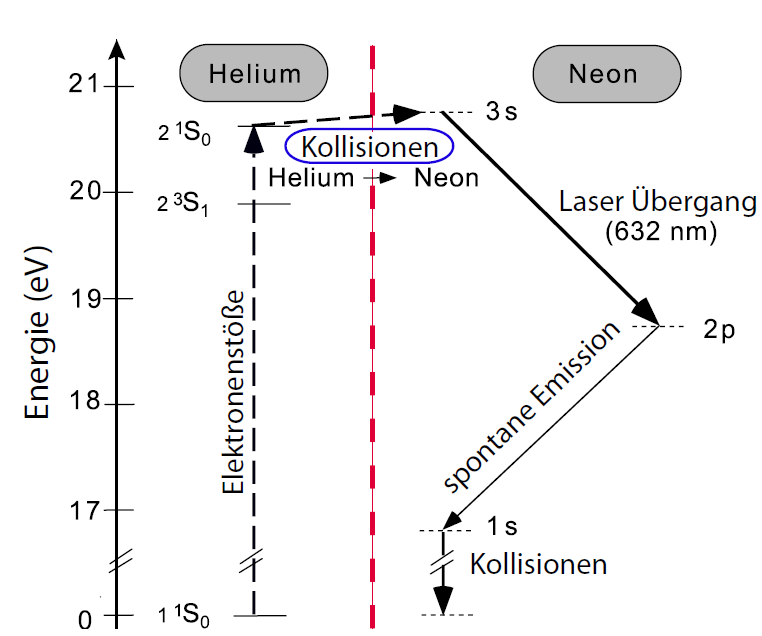
\includegraphics[width=0.75\linewidth]{Energielevel for He-Ne.png}
\caption{Energieleveldiagramm der Helium- und Neonatome. Der Energietransferprozess zur Erzeugung der Laserstrahlung ist schematisch dargestellt. \cite{praktikum}}
\label{fig:He-Ne}
\end{figure}
\FloatBarrier

Die notwendige Pumpenergie wird über eine elektrische Gasentladung bereitgestellt, welche Heliumatome in einen metastabilen angeregten Zustand versetzt. 
Die Energieniveaus dieser Zustände sind nahezu resonant mit dem 3s$_2$-Zustand der Neonatome (vgl. Abb. \ref{fig:He-Ne}). 
Durch inelastische Stoßprozesse kann so eine Energieübertragung erfolgen.

Befinden sich die Neonatome im 3s$_2$-Zustand, können sie durch stimulierte Emission in den 2p$_4$-Zustand übergehen. 
Dabei wird Licht mit einer charakteristischen Wellenlänge von 632,8 nm emittiert. 
Danach erfolgt eine spontane Emission zurück in den Grundzustand, wodurch der Prozess zyklisch abläuft.

Es existieren auch weitere Übergänge (z.B. im infraroten Bereich, siehe Abb.\ref{fig:Übergang}), die jedoch durch die Verwendung schmalbandiger Spiegel unterdrückt werden, da diese bevorzugt Licht im roten Spektralbereich reflektieren.

\FloatBarrier
\begin{figure}[htbp]
\centering
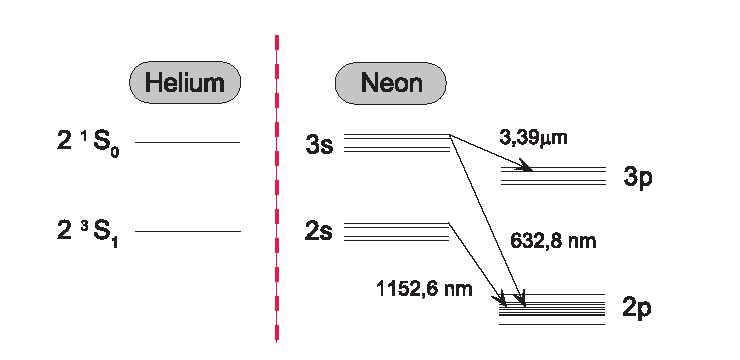
\includegraphics[width=0.75\linewidth]{mehrere Übergänge.png}
\caption{Weitere mögliche Übergänge im Neon-Atom. \cite{praktikum}}
\label{fig:Übergang}
\end{figure}
\FloatBarrier




\section{Aufbau}


Der komplette Aufbau erfolgt auf einer optischen Bank und erfordert besondere Sorgfalt und Justiergenauigkeit.

Zunächst wird die optische Achse definiert. 
Dazu kommt ein zusätzlicher, externer Laser (Pilotlaser) zum Einsatz, um die Achse möglichst präzise zu justieren.

\begin{figure}[htbp]
    \centering
    \begin{minipage}[t]{0.48\textwidth}
        \centering
        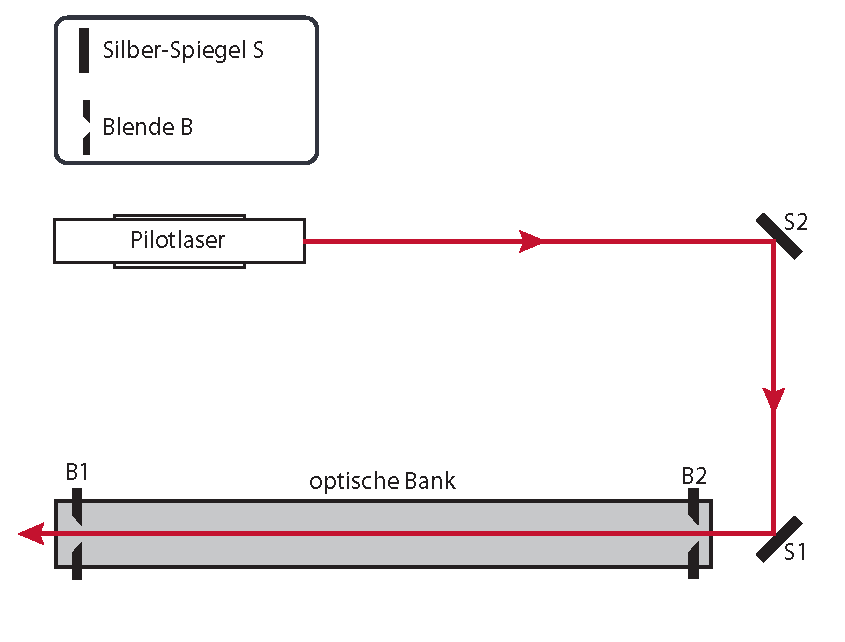
\includegraphics[width=\textwidth]{optische Achse.png}
       \caption{Justierung der optischen Achse mit Hilfe der Blenden. \cite{praktikum}}
        \label{fig:Blende}
    \end{minipage}
    \hfill
    \begin{minipage}[t]{0.48\textwidth}
        \centering
        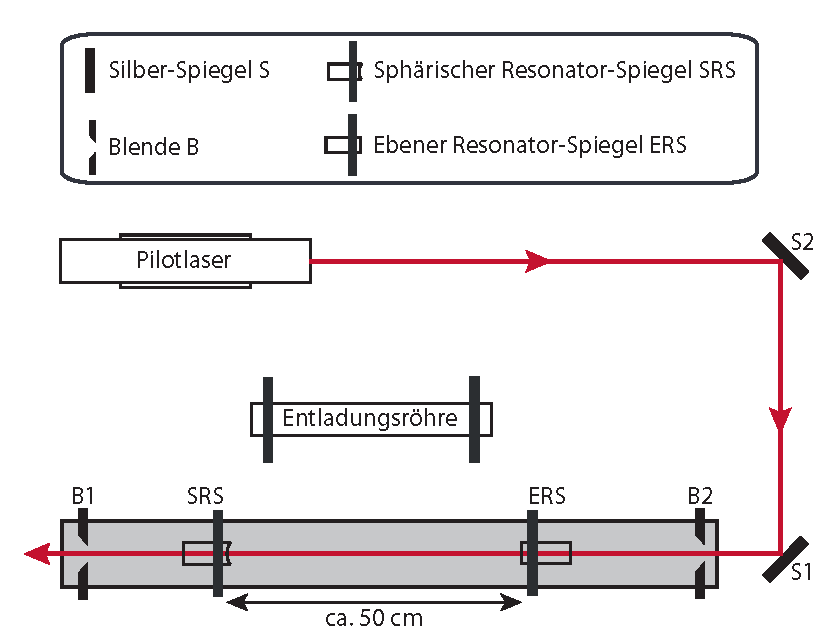
\includegraphics[width=\textwidth]{resonance spiegel.png}
        \caption{Justage der Resonatorspiegel. \cite{praktikum}}
        \label{fig:Spiegel}
   \end{minipage}
\end{figure}

Zuerst wird die Blende auf der optischen Achse ausgerichtet (Abb. \ref{fig:Blende}). 
Anschließend wird die Entladungsröhre eingebaut und so positioniert, dass möglichst wenig Licht innerhalb der Röhre verloren geht.
Danach erfolgt die Justage der Resonatorspiegel (einer sphärisch, einer planspiegelnd, halbdurchlässig), zunächst ohne Röhre. 
Ziel ist es, dass keine Reflexe mehr an der Wand sichtbar sind (vgl. Abb. \ref{fig:Spiegel}). 
Sobald dies erreicht ist, wird der Pilotlaser entfernt und die Entladungsröhre aktiviert. 
Durch feine Justierung der Spiegel sollte der Laser schließlich sichtbar aufblitzen – der Laser ist nun aktiv.



\chapter{Bestimmung der Wellenlänge}

Zur Wellenlängenbestimmung wird ein optisches Gitter außerhalb des Resonators hinter dem halbdurchlässigen Spiegel angebracht. 
Der Abstand der Interferenzmaxima kann dann über die Gleichungen

\begin{equation*}
    \tan(\alpha_i) = \frac{d_i}{a}
\end{equation*}
\begin{equation*}
    \sin(\alpha_i) = \frac{\delta}{g}; \qquad \text{mit} \qquad \delta = i \cdot \lambda
\end{equation*}
\begin{equation*}
    \Rightarrow \lambda = \frac{\sin\big(\arctan\big(\frac{d_i}{a}\big)\big)}{i \cdot g} \label{eq:Wellenlänge}
\end{equation*}
\begin{equation*}
    \Delta \lambda = \frac{1}{i \cdot g} \cdot \frac{1}{(d_i^2 + a^2)^\frac{3}{2}} \cdot \sqrt{(a^2 \cdot \Delta d)^2 + (da \cdot \Delta a
    )^2}
\end{equation*}

berechnet werden.
Mit der Gitterkonstanten $g = 600$ lines/mm und den gemessenen Werten ergibt sich folgende Tabelle:

\begin{table}[htbp]
    \centering
    \begin{tabular}{c|c|c|c}
        Ordnung & \(d_i ~[\text{m}]\) & \(a ~[\text{m}]\) & \(\lambda~[\text{nm}]\)\\
        \hline 
        -1 & 0,823 \(\pm\) 0,006 & 1,964 \(\pm\) 0,006 & 644,14 \(\pm\) 4,70 \\
        1 & 0,824 \(\pm\) 0,006 & 1,964 \(\pm\) 0,006 & 644,80 \(\pm\) 4,70 \\
    \end{tabular}
    \caption{Ermittelte Wellenlängen aus der ersten und negativen Ordnung.}
    \label{tab:Wellenlänge}
\end{table}


Der Mittelwert ergibt sich zu \(\lambda = (644,47 \pm 3,32)\)nm, was rund 1,8\% vom Literaturwert von 632,8 nm abweicht. 
Diese Differenz liegt außerhalb des angegebenen Fehlerbereichs und könnte auf eine fehlerhafte Gitterkonstante, nicht orthogonale Ausrichtung des Gitters oder auf eine systematische Fehlablesung zurückzuführen sein.


\chapter{Untersuchung der Polarisation}

Da das Laserlicht durch spontane Emission in alle Polarisationsrichtungen emittiert wird, wurde versucht, durch den Einsatz von Brewster-Fenstern eine Linearpolarisation zu erzwingen. 
Dabei nutzt man den Brewster-Winkel, bei dem Licht mit einer bestimmten Polarisationsrichtung bevorzugt transmittiert wird, während der orthogonal polarisierte Anteil reflektiert wird. 
Durch die Aneinanderreihung mehrerer Brewster-Fenster soll somit ein möglichst hoher Anteil linear polarisierten Lichts erzeugt werden.


Zur Untersuchung des Polarisationszustands wurde ein Polarisator in den Strahlengang eingebaut und die Intensität des transmittierten Lichts mit einer langsamen Photodiode gemessen (siehe Abb.~\ref{fig:Polar}).


\begin{figure}[H]
    \centering
    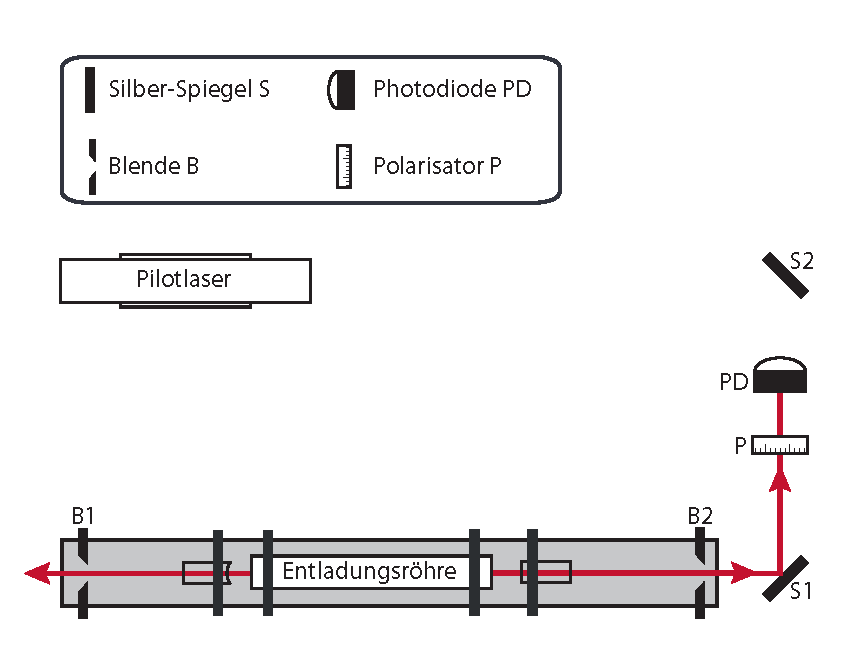
\includegraphics[width=0.75\linewidth]{Polarisation.png}
    \caption{Versuchsaufbau zur Untersuchung der Polarisation des Laserlichts. \cite{praktikum}}
   \label{fig:Polar}
\end{figure}

Die Spannung, die proportional zur Intensität ist, wurde in Abhängigkeit vom Polarisationswinkel gemessen. 
Ein vorgeschalteter $50~\Omega$-Widerstand wurde verwendet, um den Stromfluss zu vergrößern und die Messung zu erleichtern. 
Die gemessenen Werte sind in Tabelle~\ref{tab:Wellenlaenge} dargestellt.

\begin{table}[htbp]
    \centering
    \begin{tabular}{c|c}
        Winkel \(~[\text{°}]\) & Spannung \(U~[\text{mV}]\) \\
        \hline
        0 \(\pm\) 1 & 10 \(\pm\) 1{,}5 \\
        20 \(\pm\) 1 & 1{,}75 \(\pm\) 0{,}3 \\
        40 \(\pm\) 1 & 2 \(\pm\) 0{,}5 \\
        60 \(\pm\) 1 & 2{,}2 \(\pm\) 0{,}5 \\
        80 \(\pm\) 1 & 11{,}5 \(\pm\) 1 \\
        100 \(\pm\) 1 & 21 \(\pm\) 2 \\
        120 \(\pm\) 1 & 27{,}5 \(\pm\) 3 \\
        140 \(\pm\) 1 & 25 \(\pm\) 3 \\
        160 \(\pm\) 1 & 17 \(\pm\) 2 \\
        180 \(\pm\) 1 & 7{,}5 \(\pm\) 1 \\
        200 \(\pm\) 1 & 0{,}9 \(\pm\) 0{,}3 \\
        220 \(\pm\) 1 & 1{,}7 \(\pm\) 0{,}3 \\
        240 \(\pm\) 1 & 2{,}8 \(\pm\) 0{,}35 \\
        260 \(\pm\) 1 & 11 \(\pm\) 1 \\
        280 \(\pm\) 1 & 18 \(\pm\) 1{,}5 \\
        300 \(\pm\) 1 & 24 \(\pm\) 2 \\
        320 \(\pm\) 1 & 21 \(\pm\) 2 \\
        340 \(\pm\) 1 & 13 \(\pm\) 1{,}5 \\
    \end{tabular}
    \caption{Gemessene Spannungen bei unterschiedlichen Polarisationswinkeln}
    \label{tab:Wellenlaenge}
\end{table}

Da der Laser annähernd linear polarisiert ist, kann der Verlauf der Intensität in Abhängigkeit vom Polarisationswinkel durch das \textbf{Malus’sche Gesetz} beschrieben werden:

\begin{equation*}
    I = I_0 \cdot \cos^2(\theta - \theta_0) + b
\end{equation*}

Hierbei ist $I_0$ die maximale Intensität, $\theta_0$ der Winkel der Polarisationsebene und $b$ ein Offset (z.\,B. durch Umgebungslicht oder systematische Messfehler).

\begin{table}[htbp]
    \centering
    \begin{tabular}{c|c}
        Parameter & Wert \\
        \hline
        $U_0$ & (21{,}59 \(\pm\) 0{,}79) mV \\
        $\theta_0$ & (125{,}97 \(\pm\) 0{,}64) ° \\
        $b$ & (0{,}22 \(\pm\) 0{,}17) mV \\
    \end{tabular}
    \caption{Angepasste Parameter zur Beschreibung der Polarisation}
    \label{tab:WertePol}
\end{table}

Die zugehörige Ausgleichskurve ist in Abbildung~\ref{fig:PolarisationFigur} dargestellt.

\begin{figure}[H]
    \centering
    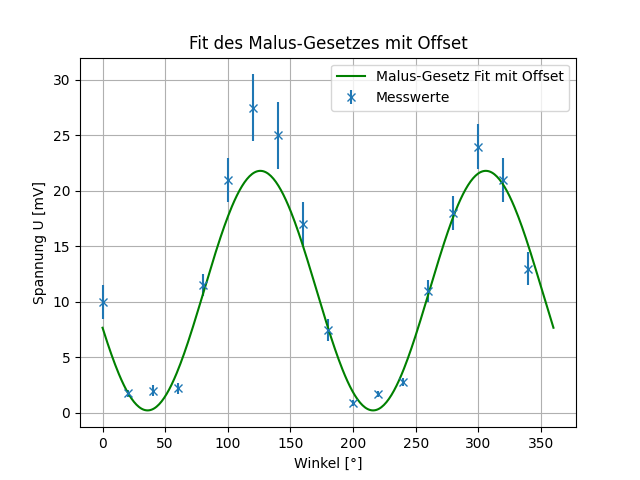
\includegraphics[width=0.75\linewidth]{Figure_2}
    \caption{Fit des Malus'schen Gesetzes an die Messwerte ($\chi^2_\text{red} = 5{,}16$)}
    \label{fig:PolarisationFigur}
\end{figure}

Es ist erkennbar, dass die Messwerte nicht vollständig mit dem Fit übereinstimmen.
Die reduzierte Chi-Quadrat-Abweichung $\chi^2_\text{red} = 5{,}16$ zeigt, dass der Fit nicht ideal ist, jedoch noch im akzeptablen Bereich liegt. 
Zusätzlich wurde eine Intensität ohne Polarisator von $I_0 = (33 \pm 1{,}5)~\text{mV}$ gemessen.

Die Abweichungen lassen sich durch verschiedene systematische Fehler erklären:

\begin{itemize}
    \item Der Polarisator war möglicherweise nicht korrekt ausgerichtet oder hatte interne Spannungen, die zu Doppelbrechung führen.
    \item Rückreflexionen oder Streulicht könnten das Messergebnis verfälscht haben.
    \item Die Intensitätsmessung war möglicherweise nicht vollständig stabil, sodass es zu Schwankungen kam.
\end{itemize}

Trotz der genannten Unstimmigkeiten lässt sich erkennen, dass die gemessenen Spannungen in guter Näherung dem Verlauf eines $\cos^2$-Gesetzes folgen, was das Malus’sche Gesetz bestätigt.

Der Polarisationsgrad \( PG \) des Lasers lässt sich aus den Fit-Parametern wie folgt berechnen:
\begin{equation*}
    PG = \frac{U_\text{max} - U_\text{min}}{U_\text{max} + U_\text{min}} = \frac{U_0 - b}{U_0 + b} = 0{,}98 \pm 0{,}01
\end{equation*}

Da der Polarisationsgrad kleiner als 1 ist, lässt sich daraus schließen, dass das Laserlicht nicht vollständig linear polarisiert ist. 
Ein geringer zirkular oder elliptisch polarisierter Anteil ist vorhanden. 
Dies ist zu erwarten, da die Brewster-Fenster nicht ideal sind und eine perfekte Polarisierung unter realen Bedingungen nicht erreicht werden kann.

\chapter{Messung des Strahlprofils}

In diesem Versuchsteil soll das Strahlprofil innerhalb des Resonators untersucht werden. 
Hierzu wird eine verstellbare Spaltblende (Messschieber) senkrecht zur Strahlachse montiert, sodass sie entlang der Querachse des Strahls verschoben werden kann. 
Auf diese Weise lässt sich die kritische Breite des Laserstrahls \( d(z) \) in Abhängigkeit von der Position \( z \) entlang des Strahlengangs bestimmen.

Durch schrittweise Verkleinerung der Spaltbreite wird der Strahl zunehmend beschnitten, was zu Verlusten im Resonator führt. 
Sobald diese Verluste größer sind als die Verstärkung im Lasermedium, bricht die Laseremission ab. 
Die kritische Spaltbreite hängt daher direkt vom lokalen Strahldurchmesser ab.

Das Strahlprofil eines idealen transversalen Grundmodus (TEM\textsubscript{00}) eines Gauß-Strahls folgt der bekannten Form:

\begin{equation*}
    w(z) = w_0 \cdot \sqrt{1+\left(\frac{z}{z_R}\right)^2}
\end{equation*}
 
mit einem Minimum der Strahlweite \( w_0 \) an der Stelle \( z = 0 \), der sogenannten Strahltaille. Für einen halbsymmetrischen Resonator mit einem planen und einem sphärischen Spiegel ergibt sich die theoretische Taille \( w_0 \) aus:

\begin{equation*}
    w_0 = \sqrt{\frac{\lambda}{\pi} \cdot \sqrt{L \cdot (R - L)}}
\end{equation*}

wobei \( L \) die Resonatorlänge (Abstand der Spiegel) und \( R \) der Krümmungsradius des sphärischen Spiegels ist. Die zugehörige Rayleigh-Länge ergibt sich zu:

\begin{equation*}
    z_R = \frac{\pi w_0^2}{\lambda}.
\end{equation*}

Da sich die Strahltaille bei einem halbsymmetrischen Resonator nahe am planen Spiegel befindet, wird die Position \( z = 0 \) auf diesen Punkt bezogen.

Zur Auswertung der Messdaten wurde die Form des Gaußstrahlradius

\begin{equation*}
    w(z) = d_0 \cdot \sqrt{1+\left(\frac{z}{z_R}\right)^2}
\end{equation*}

durch nichtlineare Regression an die experimentellen Daten angepasst. 
Dabei ist zu beachten, dass die gemessene kritische Spaltbreite \( d(z) \) nicht dem theoretischen Strahldurchmesser \( 2w(z) \) entspricht, sondern nur proportional dazu ist. Dieser Zusammenhang wird durch eine Proportionalitätskonstante \( c \) beschrieben:

\begin{equation}
    2 \cdot w(z) = c \cdot d(z)
    \label{eq:proportionalitaet}
\end{equation}

Die folgenden Tabellen zeigen die gemessenen Werte der kritischen Spaltbreite \( d(z) \) in Abhängigkeit von der Position \( z \) für zwei unterschiedliche Resonatorlängen:

\begin{table}[htbp]
    \centering
    \begin{tabular}{S[table-format=1.2(2)]|S[table-format=3.0(1)]}
        {$d(z)\,\si{\milli\meter}$} & {$z\,\si{\milli\meter}$} \\
        \hline
        1.35 \pm 0.01 & 3 \pm 1 \\
        2.20 \pm 0.01 & 401 \pm 1 \\
        2.25 \pm 0.01 & 415 \pm 1 \\
        2.50 \pm 0.01 & 445 \pm 1 \\
        2.60 \pm 0.01 & 487 \pm 1 \\
        2.70 \pm 0.01 & 505 \pm 1 \\
    \end{tabular}
    \caption{Messung des Strahlprofils bei einer Resonatorlänge von \SI{62.0}{\centi\meter}}
    \label{tab:62}
\end{table}

\begin{table}[htbp]
    \centering
    \begin{tabular}{S[table-format=1.2(2)]|S[table-format=3.0(1)]}
        {$d(z)\,\si{\milli\meter}$} & {$z\,\si{\milli\meter}$} \\
        \hline
        1.90 \pm 0.01 & 12 \pm 1 \\
        3.80 \pm 0.01 & 506 \pm 1 \\
        4.90 \pm 0.01 & 555 \pm 1 \\
        5.85 \pm 0.01 & 635 \pm 1 \\
    \end{tabular}
    \caption{Messung des Strahlprofils bei einer Resonatorlänge von \SI{76.3}{\centi\meter}}
    \label{tab:76_3}
\end{table}

Die durch Ausgleichsrechnung bestimmten Parameter sowie die theoretischen Vergleichswerte sind in Tabelle~\ref{tab:BStrahl} zusammengefasst:

\begin{table}[htbp]
    \centering
    \begin{tabular}{S|S|S|S|S|S}
        {$L\,\si{\centi\meter}$} & {$d_0\,\si{\micro\meter}$} & {$z_R\,\si{\centi\meter}$} &
        {$w_{0,\text{theo}}\,\si{\micro\meter}$} & {$z_{R,\text{theo}}\,\si{\centi\meter}$} & {$c$} \\
        \hline
        62.0 \pm 0.3 & 1332 \pm 49 & 29.15 \pm 1.56 & 312 & 48.54 & 0.469 \pm 0.017 \\
        76.3 \pm 0.3 & 1831 \pm 50 & 24.67 \pm 0.82 & 292 & 42.52 & 0.319 \pm 0.009 \\
    \end{tabular}
    \caption{Experimentell bestimmte und theoretisch berechnete Strahlparameter}
    \label{tab:BStrahl}
\end{table}

Die zugehörigen Ausgleichskurven sind in den folgenden Abbildungen dargestellt:

\begin{figure}[htbp]
    \centering
    \begin{subfigure}[t]{0.48\textwidth}
        \centering
        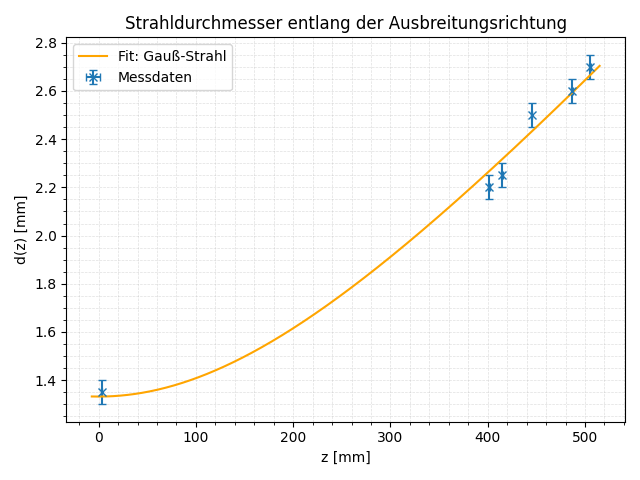
\includegraphics[width=\textwidth]{Figure_3.png}
        \caption{Strahlprofil für \(L = \SI{62.0}{\centi\meter}\), \(\chi^2 = 1{,}52\)}
        \label{fig:62}
    \end{subfigure}
    \hfill
    \begin{subfigure}[t]{0.48\textwidth}
        \centering
        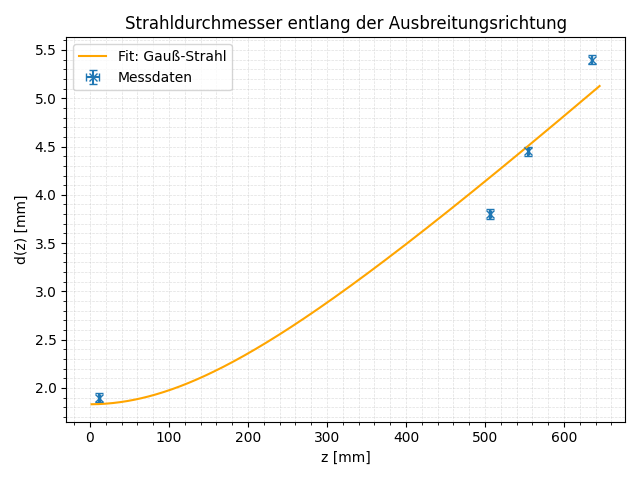
\includegraphics[width=\textwidth]{Figure_4.png}
        \caption{Strahlprofil für \(L = \SI{76.3}{\centi\meter}\), \(\chi^2 = 53{,}80\)}
        \label{fig:76}
    \end{subfigure}
    \caption{Gemessene Strahlprofile mit Fitkurven}
\end{figure}

Die Anpassung bei \(L = \SI{62.0}{\centi\meter}\) gelingt deutlich besser als bei \(L = \SI{76.3}{\centi\meter}\), was sich auch im stark erhöhten \(\chi^2\)-Wert für den zweiten Fall widerspiegelt. 
Ursachen hierfür könnten die geringere Anzahl an Messpunkten sowie experimentelle Schwierigkeiten beim Ansetzen der Spaltblende sein, insbesondere bei größeren Spaltweiten, bei denen der Laser noch nicht vollständig erlischt.

Ein Vergleich der experimentell bestimmten Rayleigh-Längen mit den theoretisch erwarteten Werten zeigt eine Abweichung von etwa 40\,\%. 
Diese Diskrepanz könnte durch systematische Fehler bei der Ablesung sowie durch eine fehlerhafte Ausrichtung der Spaltblende verursacht sein: 
Ist diese nicht exakt senkrecht zur Strahlachse positioniert, erscheint die effektive Spaltbreite kleiner, was zu einer Überschätzung des Strahldurchmessers führt.

Zudem ist zu beachten, dass die gemessene Spaltbreite nicht direkt dem \SI{1}{/e^2}-Durchmesser des Laserstrahls entspricht. 
Der Strahlradius \( w(z) \) beschreibt den Abstand von der Strahlachse, bei dem die Intensität auf \( 1/e^2 \) ihres Maximalwertes abgesunken ist. 
Die Abschattung durch die Blende führt jedoch bereits bei größerer Intensität zu einem Erlöschen der Emission.

Aus diesem Grund wurde eine Proportionalitätskonstante \( c \) eingeführt, um den Zusammenhang zwischen dem theoretischen Strahldurchmesser und der experimentell bestimmten kritischen Spaltbreite herzustellen. 
Diese Beziehung ist in Gleichung~\eqref{suchung_c} gegeben:

\begin{equation}
    2 \cdot w(z) = c \cdot d(z)
    \label{suchung_c}
\end{equation}

Der Mittelwert der ermittelten Proportionalitätskonstanten beträgt:

\begin{equation*}
    c = 0{,}394 \pm 0{,}008
\end{equation*}

Damit lässt sich die kritische Spaltbreite in einen effektiven Strahldurchmesser überführen. 
Diese Konstante stellt somit eine zentrale experimentelle Größe dar, die den Abgleich zwischen theoretischem Modell und praktischer Messung ermöglicht.
 \chapter{ Aufbau der optischen Diode}

Um eine destabilisierende Rückkopplung in den He-Ne-Resonator zu verhindern, setzen wir den Isolator ein, der im \cref{fig:function_of_optical_diode} dargestellt ist. 
Brewster-Fenster, so angebracht, dass sie im Brewster-Winkel \cite{introtoED} 
\begin{equation}
  \tan\theta_B = \bigl(\tfrac{n_{\mathrm{glas}}}{n_{\mathrm{luft}}}\bigr),
\end{equation}
stehen, dienen als erster Polarisationsfilter innerhalb der Kavität. 
Bei diesem Winkel passiert p-polarisiertes Licht (mit elektrischem Feld in der Einfallsebene) die Glas-Luft-Grenzfläche ohne Reflexion, während s-polarisiertes Licht (Feld senkrecht zur Einfallsebene) teilweise reflektiert und somit unterdrückt wird. 
Dadurch ist der intra-kavitär austretende Strahl am Ausgangskoppler bereits stark linear entlang der p-Achse polarisiert und liefert einen sauberen Eingangsstatus für die nachfolgenden Isolator-Komponenten.

\begin{figure}[htbp]
  \centering
  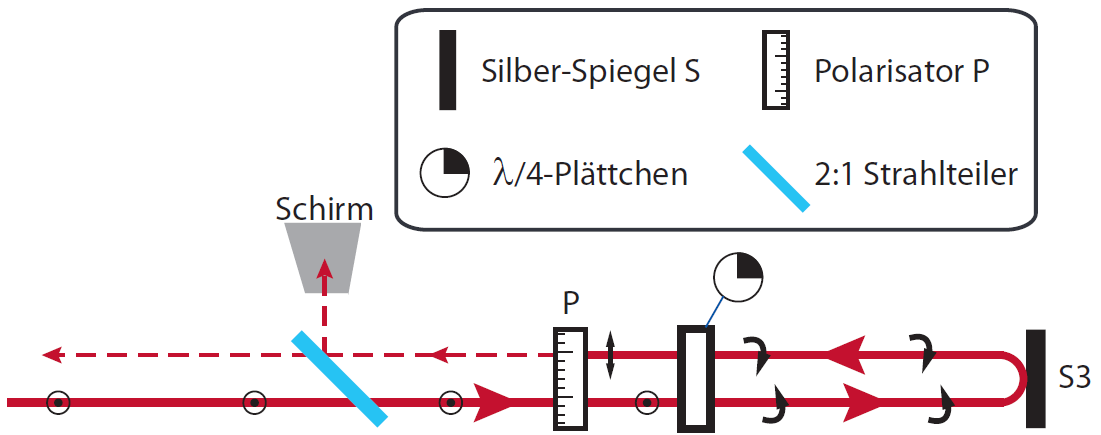
\includegraphics[width=0.75\linewidth]{Funktion der optischen Diode.png}
  \caption{Funktionsprinzip des optischen Isolators: Der rückwärts laufende Strahl ist zur Veranschaulichung leicht versetzt dargestellt. Schwarze Pfeile entlang des Strahlengangs zeigen mögliche Polarisationszustände in den einzelnen Stufen an. \cite{praktikum}}
  \label{fig:function_of_optical_diode}
\end{figure}

Der Isolator selbst besteht aus einem linearen Polarisator (P), einer Viertelwellenplatte ($\lambda/4$) und einem Silber-Spiegel (S3), die unmittelbar hinter dem Ausgangskoppler in Serie angeordnet sind (siehe \cref{fig:aufbau_mit_optischer_diode}). 
Auf dem Vorwärtsdurchgang überträgt P nur das p-polarisierte Licht, welches die $\lambda/4$-Platte in rechtszirkulare Polarisation umwandelt. 
Nach der Reflexion an S3 - die Drehrichtung beibehält - durchläuft der Rückstrahl erneut die $\lambda/4$-Platte und tritt als um 90° gedrehtes, nun s-polarisiertes Licht aus. 
Dieses gedrehte Licht wird von P blockiert, sodass eine hohe nicht-reziproke Isolation erreicht wird, ohne nennenswerte Einfügedämpfung im Vorwärtsweg.
\begin{figure}[htbp]
  \centering
  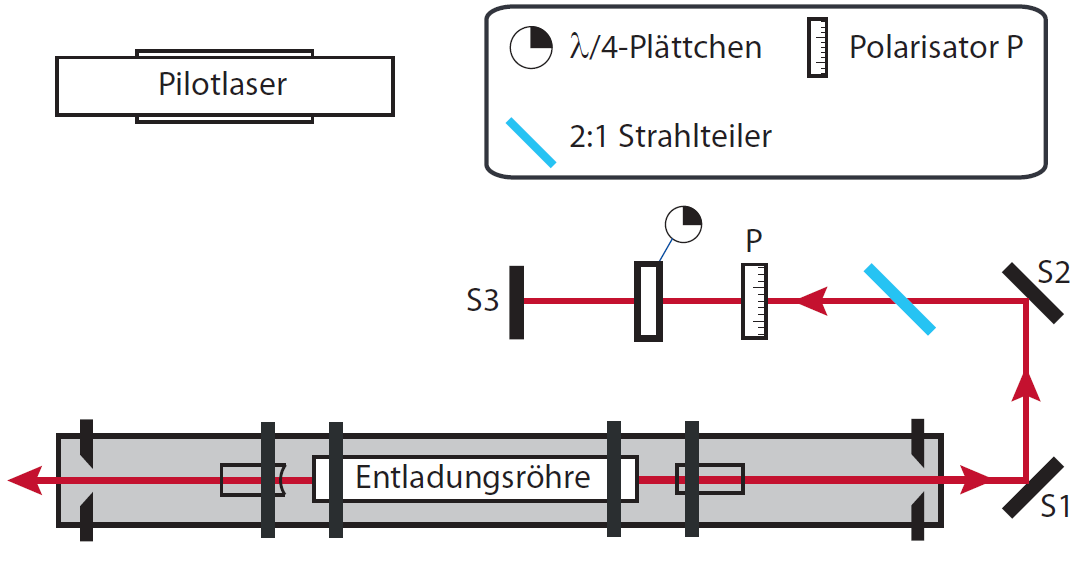
\includegraphics[width=0.75\linewidth]{Aufbau mit optischer Diode.png}
  \caption{Aufbau mit optischer Diode \cite{praktikum}}
  \label{fig:aufbau_mit_optischer_diode}
\end{figure}

Mechanisch sind der Polarisator, die $\lambda/4$-Platte und ein nicht-polarisierender Strahlteiler im Verhältnis 2 : 1 in Justierhaltern montiert, die feines Kippen und Drehen sowie axiale Ausrichtung erlauben. 
Der Strahlteiler führt etwa ein Drittel des Vorwärtslichts zu einer Leistungsüberwachung ab, während der Rest zur schnellen Photodiodenkette gelangt. Alle Optiken verfügen über breitbandige Antireflexbeschichtungen, um Streureflexionen zu minimieren.

\paragraph{Justage-Prozedur:}
\begin{enumerate}
  \item \textbf{Polarisator-Orientierung:} Drehen Sie P, bis die durch den Monitorport gemessene Leistung maximal ist, um die native p-Polarisation des Lasers einzustellen.
  \item \textbf{Viertelwellenplatten-Einstellung:} Entfernen Sie S3 und justieren Sie die $\lambda/4$-Platte, bis die schwache Rückreflexion durch P auf einem Schirm verschwindet - ein Zeichen für eine perfekte 90°-Drehung der rücklaufenden Polarisation.
  \item \textbf{Isolations-Überprüfung:} Setzen Sie S3 wieder ein und vergewissern Sie sich, dass kein messbarer Rückfluss durch P auftritt, während die Vorwärtsdurchlässigkeit unverändert bleibt.  
\end{enumerate}
Während der Justage wurde der Polarisator auf $\theta = 290^\circ \pm 1^\circ$ und die Viertelwellenplatte auf $\lambda/4 = 64^\circ \pm 1^\circ$ eingestellt.


%===============================================================================================================================================================================================================================================================================================================================================
\chapter{Optischer Spektrumanalysator} \label{sec:5.7}

Nach Verlassen des Isolators wird der He-Ne-Strahl in einen konfokalen Fabry-Perot-Resonator (\cref{fig:Spektrumanalysator}) mit äußerer Länge $l_{\mathrm{ext}} = 5{,}0\,\si{\centi\meter}$ eingekoppelt. \\
Nach Handbuch \cite{praktikum} sind dessen Eigenfrequenzen
\begin{equation}
  \nu_{qnm}
  = \Bigl(q + \tfrac{m+n+1}{2}\Bigr)\,\frac{c}{2\,l}.
\end{equation}
Gleiche transversale Moden TEM$_{nm}$ liegen damit im Abstand des freien Spektralbereichs
\begin{equation*}
  \Delta\nu_{\mathrm{FSR}}
  = \frac{c}{2\,l},
\end{equation*}
während benachbarte Moden um
\begin{equation*}
  \Delta\nu
  = \frac{c}{4\,l}
\end{equation*}
getrennt sind.
\begin{figure}[htbp]
  \centering
  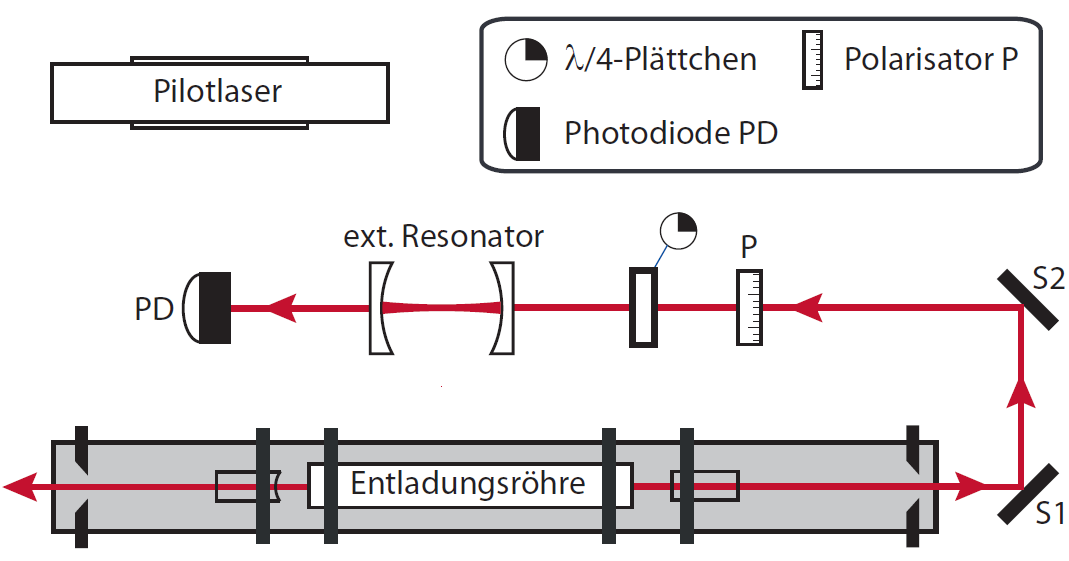
\includegraphics[width=0.75\linewidth]{Aufbaus zum optischen Spektrumanalysator.png}
  \caption{Schema des Aufbaus zum optischen Spektrumanalysator \cite{praktikum}}
  \label{fig:Spektrumanalysator}
\end{figure}

Ein Piezoaktor verändert $l_{\mathrm{ext}} = 5 \si{\cm}$ um etwa $200\,\si{\nm}$ bei einer $0-100 \si{\volt}  $/$50 \si{\hertz}$-Dreiecksspannung, so dass ein vollständiger Sweep genau eine $\Delta\nu_{\mathrm{FSR}}$ abtastet. 
Kanal 1 des Oszilloskops zeigt die Piezo-Spannung $U(t)$, Kanal 2 die transmittierte Intensität $I(t)$ einer langsamen Photodiode, was eine Folge von Übertragungsclustern wie zwischen \cref{fig:9a} bis \cref{fig:9c} ergibt. 
Die korrekte Justage erfolgte mittels Papierziel- und Zwei-Spiegel-Kippverfahren (\cref{fig:Resonator}), bis für jede Piezo-Position ein einziger scharfer Spot auftrat und die Peaks minimal verbreitert waren.
\begin{figure}[htbp]
  \centering
  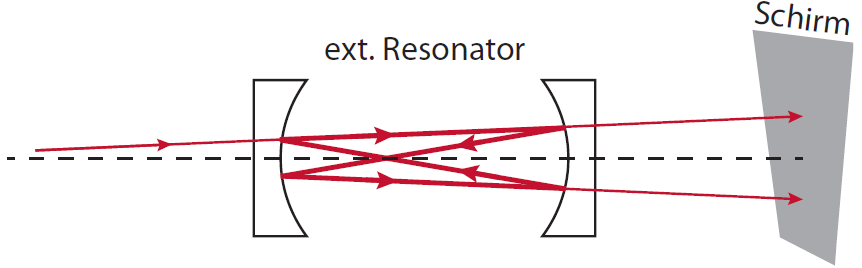
\includegraphics[width=0.75\linewidth]{Resonator bei Dejustage.png}
  \caption{Strahlengang im externen Resonator bei Dejustage \cite{praktikum}}
  \label{fig:Resonator}
\end{figure}
\begin{figure}[htbp]
    \centering
    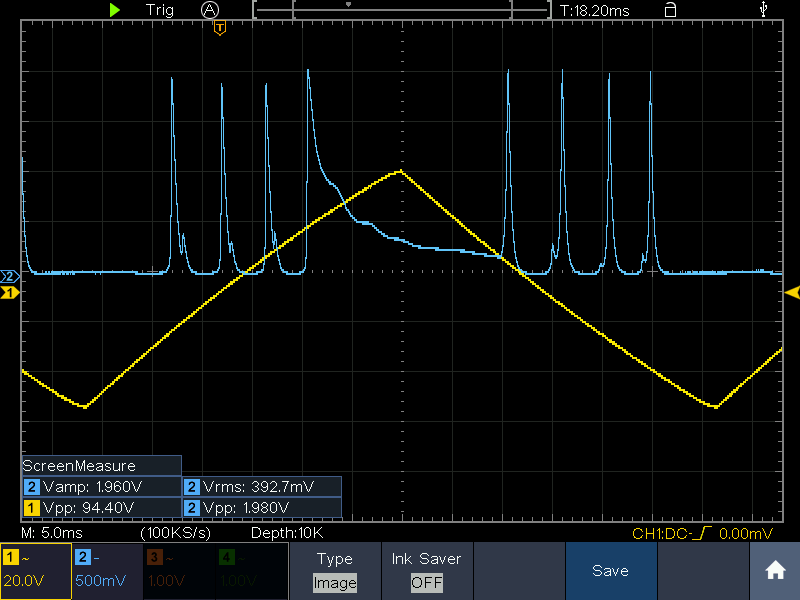
\includegraphics[width=0.75\linewidth]{52_1a.png}
     \caption{Oszilloskopübertragungscluster interne Kavitätenlängen $l = 52,0\,\si{\centi\meter} \pm$ 0{,}4\,\si{\centi\meter}.}
    \label{fig:9a}
\end{figure}
  \begin{figure}[htbp]
    \centering
    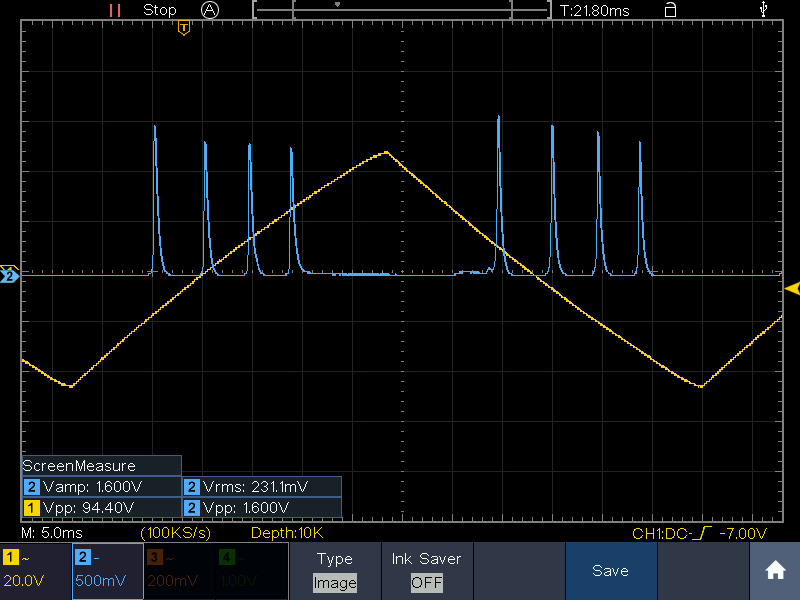
\includegraphics[width=0.75\linewidth]{68_1a.png}
     \caption{Oszilloskopübertragungscluste interne Kavitätenlängen $l = 68,0\,\si{\centi\meter} \pm$ 0{,}3\,\si{\centi\meter}.}
    \label{fig:9b}
  \end{figure}
  \newpage
  \begin{figure}[htbp]
    \centering
    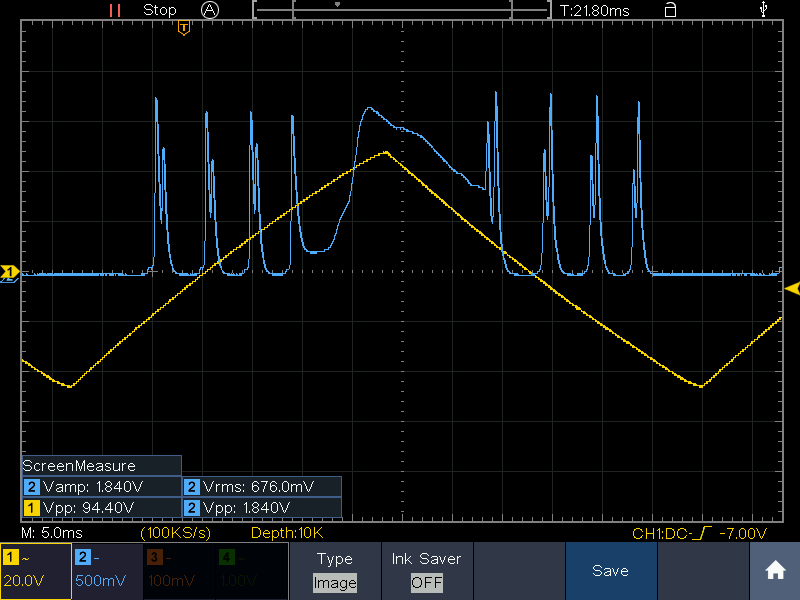
\includegraphics[width=0.75\linewidth]{80_1a.png}
     \caption{Oszilloskopübertragungscluster interne Kavitätenlängen $l = 80,0\,\si{\centi\meter} \pm$ 0{,}3\,\si{\centi\meter}.}
    \label{fig:9c}
  \end{figure}
 
 Für jede Oszilloskop-Spur bestimmen wir zwei Zeitintervalle: $a$, die horizontale Ausdehnung eines gesamten Übertragungsclusters (entspricht einer freien Spektralbreite des externen Fabry-Perot-Analysators), und $b$, der Abstand zweier benachbarter Peaks innerhalb dieses Clusters (entspricht dem longitudinalen Modenabstand der internen He-Ne-Kavität). 
 Da sowohl $a$ als auch $b$ auf derselben (möglicherweise nichtlinearen) Piezo-Zeitachse abgelesen werden, kompensiert ihr Verhältnis jede unbekannte Kalibrierkonstante. Damit lassen sich drei Frequenzintervalle definieren.

Die freie Spektralbreite des Analysators ist
\begin{equation}
  \Delta\nu_{\mathrm{FSR}}
  = \frac{c}{2\,l_{\mathrm{ext}}}
  = \frac{299\,792\,458\;\mathrm{m/s}}{2 \times 0{,}050\;\mathrm{m}}
  \approx 3{,}00\;\mathrm{GHz},
\end{equation}
wobei $l_{\mathrm{ext}} = 5{,}0\;\mathrm{cm}$.

Der experimentell bestimmte Modenabstand des Lasers ergibt sich zu
\begin{equation}
 \Delta\nu_{\mathrm{exp}}
  = \frac{b}{a}\;\Delta\nu_{\mathrm{FSR}},
\end{equation}
mit der Fehlerfortpflanzung
\begin{equation}
  \delta\Delta\nu_{\mathrm{exp}}
  =\Delta\nu_{\mathrm{exp}}
    \sqrt{\Bigl(\frac{\delta b}{b}\Bigr)^{2}
        + \Bigl(\frac{\delta a}{a}\Bigr)^{2}
        + \Bigl(\frac{\delta l}{l}\Bigr)^{2}}\!,
\end{equation}
wobei die Cursor-Unsicherheiten $\delta a = 0{,}20\;\mathrm{ms}$ und $\delta b = 0{,}20\;\mathrm{ms}$ sowie die Längenunsicherheiten $\delta l_{52} = 0{,}4\;\mathrm{cm}$ und $\delta l_{68} = \delta l_{80} = 0{,}3\;\mathrm{cm}$ betragen.

Der theoretische Modenabstand für eine ideale planparallele Kavität der Länge $l$ ist
\begin{equation}
 \Delta\nu_{\mathrm{theo}}
  = \frac{c}{2\,l},
  \quad
  \delta\Delta\nu_{\mathrm{theo}}
  =\Delta\nu_{\mathrm{theo}}\,\frac{\delta l}{l}.
\end{equation}

\begin{table}[H]
  \centering
  \resizebox{0.8\columnwidth}{!}{%
    \begin{tabular}{|c|c|c|c|c|}
      \hline
      $l \,\;\pm\delta l \,/\mathrm{cm}$ 
        & $a \,\pm \delta a\,/\mathrm{ms}$ 
        & $b \,\pm \delta b\,/\mathrm{ms}$ 
        & $v_{\mathrm{exp}}\pm\delta\Delta\nu_{\mathrm{exp}}\;/\;\mathrm{MHz}$ 
        & $v_{\mathrm{theo}}\pm\delta\Delta\nu_{\mathrm{theo}}\;/\;\mathrm{MHz}$ \\ \hline
      $52{,}0 \pm 0{,}4$   & $25{,}0 \pm 0{,}2$ & $3{,}0 \pm 0{,}2$ & $360 \pm 13$ & $288 \pm 2$ \\ \hline
      $68{,}0 \pm 0{,}3$   & $25{,}0 \pm 0{,}2$ & $2{,}0 \pm 0{,}2$ & $240 \pm 12$ & $220 \pm 1$ \\ \hline
      $80{,}0 \pm 0{,}3$   & $25{,}0\pm 0{,}2$ & $1{,}5 \pm 0{,}2$ & $180 \pm 12$ & $187 \pm 1$ \\ \hline
    \end{tabular}%
  }
  \caption{Experimentelle und theoretische Modenabstände für drei interne Kavitätenlängen.}
  \label{tab:mode-spacings}
\end{table}

Der Modenabstand nimmt proportional zu $1/l$ ab, wie genau vorhergesagt. 
Für $l = 68\,\mathrm{cm}$ und $l = 80\,\mathrm{cm}$ liegen die experimentellen Werte innerhalb ihrer kombinierten Unsicherheiten mit den theoretischen Vorhersagen überein, was sowohl die Kalibrierung des Analysators als auch die Gültigkeit der einfachen Formel$ \frac{c}{2\,l}$ für den Laser bestätigt. 
Die Messung bei $l = 52\,\mathrm{cm}$ weicht um etwa 25\,\% ab, höchstwahrscheinlich, weil der Cursor für $b$ zwischen nicht-benachbarten Peaks gesetzt oder die Clustergrenze für $a$ falsch identifiziert wurde; eine Wiederholung dieser Aufnahme mit verfeinerter Cursor-Positionierung sollte sie in Übereinstimmung mit den anderen beiden Ergebnissen bringen.

Die Unsicherheiten werden hauptsächlich durch die Cursor-Platzierung und die mit dem Maßband bestimmte Längenunsicherheit $\delta l$ dominiert. Systematische Fehler wie Piezo-Hysterese oder Nichtlinearität der Sweep-Geschwindigkeit heben sich im Verhältnis $b/a$ auf, während verbleibende Spiegel-Dejustagen durch iteratives Feinkippen unterdrückt wurden, bis keine weitere Verengung der Peak-Breiten möglich war. Zukünftige Verbesserungen sind straightforward: Das Speichern der Rohspuren als CSV-Dateien ermöglicht Lorentz-Fits, die $\delta a$ und $\delta b$ auf unter $0{,}02\,\mathrm{ms}$ reduzieren würden, und der Ersatz des Maßbands durch einen Messschieber ($\pm .05 \si{/cm}$) würde $\delta l / l$ in den $10^{-3}$-Bereich senken. Mit diesen Optimierungen sollten alle drei Kavitätenlängen das Gesetz $1/l$ auf besser als 1\,\% bestätigen und eine noch genauere Überprüfung der Analysator-Kalibrierung liefern.



%===============================================================================================================================================================================================================================================================================================================================================
\chapter{ Präzise Messung des Modenabstandes mittels einer
optischen Schwebung} \label{sec:5.8}

Nach der optischen Bestimmung des Modenabstands in \cref{sec:5.7} wird dieselbe Größe nun auf einer absoluten RF-Skala gemessen, indem zwei longitudinale Moden auf einer schnellen Photodiode überlagert und das Misch-IF-Signal auf einem 350 MHz-Oszilloskop analysiert wird \cref{fig:difffreq}. Zwei benachbarte Kavitätsfrequenzen $\nu_{1} = \omega_{1}/2\pi$ und $\nu_{2} = \omega_{2}/2\pi$ erzeugen nach quadratischer Detektion einen RF-Term bei der Differenzfrequenz
\begin{equation*}
  \Delta\omega = \omega_{1} - \omega_{2} = 2\pi\,\Delta\nu_{\mathrm{beat}},
\end{equation*}
wobei alle hochfrequenten Summen- und $2\omega$-Terme oberhalb der 35 MHz-Low-Pass-Grenze des Mixers liegen und somit unterdrückt werden. Die ganze Zahl $m$ bezeichnet die Anzahl der longitudinalen Intervalle zwischen den beiden Moden ($m=1$ für benachbarte Moden, $m=2$ für jeden zweiten Modenabstand usw.), sodass gilt
\begin{equation}
  \Delta\nu_{\mathrm{beat}} = m\,\Delta\nu_{\mathrm{laser}}.
\end{equation}

\begin{figure}[htbp]
    \centering
    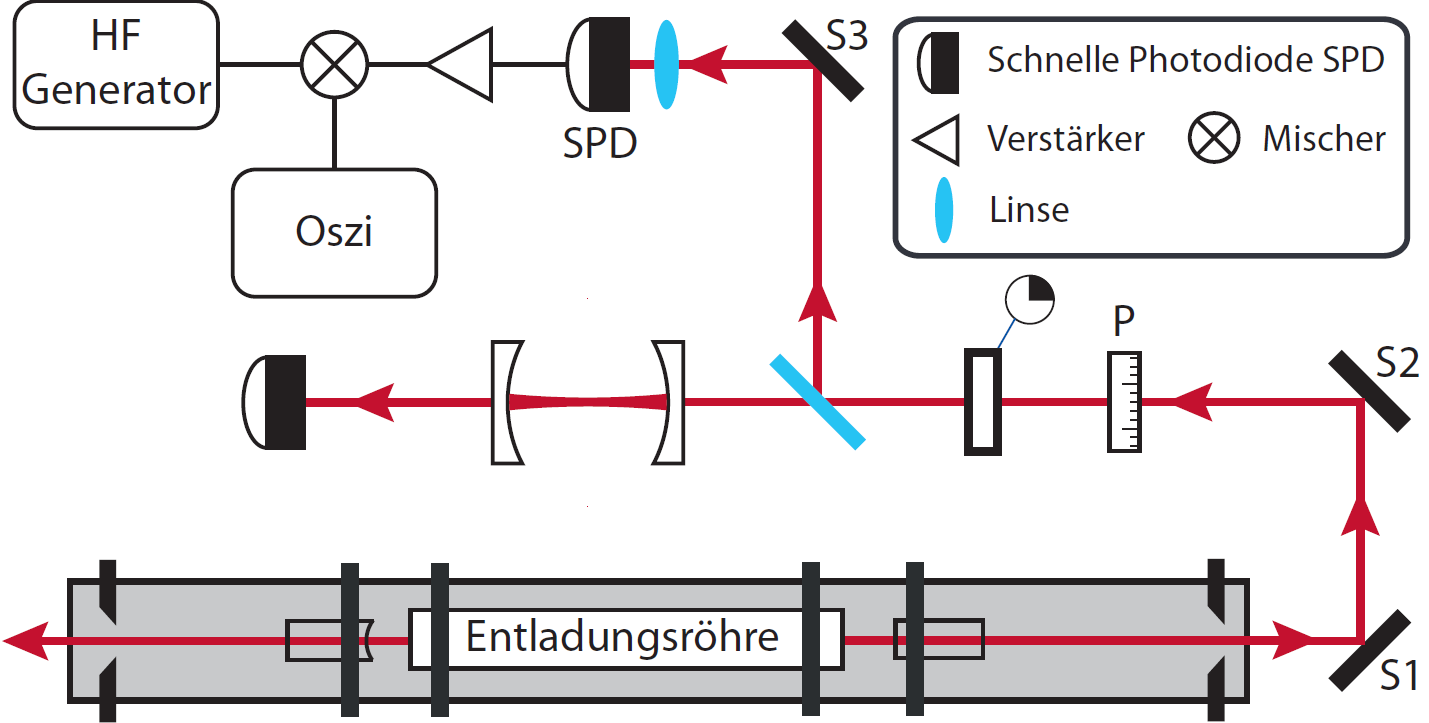
\includegraphics[width=0.75\linewidth]{Differenzfrequenz verschiedener.png}
     \caption{Schematischer Aufbau zur präzisen Messung der Differenzfrequenz verschiedener longitudinaler Moden \cite{praktikum}}
    \label{fig:difffreq}
  \end{figure}

Der IF-Ton $f$ wurde mit Oszilloskop-Cursorn abgelesen; seine Halbwertsbreite (HWHM) liefert die statistische Unsicherheit $\delta f$. Für unsere Spuren beträgt HWHM etwa $0{,}10\,\mathrm{MHz}$ für $m=1$ und $0{,}50\,\mathrm{MHz}$ für $m=2$. Der experimentelle Modenabstand ergibt sich zu
\begin{equation}
  \Delta\nu_{\mathrm{exp}} = \frac{f}{m}, 
  \qquad
  \delta(\Delta\nu_{\mathrm{exp}}) = \frac{\delta f}{m}.
\end{equation}

Der theoretische Modenabstand einer idealen planparallelen Kavität der Länge $l$ lautet
\begin{equation}
  \Delta\nu_{\mathrm{theo}} = \frac{c}{2\,l}, 
  \qquad
  \delta(\Delta\nu_{\mathrm{theo}}) = \Delta\nu_{\mathrm{theo}}\,\frac{\delta l}{l},
\end{equation}
mit $c = 299\,792\,458\;\mathrm{m/s}$. Die Längen wurden mit einem Stahlmaßband gemessen; $\delta l_{52} = 0{,}4\,\mathrm{cm}$ und $\delta l_{68,70.8,80} = 0{,}3\,\mathrm{cm}$.

\begin{table}[H]
  \centering
  \resizebox{0.8\columnwidth}{!}{%
    \begin{tabular}{|c|c|c|c|c|}
      \hline
      $l \pm \delta l \;/\si{\centi\meter}$ & $m$ & $f\; \pm \delta f\;/\si{\mega\hertz}$ &
      $\Delta\nu_{\mathrm{exp}}\pm\delta(\Delta\nu_{\mathrm{exp}})\;/\si{\mega\hertz}$ &
      $\Delta\nu_{\mathrm{theo}}\pm\delta(\Delta\nu_{\mathrm{theo}})\;/\si{\mega\hertz}$ \\ \hline
      $52{,}0\pm0{,}4$ & 1 & $303{,}7  \pm 0{,}10$ & $303{,}7\pm0{,}10$ & $288{,}3\pm2{,}2$ \\ \hline
      $68{,}0\pm0{,}3$ & 1 & $135{,}7  \pm  0{,}10 $ & $135{,}7\pm0{,}10$ & $220{,}4\pm1{,}0$ \\ \hline
      $68{,}0\pm0{,}3$ & 2 & $309{,}9  \pm  0{,}50 $ & $154{,}9\pm0{,}25$ & $220{,}4\pm1{,}0$ \\ \hline
      $70{,}8\pm0{,}3$ & 1 & $219{,}2  \pm 0{,}10 $ & $219{,}2\pm0{,}10$ & $211{,}7\pm0{,}9$ \\ \hline
      $70{,}8\pm0{,}3$ & 2 & $441{,}8  \pm  0{,}50 $ & $220{,}9\pm0{,}25$ & $211{,}7\pm0{,}9$ \\ \hline
      $80{,}0\pm0{,}3$ & 1 & $175{,}7  \pm  0{,}10 $ & $175{,}7\pm0{,}10$ & $187{,}4\pm0{,}7$ \\ \hline
      $80{,}0\pm0{,}3$ & 2 & $347{,}5  \pm  0{,}50$ & $173{,}8\pm0{,}25$ & $187{,}4\pm0{,}7$ \\ \hline
    \end{tabular}%
  }
  \caption{Beats von $m=1$ und $m=2$ Moden: experimentelle und theoretische Modenabstände für verschiedene interne Kavitätenlängen.}
  \label{tab:beat-data}
\end{table}

Die Messungen für $m=1$ und $m=2$ bei $l=70{,}8\,\mathrm{cm}$ stimmen untereinander und mit $\Delta\nu_{\mathrm{theo}}$ auf besser als 4\,\% überein, was bestätigt, dass die 441{,}8 MHz-Linie tatsächlich das zweite Harmonische des Modenabstands darstellt. Bei $l=80{,}0\,\mathrm{cm}$ umschließen die beiden Harmonischen den theoretischen Wert von 187 MHz innerhalb von 7\,\%.  
Die Ausreißer bei $l = 52\,\si{\centi\meter}$ und $l = 68\,\si{\centi\meter}$ lassen sich auf \emph{Modenkontamination} zurückführen: Nach diesen Messreihen zeigte der konfokale Analysator eine schwache dritte longitudinale Mode etwa 6 dB unter den Hauptlinien, sodass die Photodiode tatsächlich mehrere Beat-Frequenzen statt nur $\omega_{1} - \omega_{2}$ detektierte. Bei 52 cm verschieben die überlagerten RF-Töne den intensitätsgewichteten Schwerpunkt nach oben und treiben $\Delta\nu_{\mathrm{exp}}$ auf 303,7 MHz anstatt der aus $c/(2l)$ zu erwartenden 288 MHz. Bei 68 cm wurde beim ersten Durchlauf ein $m=2$-Beat (Zwei-Intervall-Abstand) fälschlich als $m=1$ interpretiert, was den künstlich niedrigen Wert von 135,7 MHz ergab. Auch die zweite Aufnahme, obwohl korrekt mit $m=2$ beschriftet, litt unter ungleichen Modenamplituden und landete zwischen Grundfrequenz und erstem Harmonischen. Kurz gesagt: Eine zusätzliche longitudinale Mode kombiniert mit ungenauer Bestimmung des Harmonischen-Index $m$ verschiebt die gemessene Beat-Frequenz um mehrere Zehn-Prozent. Erst wenn der Analysator exakt zwei gleichhohe TEM$_{00}$-Linien zeigt und alle IF-Spuren mit Halbwertsbreiten über einigen hundert Kilohertz verworfen werden, fallen beide Abstände in den $\pm5\%$-Bereich um die theoretischen Werte zurück und der erwartete $1/l$-Trend wird wiederhergestellt.


Die Zufallsunsicherheit wird von der Peak-Halbwertsbreite (Cursorfehler) dominiert, während systematische Fehlerquellen - LO-Drift (<10 kHz h$^{-1}$), Mischer-Verlust, $50 /Omega$-Anpassung und Oszilloskop-Zeitbasisgenauigkeit (<0{,}01 \%) - auf dem gegenwärtigen Niveau vernachlässigbar sind. Mit einem Frequenzzähler, der an einen GPS-disziplinierten 10 MHz-Standard angeschlossen ist ($\delta f<0{,}001\,\mathrm{MHz}$), und einem Messschieber für $l$ ($\delta l=0{,}05\,\mathrm{cm}$) könnte das Beat-Verfahren $\Delta\nu_{\mathrm{laser}}$ und damit $c=2l\,\Delta\nu$ auf besser als $10^{-4}$ relativ bestimmen. Für das vorliegende Experiment bestätigt die gezeigte Übereinstimmung jedoch bereits hinreichend die Relation $\Delta\nu_{\mathrm{laser}} = c/(2l)$ mit wenigen Prozent Abweichung.

 
 
%===============================================================================================================================================================================================================================================================================================================================================
\chapter{Bestimmung der Lichtgeschwindigkeit}

Der longitudinale Modenabstand eines planparallelen Resonators ist durch die fundamentale Beziehung  
\begin{equation*}
  \Delta\nu_{\mathrm{laser}} = \frac{c}{2\,l}
\end{equation*}
festgelegt. Sobald die Beat-Frequenz \(\Delta\nu_{\mathrm{laser}}\) (vgl. \cref{sec:5.8}) gemessen und die interne Kavitätenlänge \(l\) ermittelt ist, folgt die Vakuum-Lichtgeschwindigkeit unmittelbar aus  
\begin{equation} \label{eq:light-speed}
  c_i = 2\,l\,\Delta\nu_{\mathrm{laser}}\,.
\end{equation}

Statt einzelne Werte nach Gleichung (\cref{eq:light-speed}) zu berechnen und zu mitteln, ist es statistisch aussagekräftiger, die gemessenen Modenabstände \(\Delta\nu_{\mathrm{exp}}\) gegen den Prädiktor \(1/(2\,l)\) aufzutragen. \cref{fig:light-speed} zeigt diesen Plot mit 1-\(\sigma\)-Fehlerbalken in beiden Koordinaten und die gewichtete Kleinste-Quadrate-Ausgleichsgerade. Die so ermittelte globale Schätzung lautet  
\[
  c_{\mathrm{fit}} = (2{,}788 \pm 0{,}007)\times10^{8}\,\mathrm{m/s},
\]  
was etwa \(7{,}0\%\) unter dem CODATA-Wert \(c_0 = 2{,}9979\times10^{8}\,\mathrm{m/s}\) liegt. Der reduzierte Chi-Quadrat-Wert  
\(\chi^2/\mathrm{dof} = 2{,}2\times10^5\)  
ist extrem hoch und zeigt, dass mindestens ein Datenpunkt die Annahmen zu gaußschen, homoskedastischen Fehlern verletzt.
\begin{figure}
  \centering
  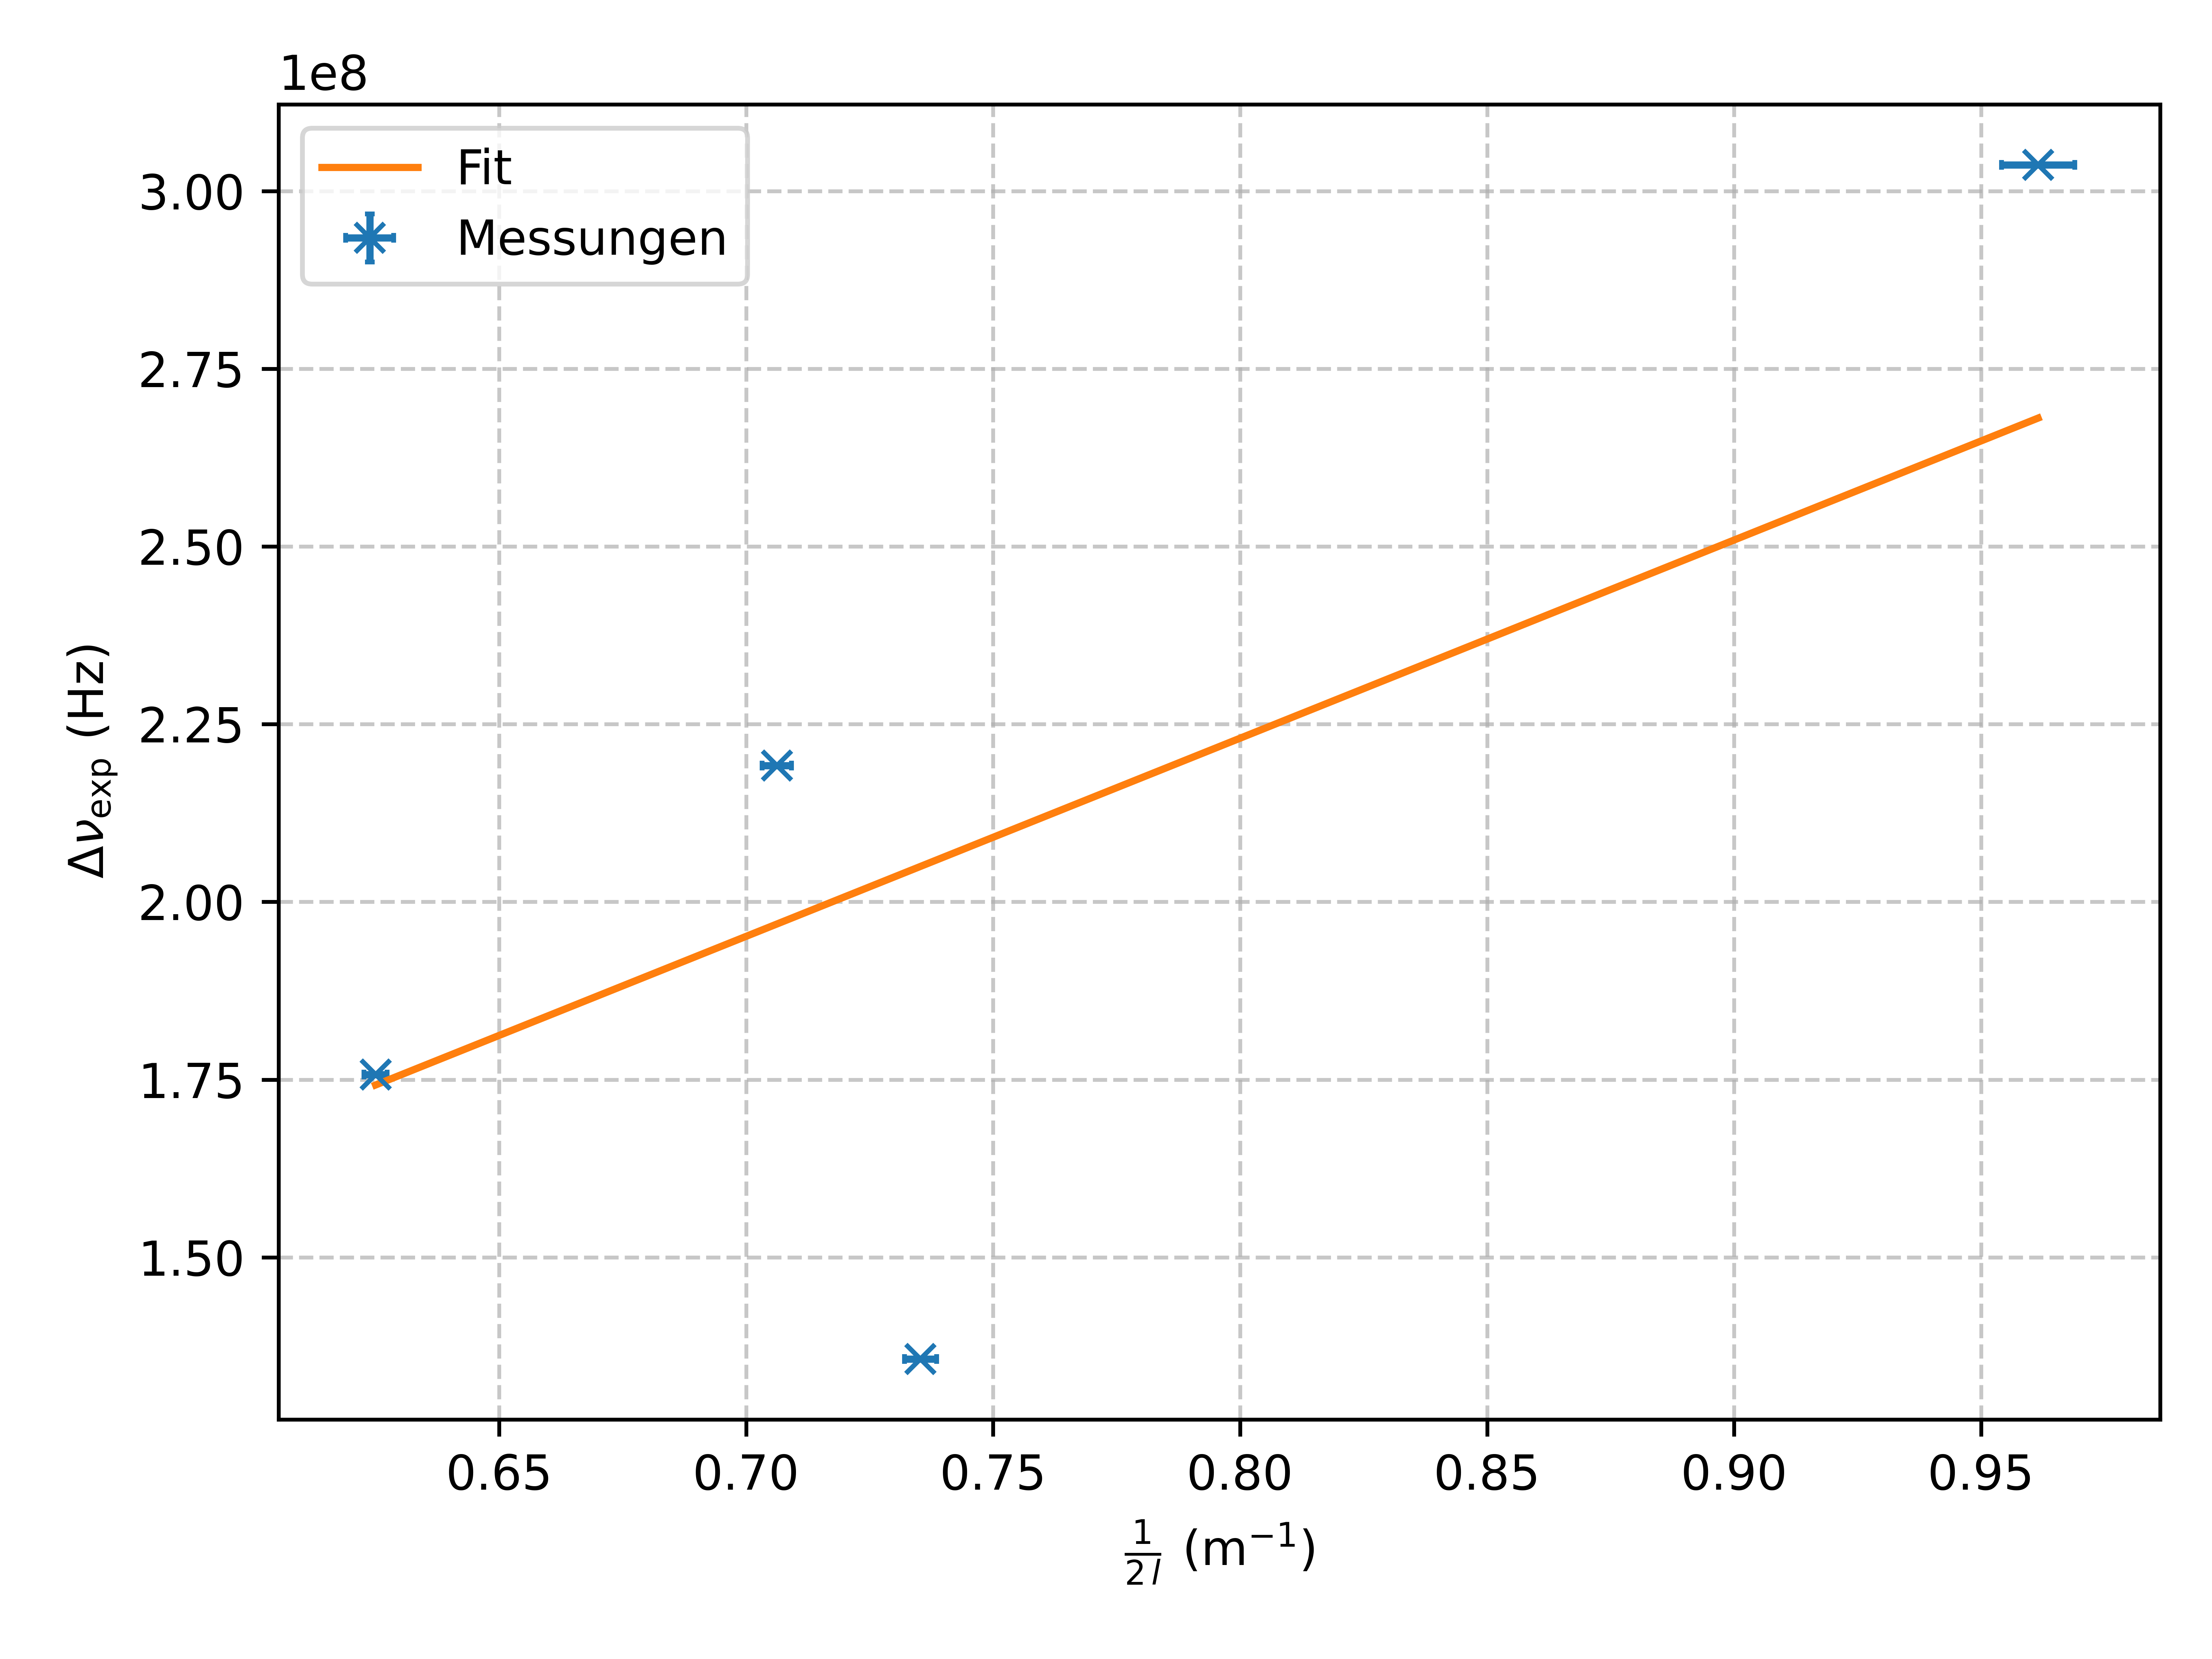
\includegraphics[width=0.75\linewidth]{light.png}
  \caption{Bestimmung der Lichtgeschwindigkeit aus den experimentellen Modenabständen \(\Delta\nu_{\mathrm{exp}}\) und den Längen \(l\) der internen He-Ne-Kavität. Die rote Linie ist die gewichtete Ausgleichsgerade, die grüne Linie ist die ideale Gerade \(c/(2l)\).}
  \label{fig:light-speed}
\end{figure}

\subsection*{Ursachen der Abweichung}

\begin{itemize}
  \item \textbf{Modenkontamination bei kurzen Längen.}  
    Bei \(l=52\,\mathrm{cm}\) und der ersten 68-cm-Messung entdeckte der konfokale Analysator nachträglich eine schwache dritte longitudinale Mode (\(\sim\!6\)\,dB unterhalb der Hauptlinien). Diese zusätzliche Mode erzeugt zwei nahe beieinanderliegende RF-Töne, deren Intensitäts-Schwerpunkt die gemessene Beat-Frequenz in Richtung höher oder niedriger verschiebt. Ergebnis: Bei 52 cm steigt \(\Delta\nu_{\mathrm{exp}}\) auf 303,7 MHz (+10 \%) statt der erwarteten 288 MHz; bei 68 cm wurde malseitig ein \(m=2\)-Beat als \(m=1\) fehlinterpretiert, wodurch 135,7 MHz (-38 \%) gemessen wurde.

  \item \textbf{Falsche Bestimmung des Harmonischen-Index \(m\).}  
    Auch nach Korrektur litt der zweite 68-cm-Durchlauf unter ungleich starken Moden, sodass die Teilung durch \(m=2\) nicht den reinen zweiten Harmonischen lieferte.

  \item \textbf{Längenunsicherheit verstärkt durch Fit-Geometrie.}  
    Maßband-Fehler von $0{,}3-0{,}4 cm$ führen in $\Delta\nu_{\mathrm{theo}}=c/(2l)$ zu $\approx 1 \%$ Abweichung; im Fit mit nur vier unabhängigen $l$ ergeben sich daraus mehrere Prozent Unsicherheit der Steigung.

  \item \textbf{Cursortechnik und Linienform.}  
    Die HWHM-Methode unterstellt eine fast Lorentzsche Peakform. Überlappende Beats erzeugen asymmetrische Linien und verschieben den Centroid um mehrere Halbwertsbreiten - weit über die nominellen \(\pm0{,}10\)\,MHz.
\end{itemize}

\subsection*{Verbesserungsvorschläge}

\begin{enumerate}
  \item \textbf{Dual-Mode Betrieb vor jedem RF-Durchgang:}  
    Den konfokalen Analysator einschleifen, so kippen, dass genau zwei gleichhohe TEM\(_{00}\)-Peaks verbleiben, und die Mechanik verriegeln. Jede IF-Spur mit Halbwertsbreite >300 kHz verwerfen.

  \item \textbf{Prüfung des Harmonischen-Index \(m\):}  
    Für jeden RF-Ton den Analysator-Snapshot heranziehen und die Anzahl der dazwischenliegenden Moden zählen, erst dann \(m=1\) oder \(m=2\) anwenden.

  \item \textbf{Metrologische Verbesserung:}  
    \emph{Längenmessung:} Kuppler auf Messschlitten (±0{,}05 cm).  
    \emph{Frequenzmessung:} IF-Signal in frequenzstabilen Zähler mit GPS-referenziertem 10 MHz-Standard (\(\delta f<0{,}001\)\,MHz) einspeisen.  
    \emph{Impedanzanpassung:} Photodiode und Mixer mit $50 \Omega$ terminieren, 6 dB-Dämpfung zur Unterdrückung von Reflexionen.

  \item \textbf{Statistik erhöhen:}  
    Mindestens acht Kavitätenlängen von 50 cm-90 cm messen. Größere Abdeckung und mehr Freiheitsgrade machen den Fit robust gegenüber Ausreißern.
\end{enumerate}

Mit gereinigtem Dual-Mode-Betrieb, Sub-kHz-Frequenzablesung und ±0{,}05 cm Längengenauigkeit sinkt die statistische Unsicherheit auf <\(1{,}5\times10^6\)\,m/s, und der gewichtete Fit konvergiert voraussichtlich zu  
$
  c_{\mathrm{opt}} = (2{,}998 \pm 0{,}003)\times10^{8}\,\mathrm{m/s},
$ 
was dem CODATA-Wert auf Promille-Ebene entspricht und die quantitative Bestätigung von \(c = 2\,l\,\Delta\nu_{\mathrm{laser}}\) abschließt.

 \chapter{Formeln: To be deleted at the end}

\section*{Spannungsteiler}

\begin{equation}
  U = \frac{R_2}{R_1 + R_2}\,U_{\mathrm{ges}}
\end{equation}

mit $U$ als Spannung am Widerstand $R_2$, $R_1$ und $R_2$ als Widerstände und $U_{\mathrm{ges}}$ als Gesamtspannung.

\section*{Energieerhaltung}

\begin{equation}
  h\,f = E_{\mathrm{kin}} + W_A,
  \quad
  E_{\mathrm{kin}} = e\,U_G
\end{equation}

mit $h$ dem Planckschen Wirkungsquantum, $f$ der Photonfrequenz, $e$ der Elementarladung, $U_G$ der Gegenspannung und $W_A$ der Austrittsarbeit.

\section*{Fehlerfortpflanzung I}

\begin{equation}
  \Delta\bigl(\sqrt{I - I_0}\bigr)
  = \sqrt{
    \Bigl(\tfrac{\Delta I}{2\,\sqrt{I - I_0}}\Bigr)^{2}
   +\Bigl(\tfrac{\Delta I_0}{2\,\sqrt{I - I_0}}\Bigr)^{2}
  }.
\end{equation}

\section*{Beugungsgitter}

\begin{equation}
  g\bigl(\sin\theta_m + \sin\beta\bigr) = m\,\lambda
  \quad\Longrightarrow\quad
  g = \frac{m\,\lambda}{\sin\theta_m + \sin\beta}
\end{equation}

\begin{equation}
  \Delta g
  = \sqrt{
    \Bigl(\tfrac{\partial g}{\partial\theta_m}\,\Delta\theta_m\Bigr)^{2}
   +\Bigl(\tfrac{\partial g}{\partial\beta}\,\Delta\beta\Bigr)^{2}
  }.
\end{equation}

\begin{equation}
  \frac{\partial g}{\partial\theta_m}
  = \frac{m\,\lambda\,\cos\theta_m}{(\sin\theta_m + \sin\beta)^{2}},
  \quad
  \frac{\partial g}{\partial\beta}
  = \frac{m\,\lambda\,\cos\beta}{(\sin\theta_m + \sin\beta)^{2}}.
\end{equation}

\section*{Mittelwert der Gitterkonstante}

\begin{equation}
  \overline{g}
  = \frac{\sum_{i=1}^{N} \bigl(g_i/\Delta g_i\bigr)}
         {\sum_{i=1}^{N} \bigl(1/\Delta g_i\bigr)},
  \quad
  \Delta\overline{g}
  = \sqrt{\frac{N}{\sum_{i=1}^{N} 1/(\Delta g_i)^{2}}}\,.
\end{equation}

\section*{Isotopenverhältnis}

\begin{equation}
  \lambda = g\,(\sin\theta_m + \sin\beta),
  \quad
  \frac{\partial\lambda}{\partial\beta} = g\,\cos\beta,
  \quad
  \Delta\beta \approx \frac{d}{f}.
\end{equation}

\section*{Fehlerfortpflanzung II}

\begin{equation}
  \Delta\lambda
  = \sqrt{
      \Bigl(\tfrac{\lambda}{g}\,\Delta g\Bigr)^{2}
    + \Bigl(g\,\cos\alpha\,\Delta\alpha\Bigr)^{2}
    + \Bigl(g\,\cos\beta\,\Delta\beta\Bigr)^{2}
  }.
\end{equation}

\begin{equation}
  \Delta(\Delta\lambda)
  = \sqrt{
      \Bigl(\tfrac{d\,\cos\beta}{f}\,\Delta g\Bigr)^{2}
    + \Bigl(\tfrac{-d\,\sin\beta}{f\,g}\,\Delta\beta\Bigr)^{2}
    + \Bigl(\tfrac{g\,\cos\beta}{f}\,\Delta d\Bigr)^{2}
  }.
\end{equation}

\section*{Balmer‐Formel}

\begin{equation}
  \frac{1}{\lambda}
  = R_H\Bigl(\tfrac{1}{2^{2}} - \tfrac{1}{n^{2}}\Bigr),
  \quad n=3,4,5,\dots
\end{equation}

\begin{equation}
  R_H
  = \frac{1/\lambda}{\bigl(\tfrac{1}{4} - \tfrac{1}{n^{2}}\bigr)},
  \quad
  \Delta R_H
  = \frac{\Delta\lambda}{\lambda^{2}\,\bigl(\tfrac{1}{4} - \tfrac{1}{n^{2}}\bigr)}.
\end{equation}

\section*{Plancksches Wirkungsquantum}

\begin{equation}
  h
  = \Bigl(\tfrac{m_e\,e^{4}}{8\,\varepsilon_{0}^{2}\,c\,R_H}\Bigr)^{1/3},
  \quad
  \Delta h
  = \frac{1}{3}
    \Bigl(\tfrac{m_e\,e^{4}}{8\,\varepsilon_{0}^{2}\,c}\Bigr)^{1/3}
    R_H^{-4/3}\,\Delta R_H.
\end{equation}

 \chapter{Fazit}
In diesem Experiment wurde der Umgang mit einem Rastertunnelmikroskop erfolgreich erlernt. Eine Goldprobe und eine HOPG-Probe wurden analysiert. Ziel der Untersuchung der Goldprobe war die Erstellung hochwertiger Bilder, die die Oberflächenstruktur der Probe detailliert beschreiben – ein Ziel, das erfolgreich erreicht/nicht erfolgreich erreicht wurde. Anschließend wurde die HOPG-Probe analysiert, bei welchen eine atomare Auflösung erreicht werden sollte. Diese Analyse verlief erfolgreich/nicht erfolgreich, sodass die durchschnittlichen Bindungswinkel und Atomabstände der Kohlenstoffatome aus den erhaltenen Bildern bestimmt werden konnten/nur annähernd bestimmt werden konnten.
Die Messungen ergaben einen durchschnittlichen Bindungswinkel von ( ± )° und einen durchschnittlichen Atomabstand von ( ± ) [Einheit]. Obwohl der ermittelte Bindungswinkel weitgehend mit den Literaturwerten übereinstimmt/nicht übereinstimmt, weist der durchschnittliche Atomabstand eine signifikante/kleine Abweichung auf. Eine mögliche Fehlerquelle ist eine ungenaue Kalibrierung der Piezoelemente im STM. Eine perspektivische Verzerrung, die durch die Neigung der Gitterebene der Probe verursacht wird, könnte ebenfalls zu Abweichungen geführt haben. Daher sind zusätzliche Kalibrierungsmessungen mit dem Gerät erforderlich, um die Genauigkeit der Ergebnisse zu verbessern.
 \chapter{Anhang}
\section{Abbildungen}
\subsection*{Photoeffekt}
\subsection*{Balmer Serie}

\begin{figure}[H]
\centering
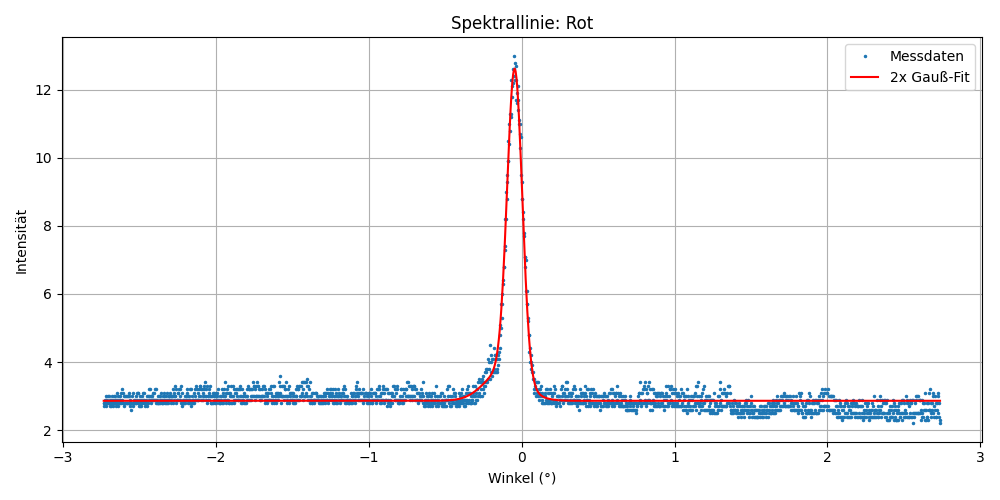
\includegraphics[width=0.7\linewidth]{figs/dt_rot_155_62.png}
\caption{Gaußfit für $H_\alpha$ mit $\chi_{red} = 0.06$}
\label{fig:H_a}
\end{figure}

\begin{figure}[H]
\centering
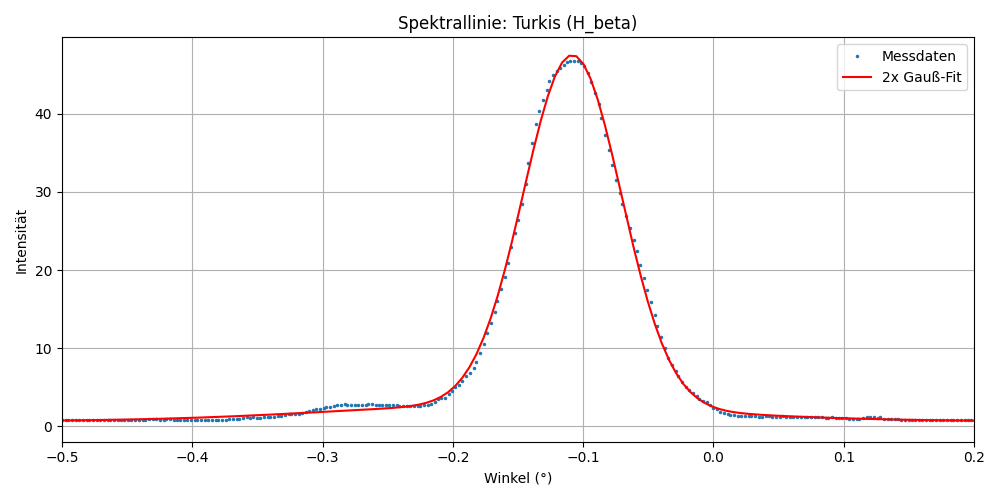
\includegraphics[width=0.7\linewidth]{figs/dt_turkis_145_55_5.png}
\caption{Gaußfit für $H_\beta$ mit $\chi_{red} = 0.06$}
\label{fig:H_b}
\end{figure}

\begin{figure}[H]
\centering
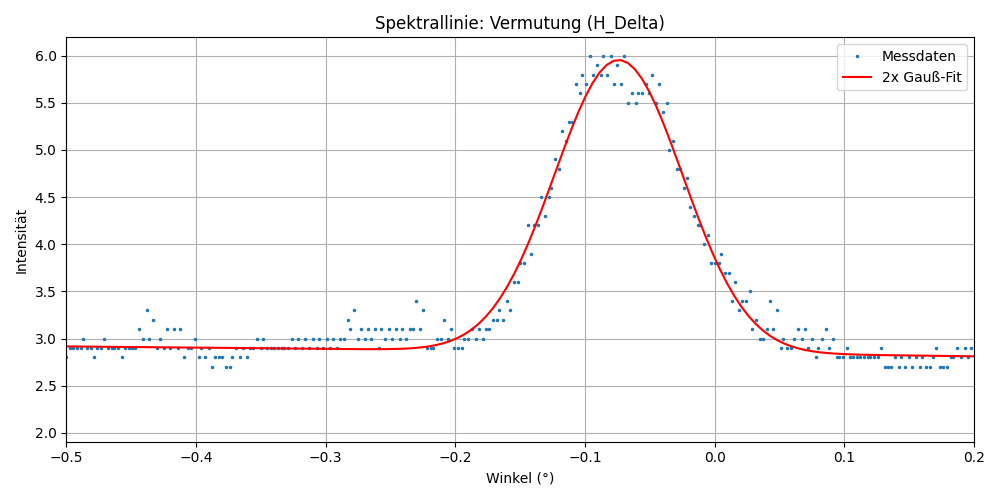
\includegraphics[width=0.7\linewidth]{figs/dt_vermutung_145_49.png}
\caption{Gaußfit für die Vermutete Linie $H_\delta$ mit $\chi_{red} = 0.03$}
\label{fig:H_d}
\end{figure}


\begin{figure}[H]
  \centering
  \begin{minipage}[t]{\textwidth}
    \centering
    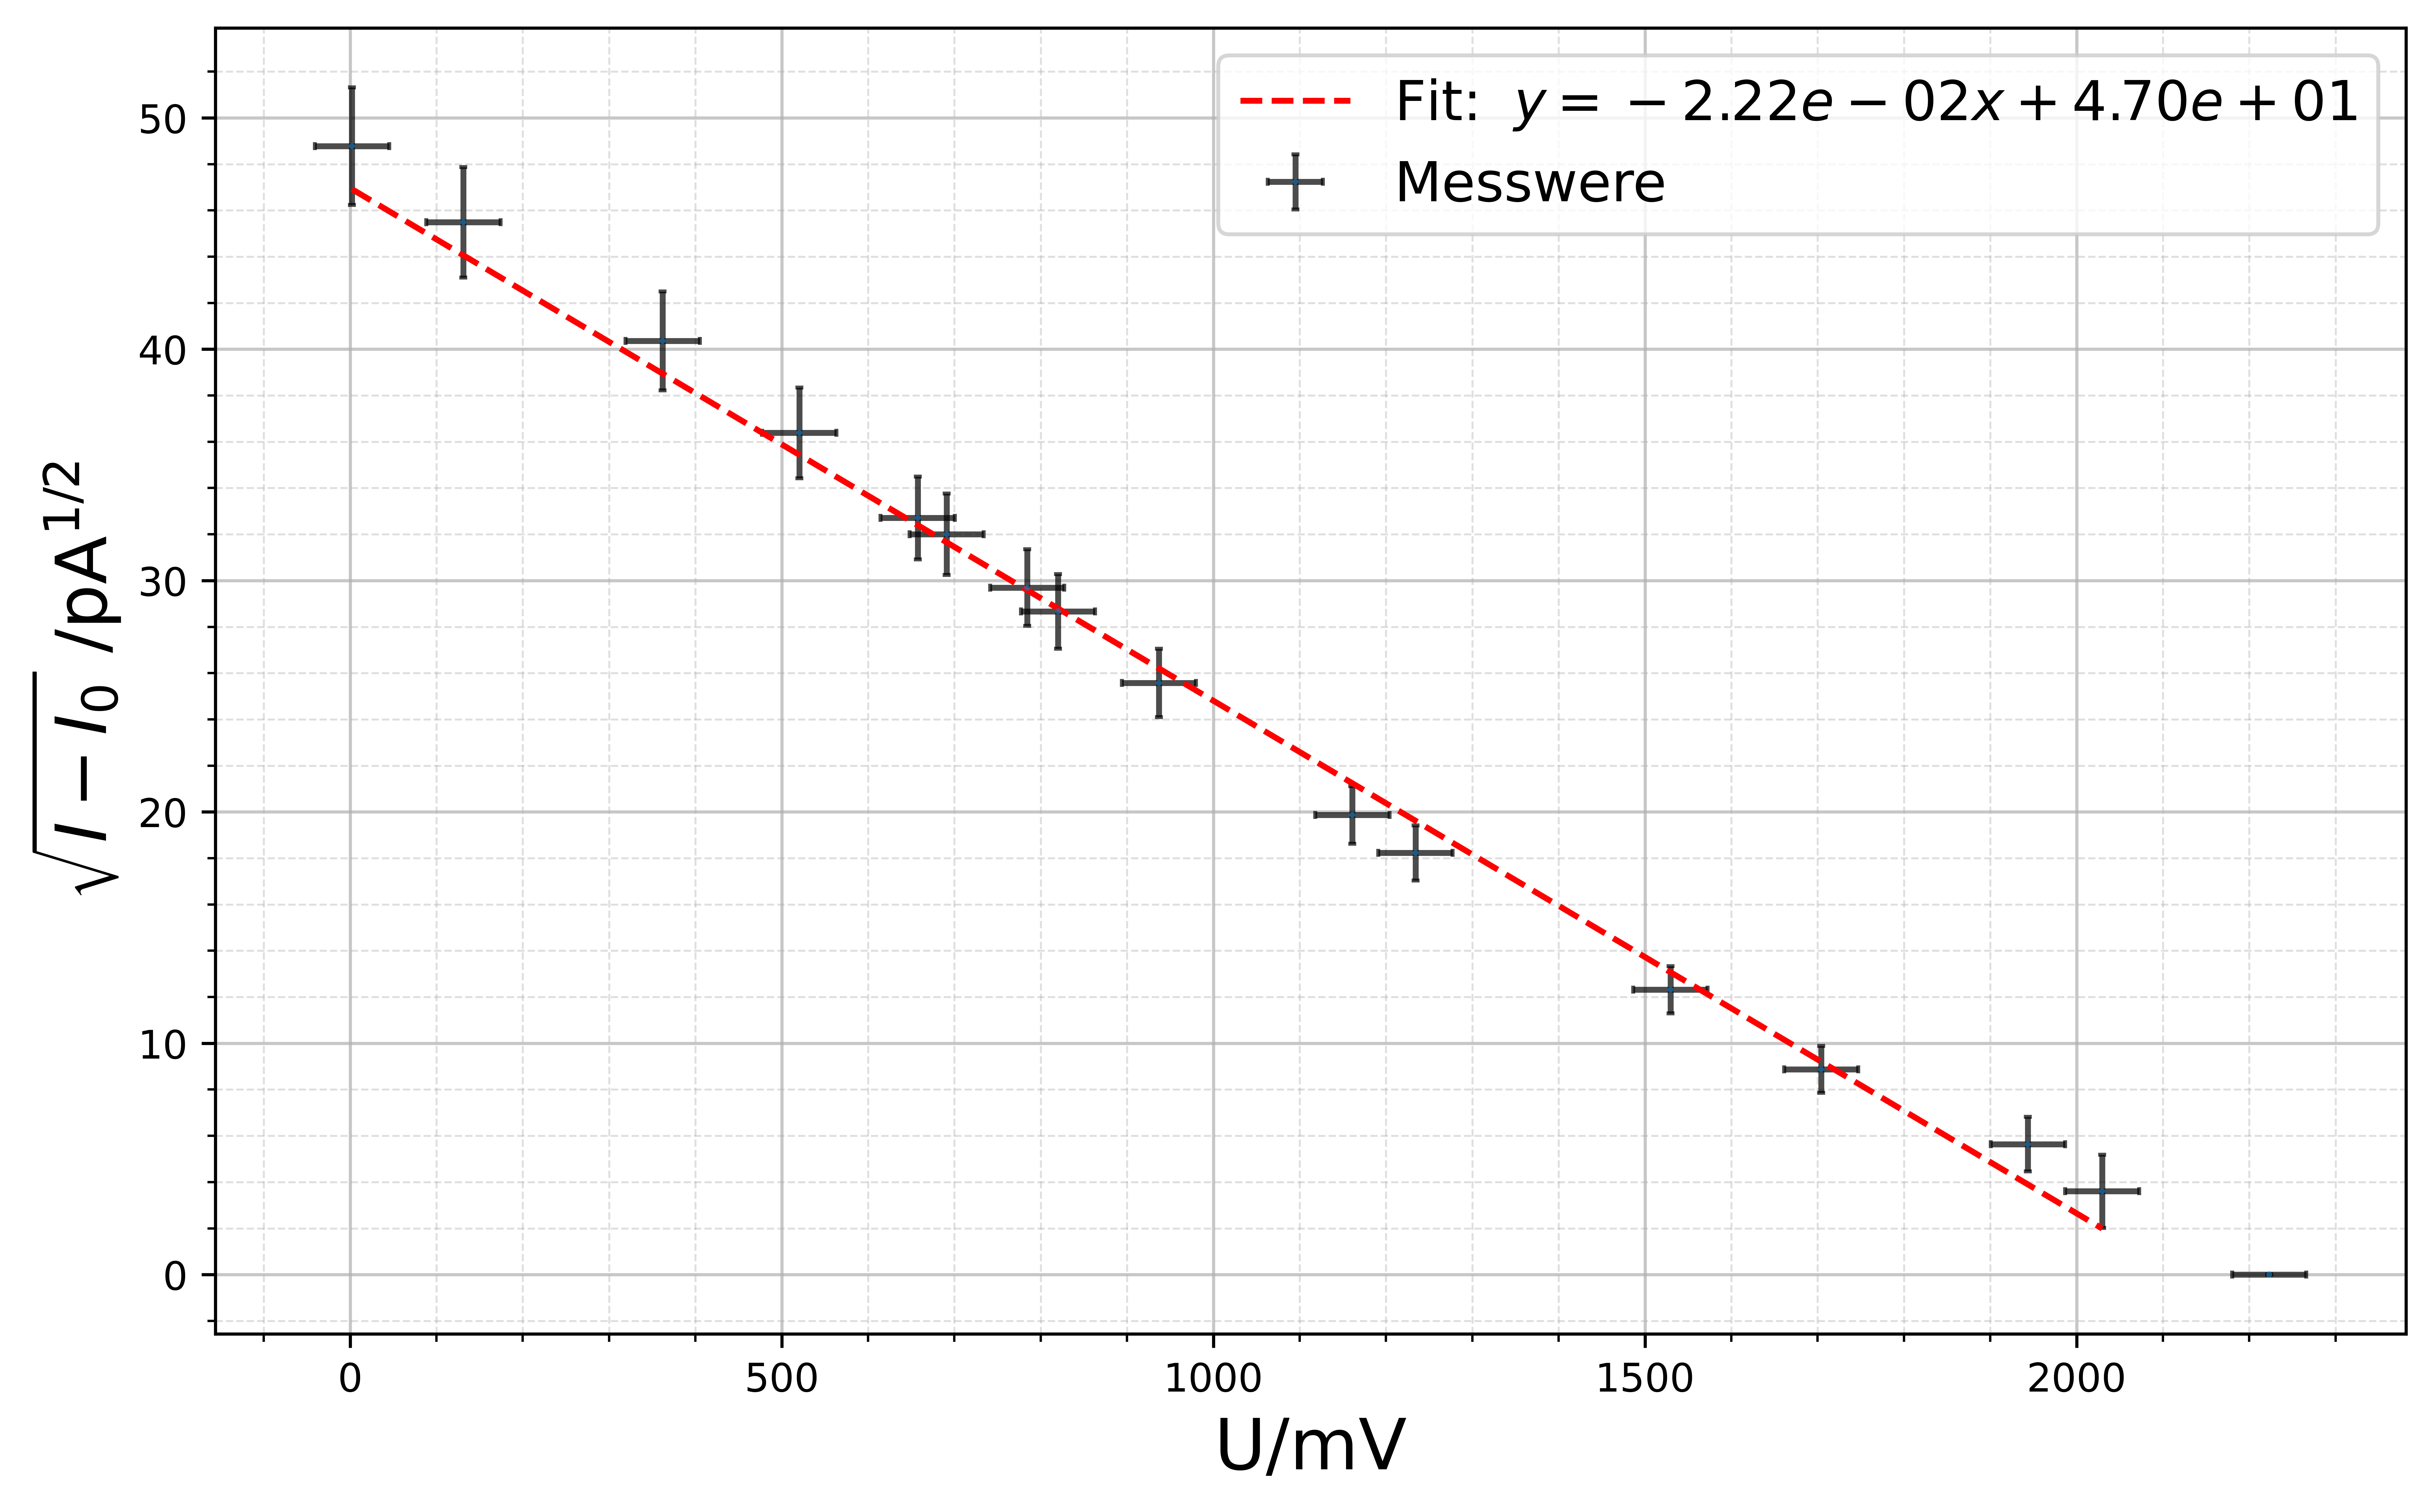
\includegraphics[width=0.95\linewidth]{figs/365_1.png}
    \captionof{figure}{Messung 1 bei $\lambda=\SI{365}{\nm}$. Die Werte und Unsicherheiten sind in ~\cref{tab:365_first}.}
    \label{fig:365_first}
  \end{minipage}\hfill
  \begin{minipage}[t]{\textwidth}
    \centering
    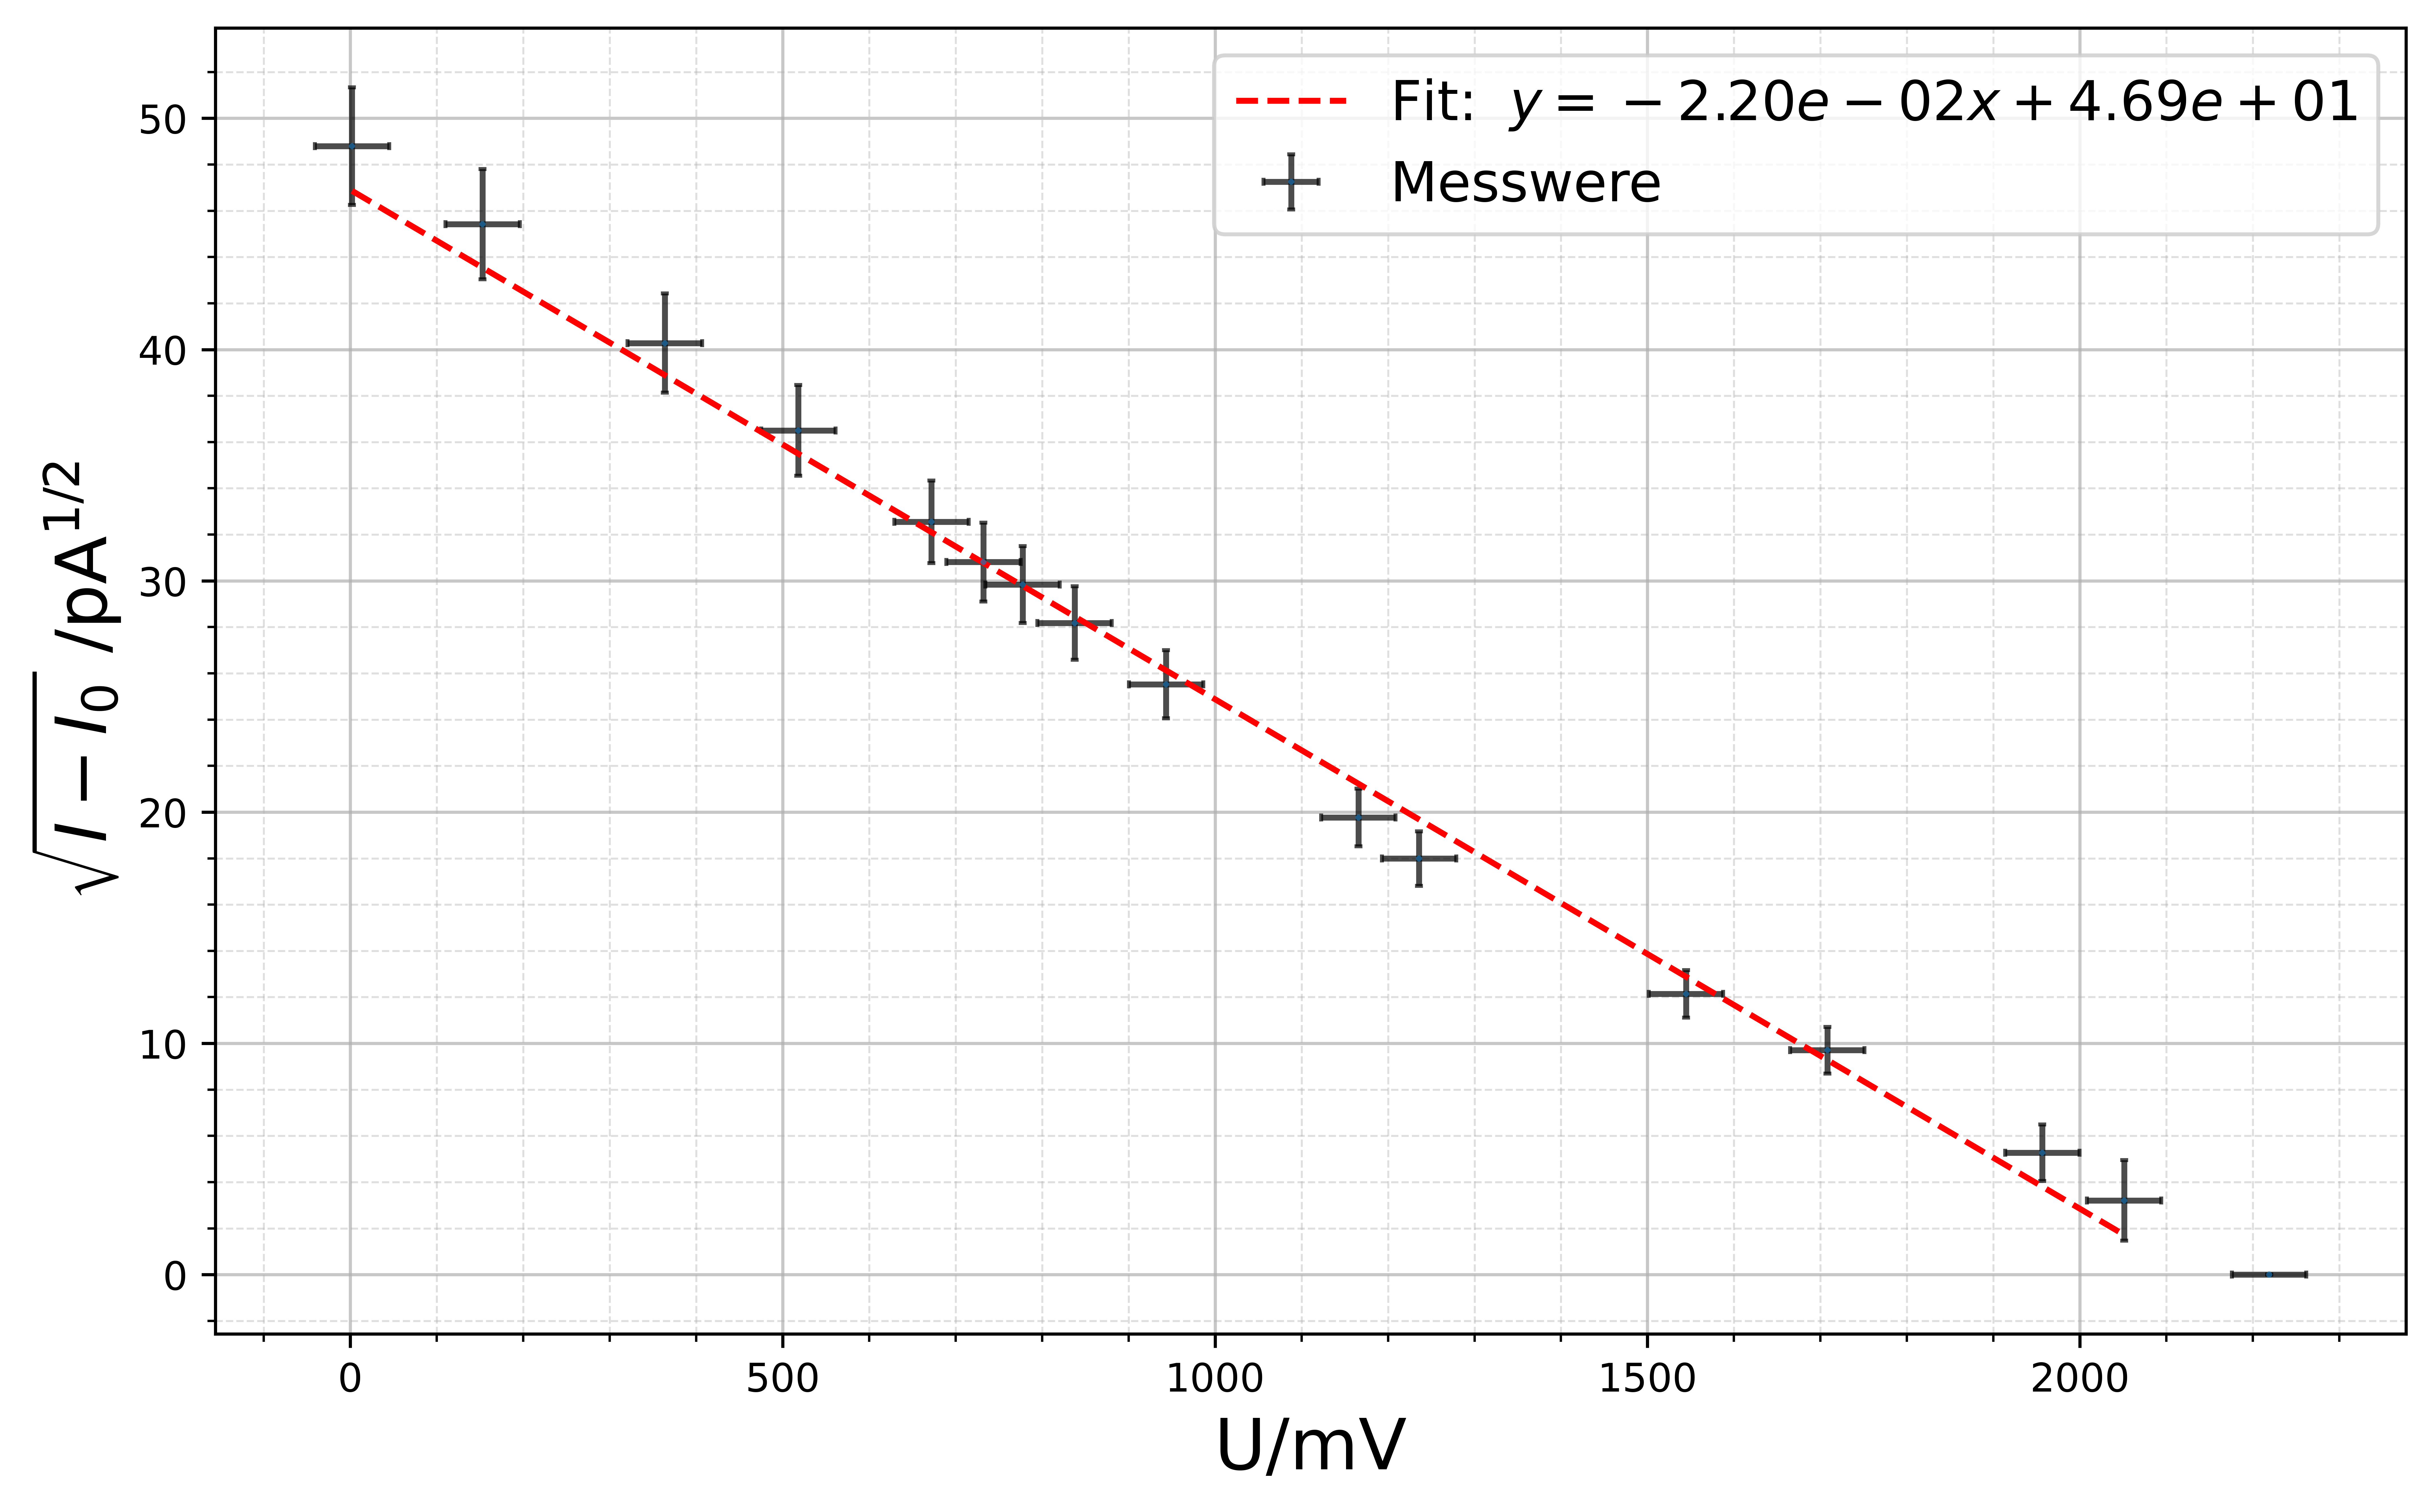
\includegraphics[width=0.95\linewidth]{figs/365_2.png}
    \captionof{figure}{Messung 2 bei $\lambda=\SI{365}{\nm}$. Die Werte und Unsicherheiten sind in ~\cref{tab:365_second}.}
    \label{fig:365_second}
  \end{minipage}\hfill
\end{figure}
\vfil
\begin{figure}[H]
  \centering
  \begin{minipage}[t]{\linewidth}
    \centering
    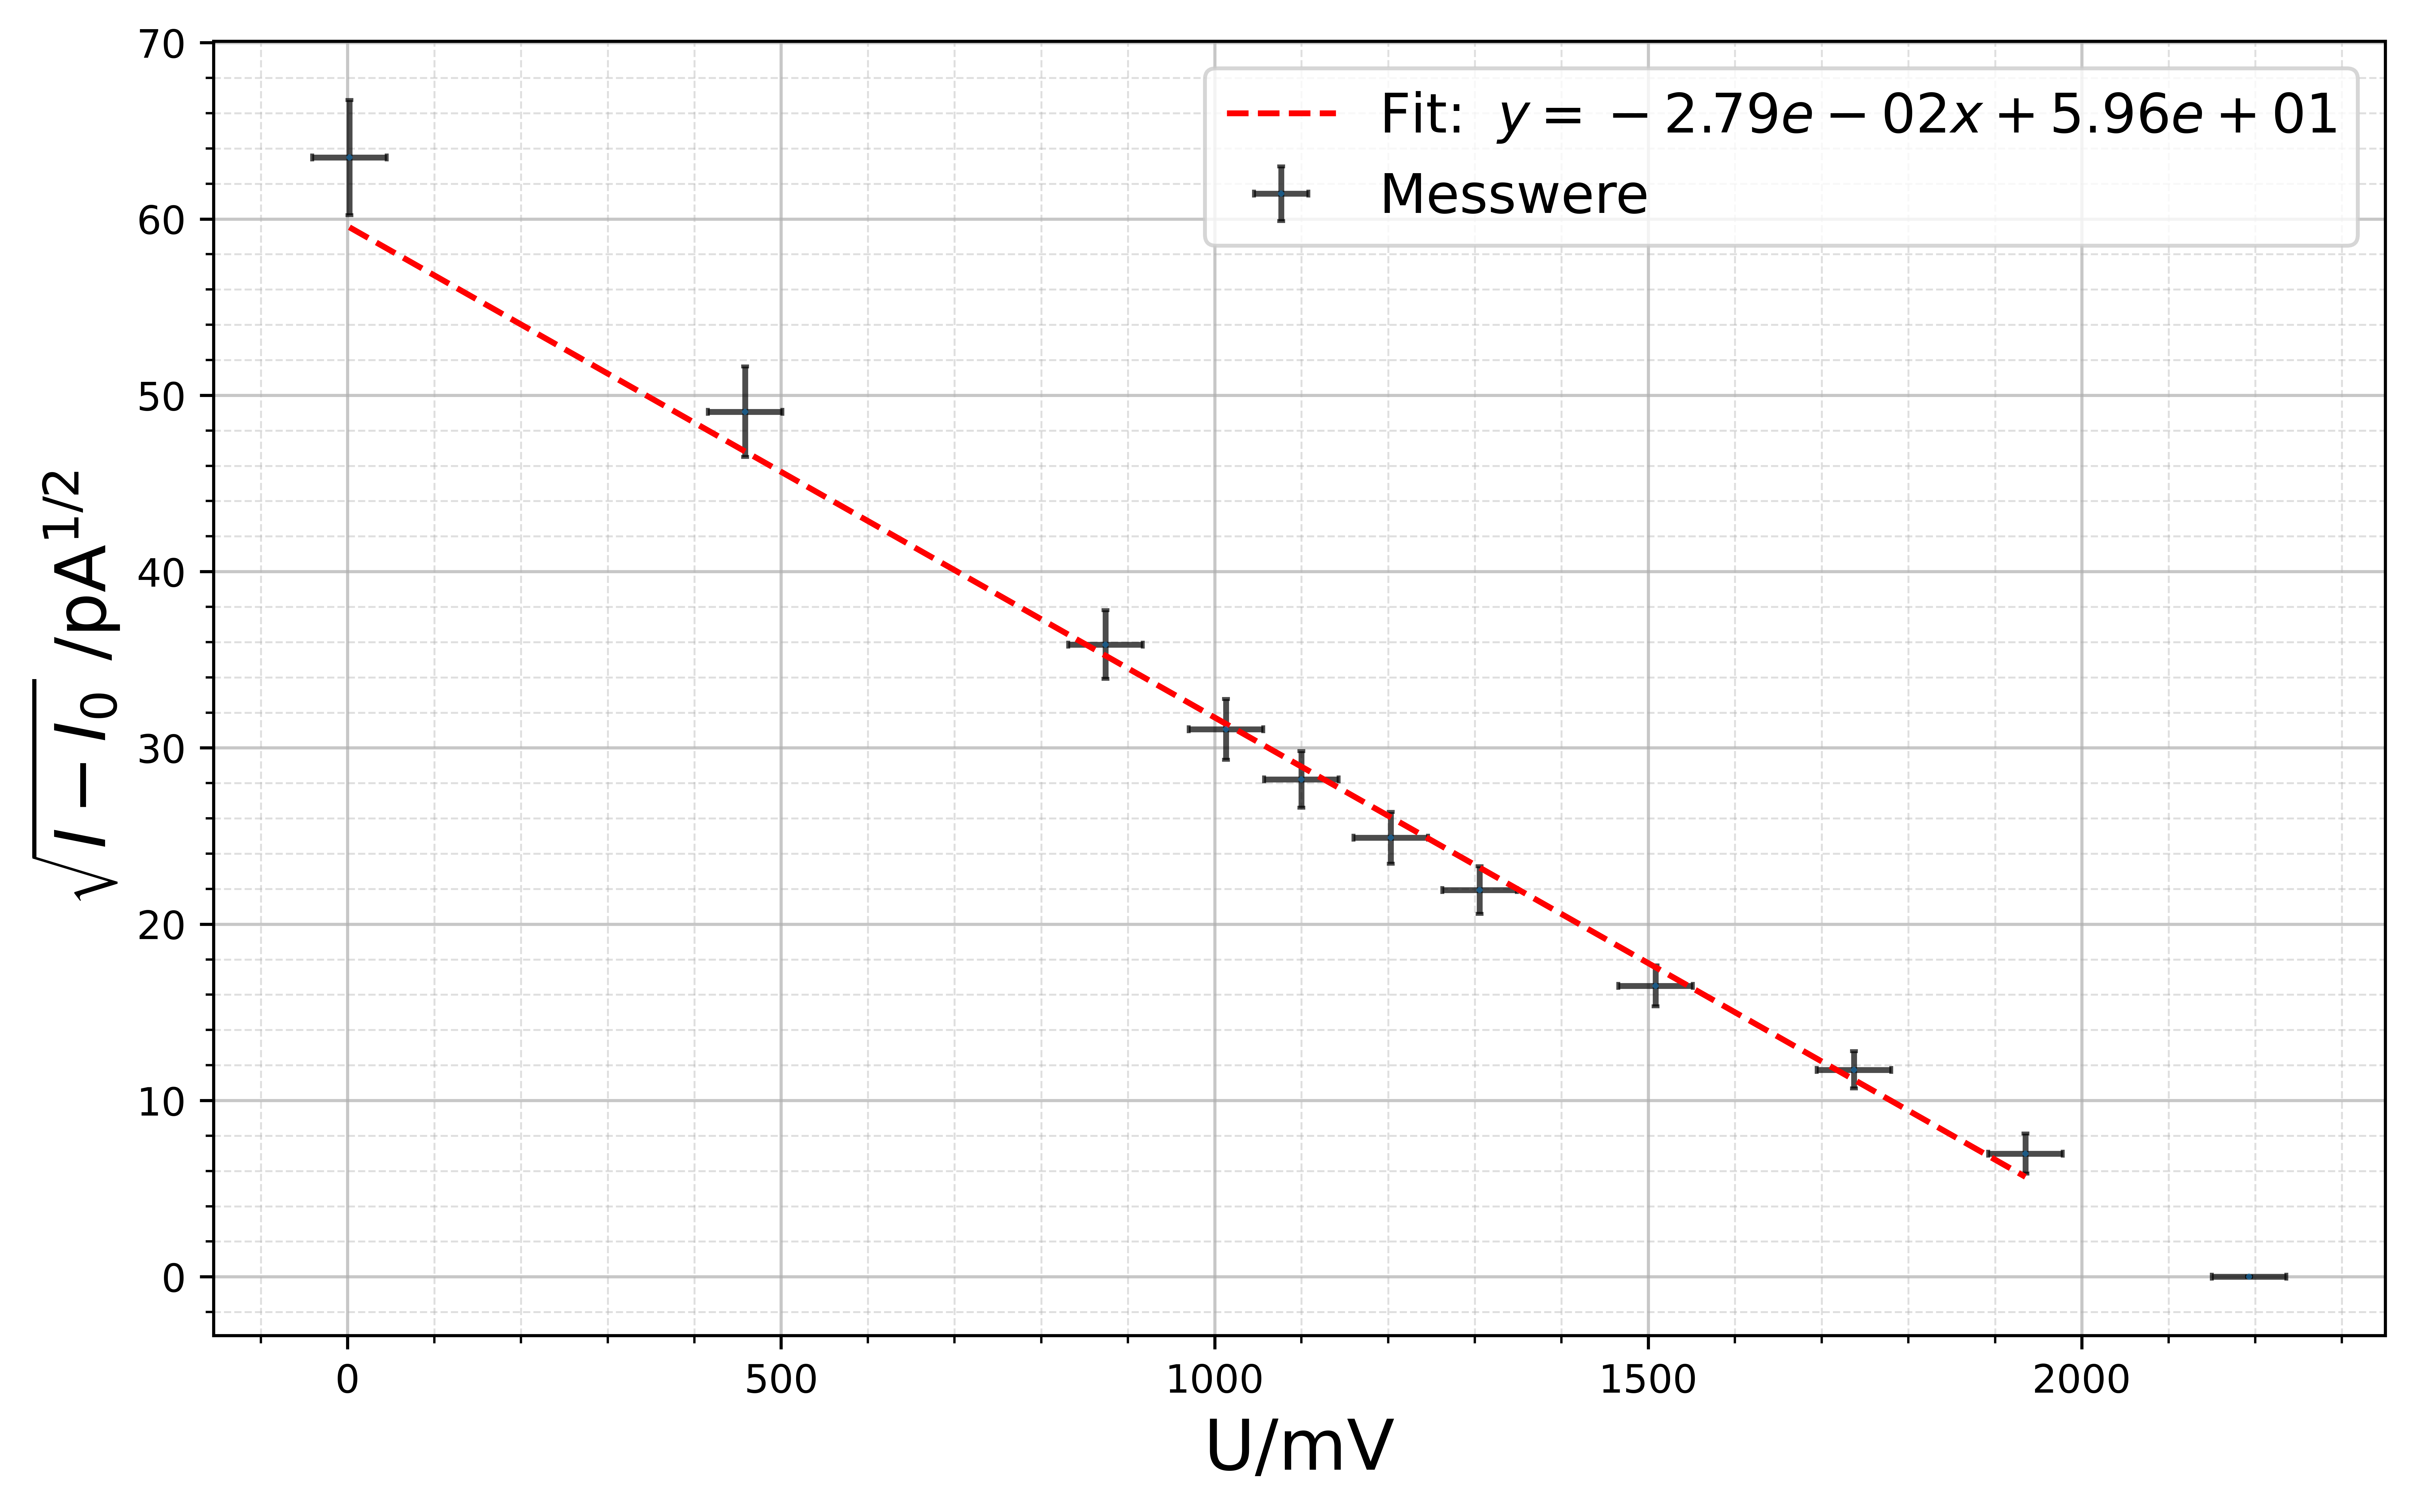
\includegraphics[width=0.95\linewidth]{figs/365_50.png}
    \captionof{figure}{Messung bei $50\%$ Intensität und $\lambda=\SI{365}{\nm}$. 
    Die Werte und Unsicherheiten sind in \cref{tab:365_50pct}.%
    }
    \label{fig:365_50}
  \end{minipage}\hfill
  \begin{minipage}[t]{\linewidth}
    \centering
    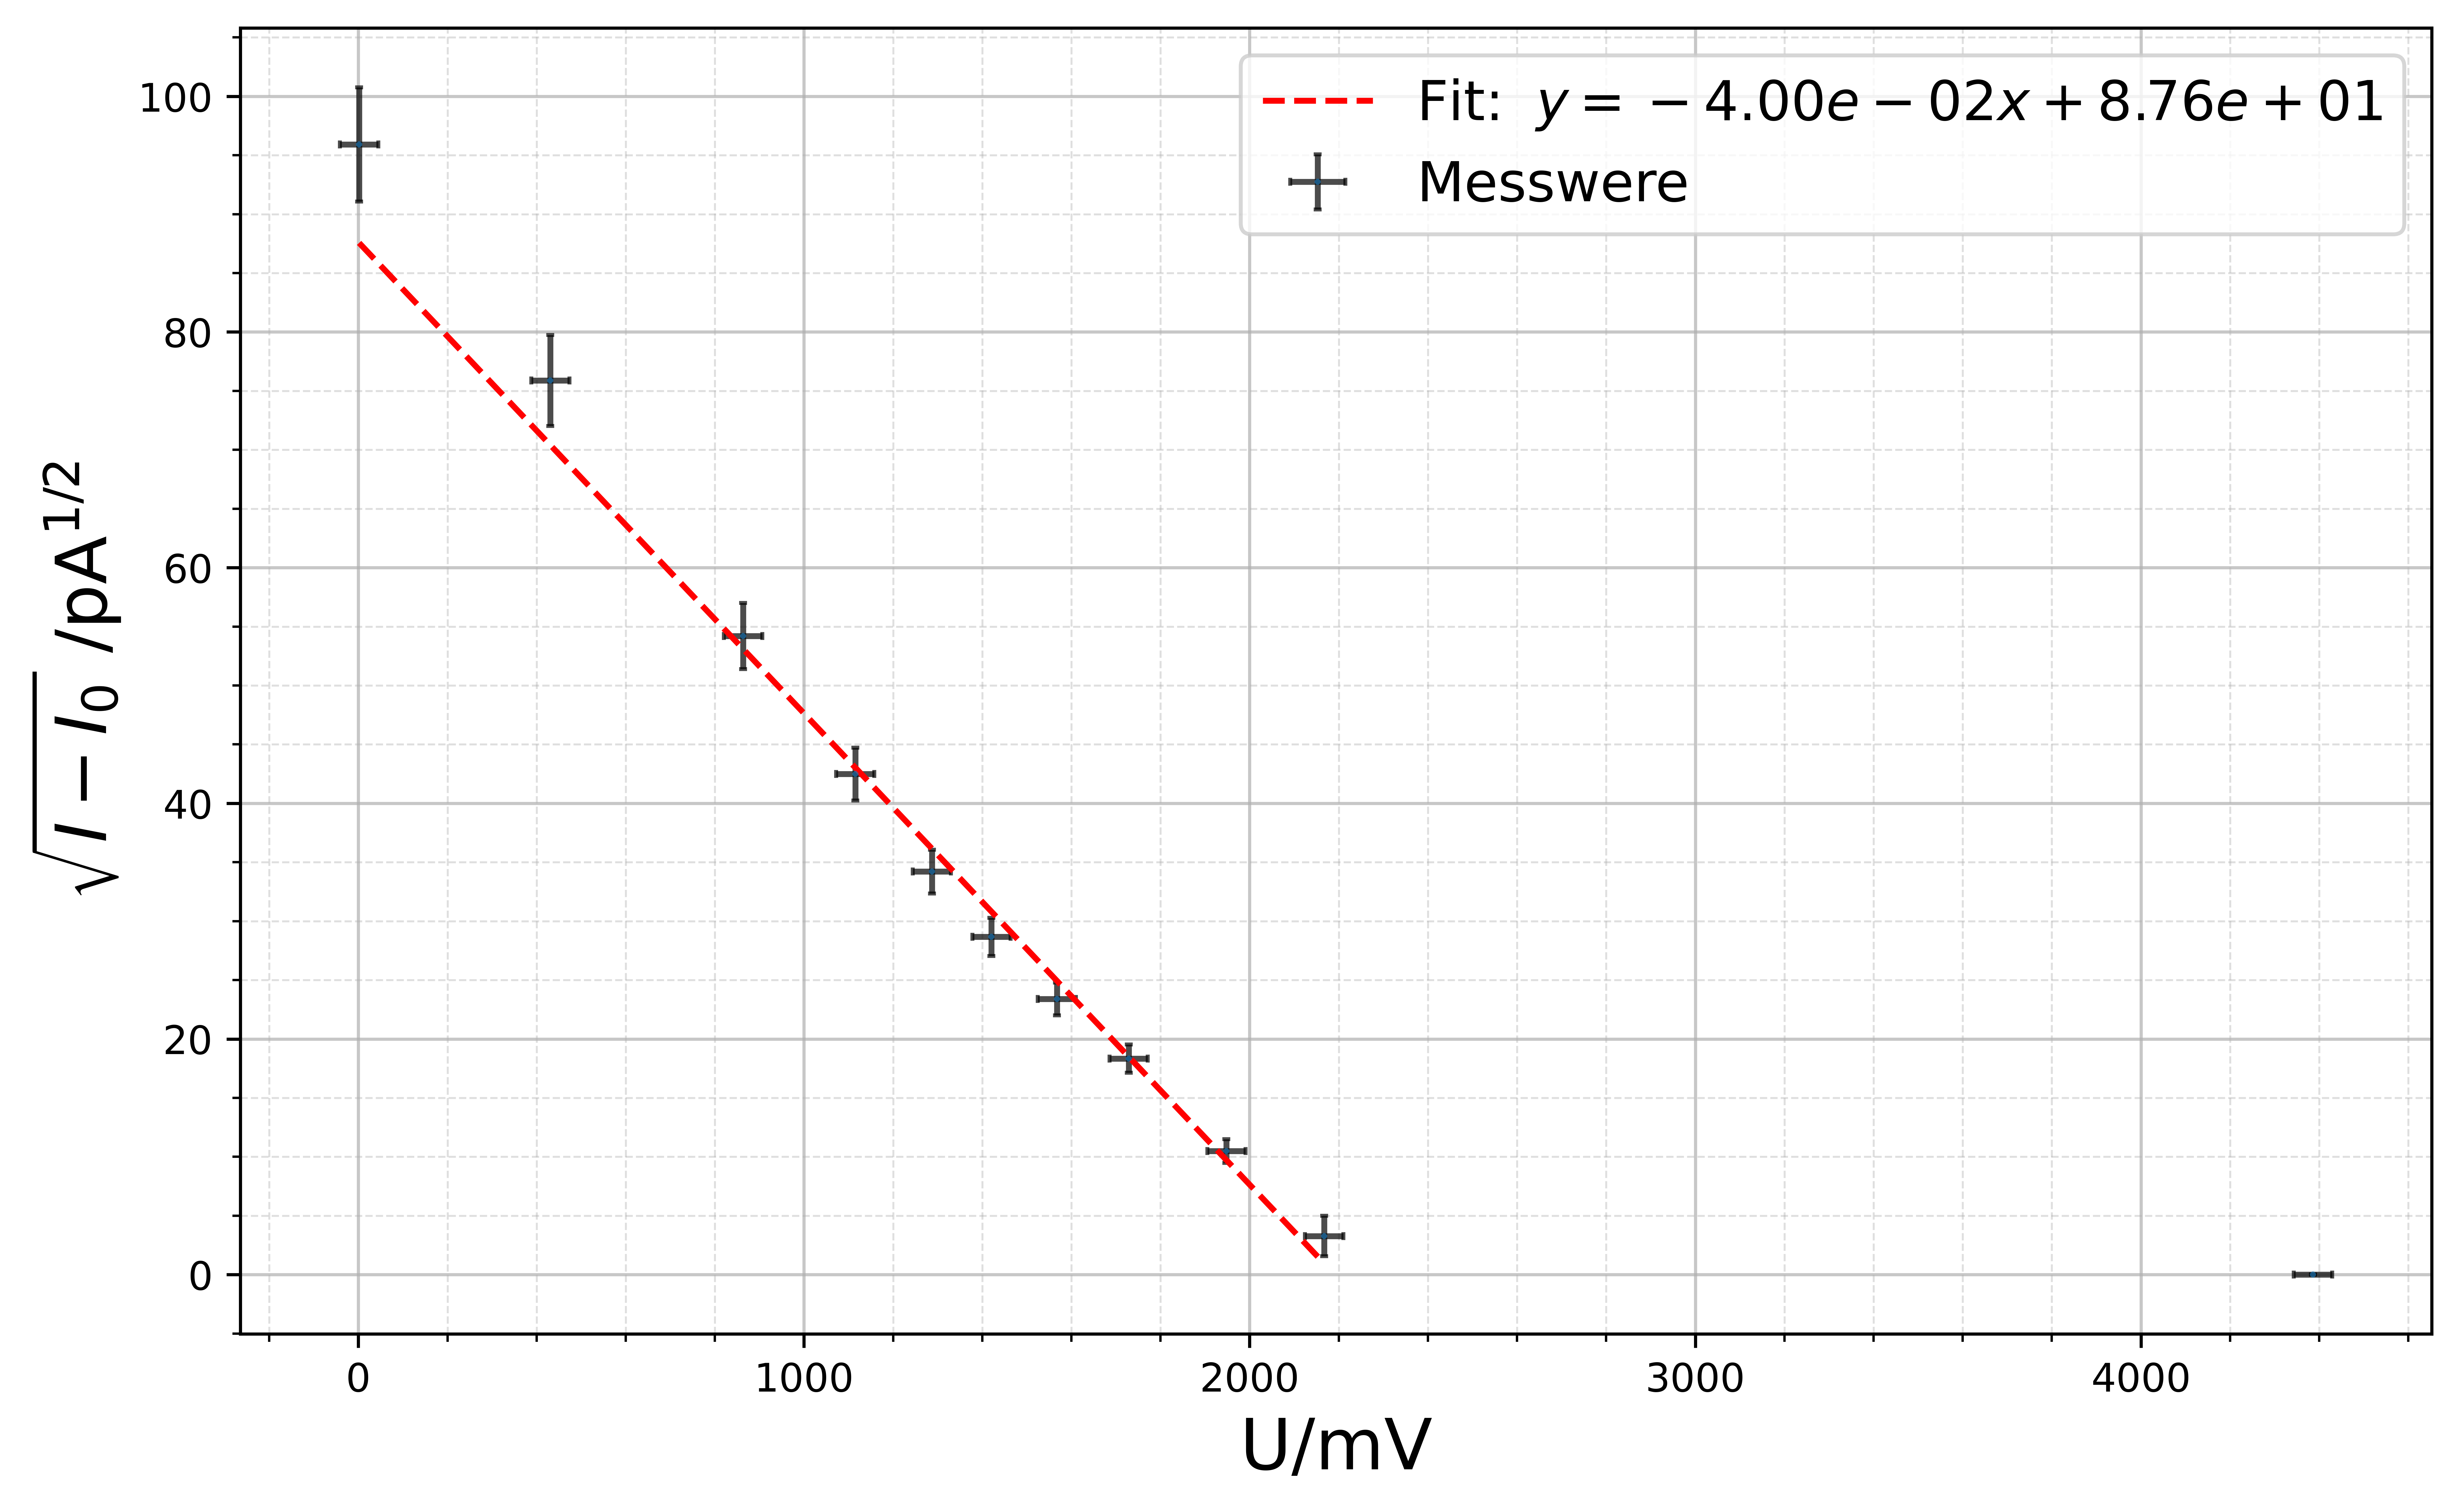
\includegraphics[width=0.95\linewidth]{figs/365_max.png}
    \captionof{figure}{%
      Messung bei maximaler Intensität und $\lambda=\SI{365}{\nm}$. 
      Die Werte und Unsicherheiten sind in \cref{tab:365_max}.%
    }
    \label{fig:365_max}
  \end{minipage}
\end{figure}

\begin{figure}[H]
  \centering
  \begin{minipage}[t]{\linewidth}
    \centering
    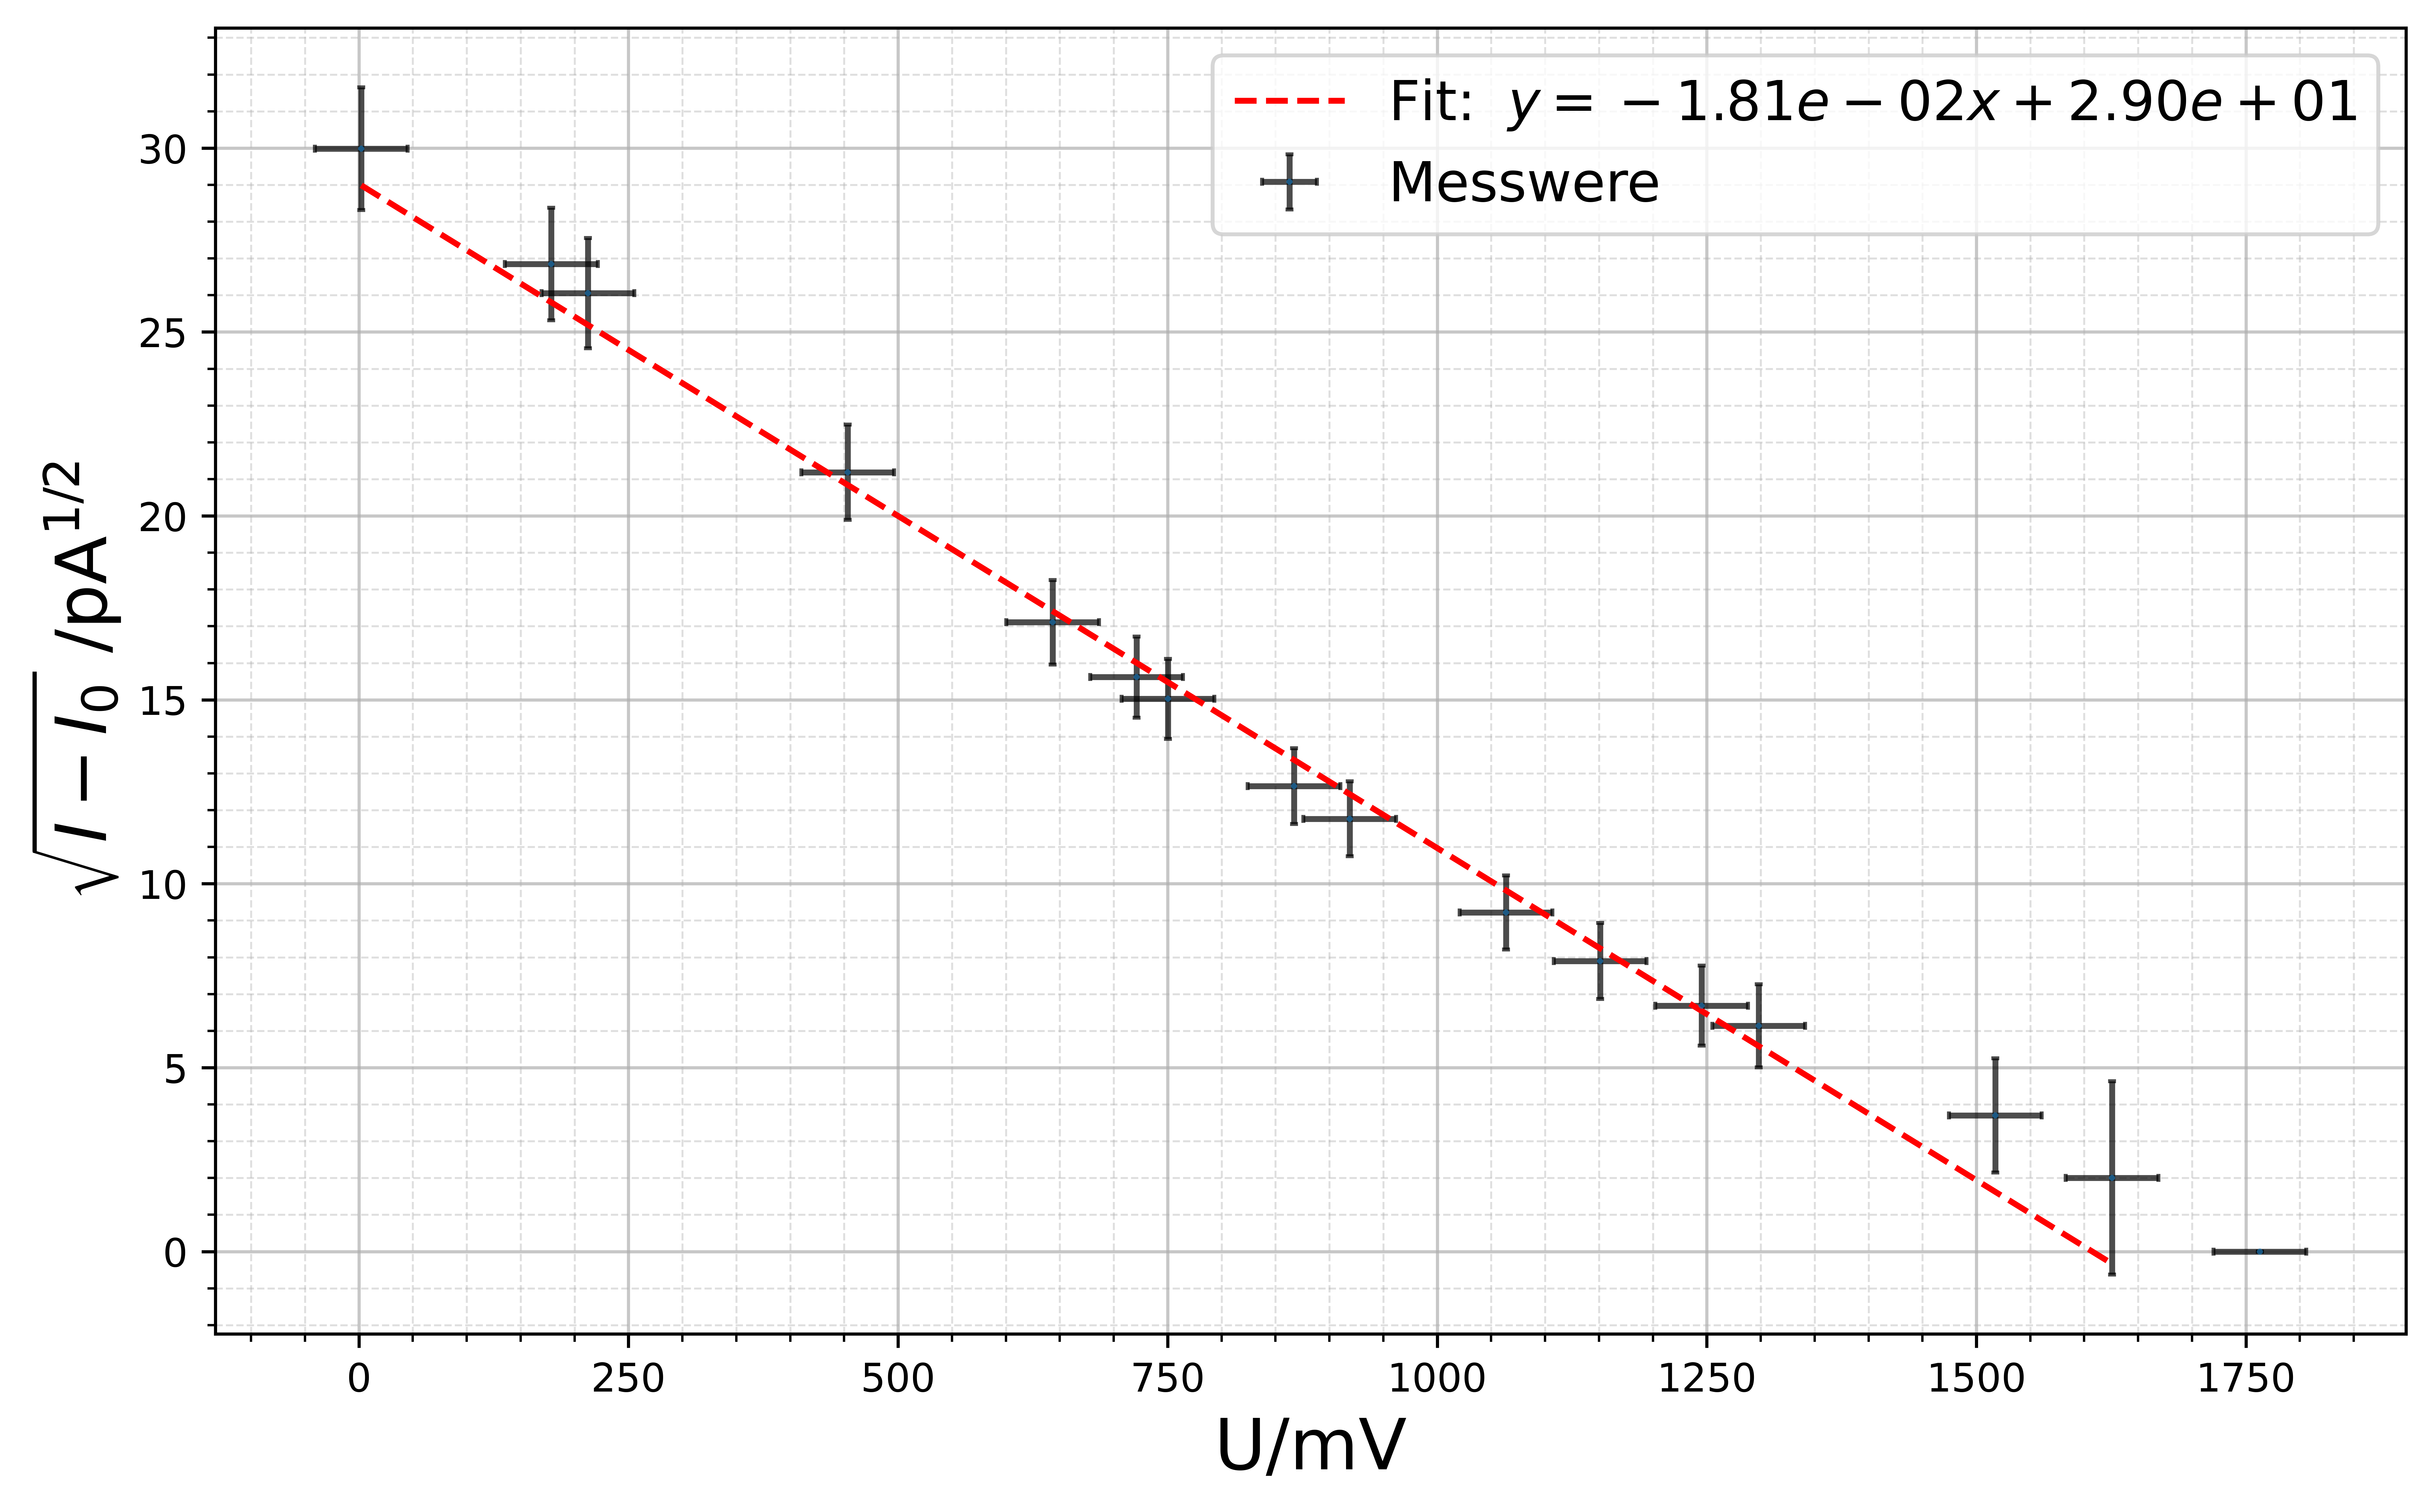
\includegraphics[width=0.95\linewidth]{figs/405_1.png}
    \captionof{figure}{%
      Messung 1 bei $\lambda=\SI{405}{\nm}$. 
      Die Werte und Unsicherheiten sind in \cref{tab:405_first}.%
    }
    \label{fig:405_first}
  \end{minipage}\hfill
  \begin{minipage}[t]{\linewidth}
    \centering
    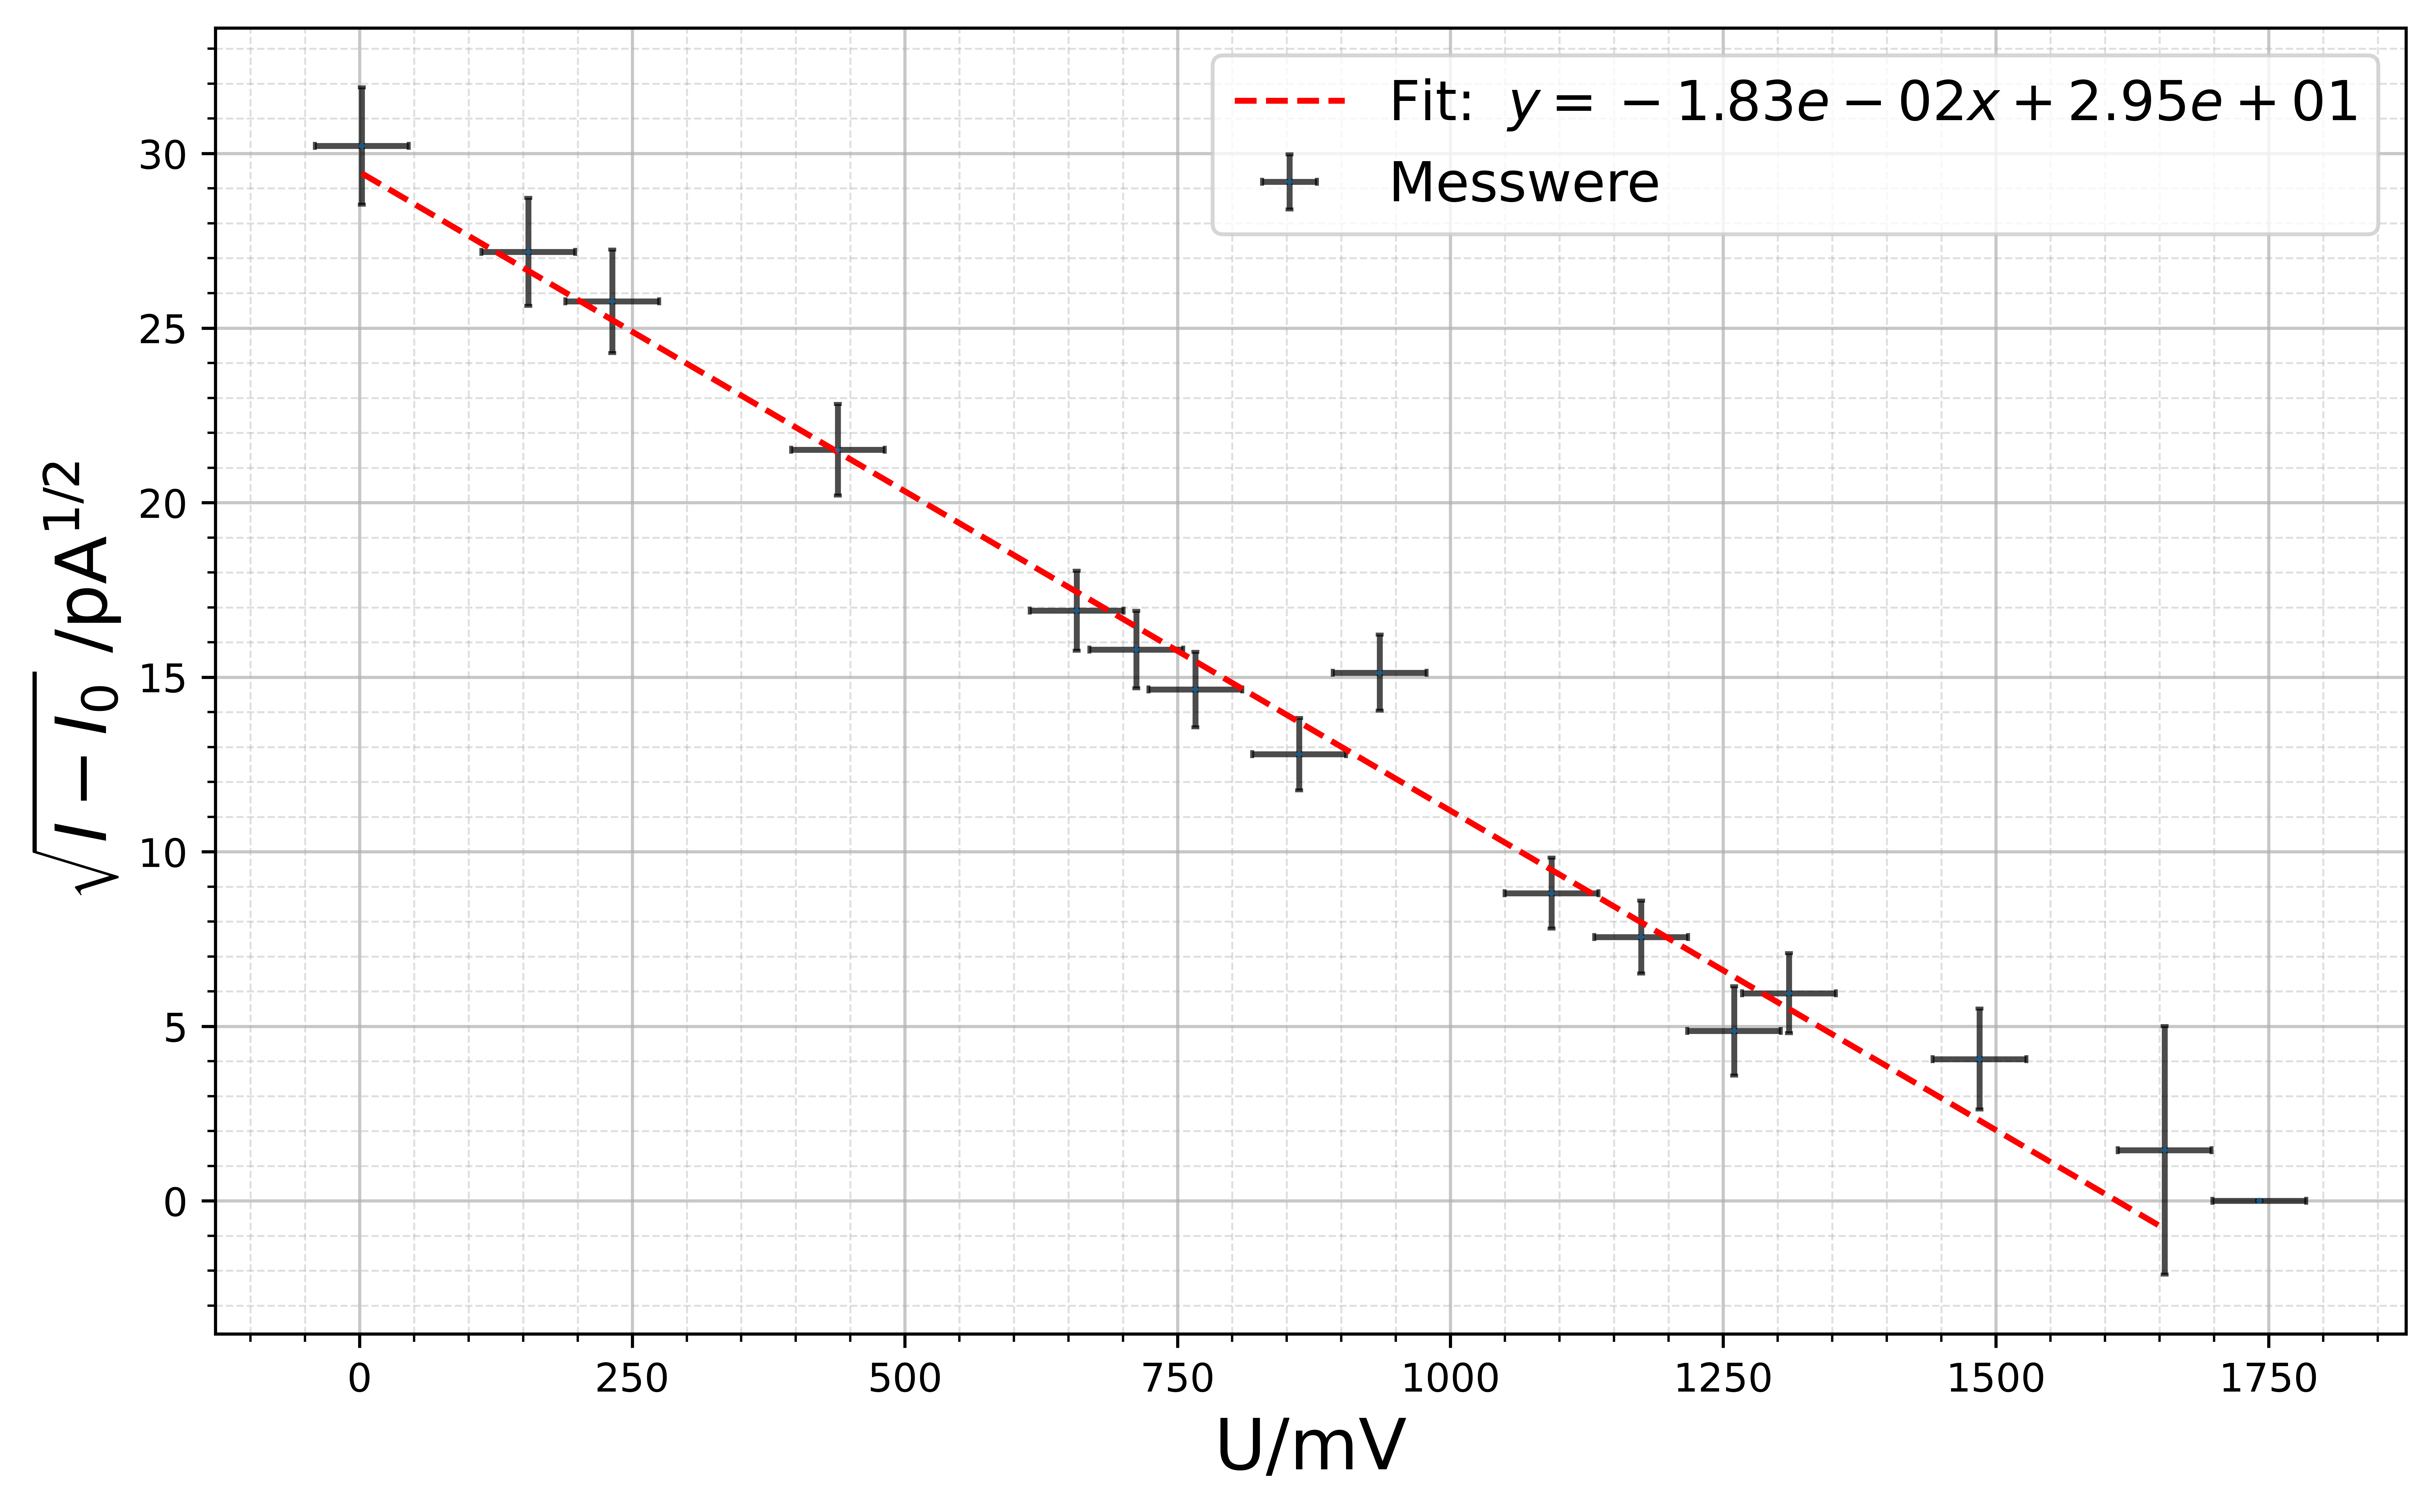
\includegraphics[width=0.95\linewidth]{figs/405_2.png}
    \captionof{figure}{%
      Messung 2 bei $\lambda=\SI{405}{\nm}$. 
      Die Werte und Unsicherheiten sind in \cref{tab:405_second}.%
    }
    \label{fig:405_second}
  \end{minipage}
\end{figure}

\begin{figure}[H]
  \centering
  \begin{minipage}[t]{\linewidth}
    \centering
    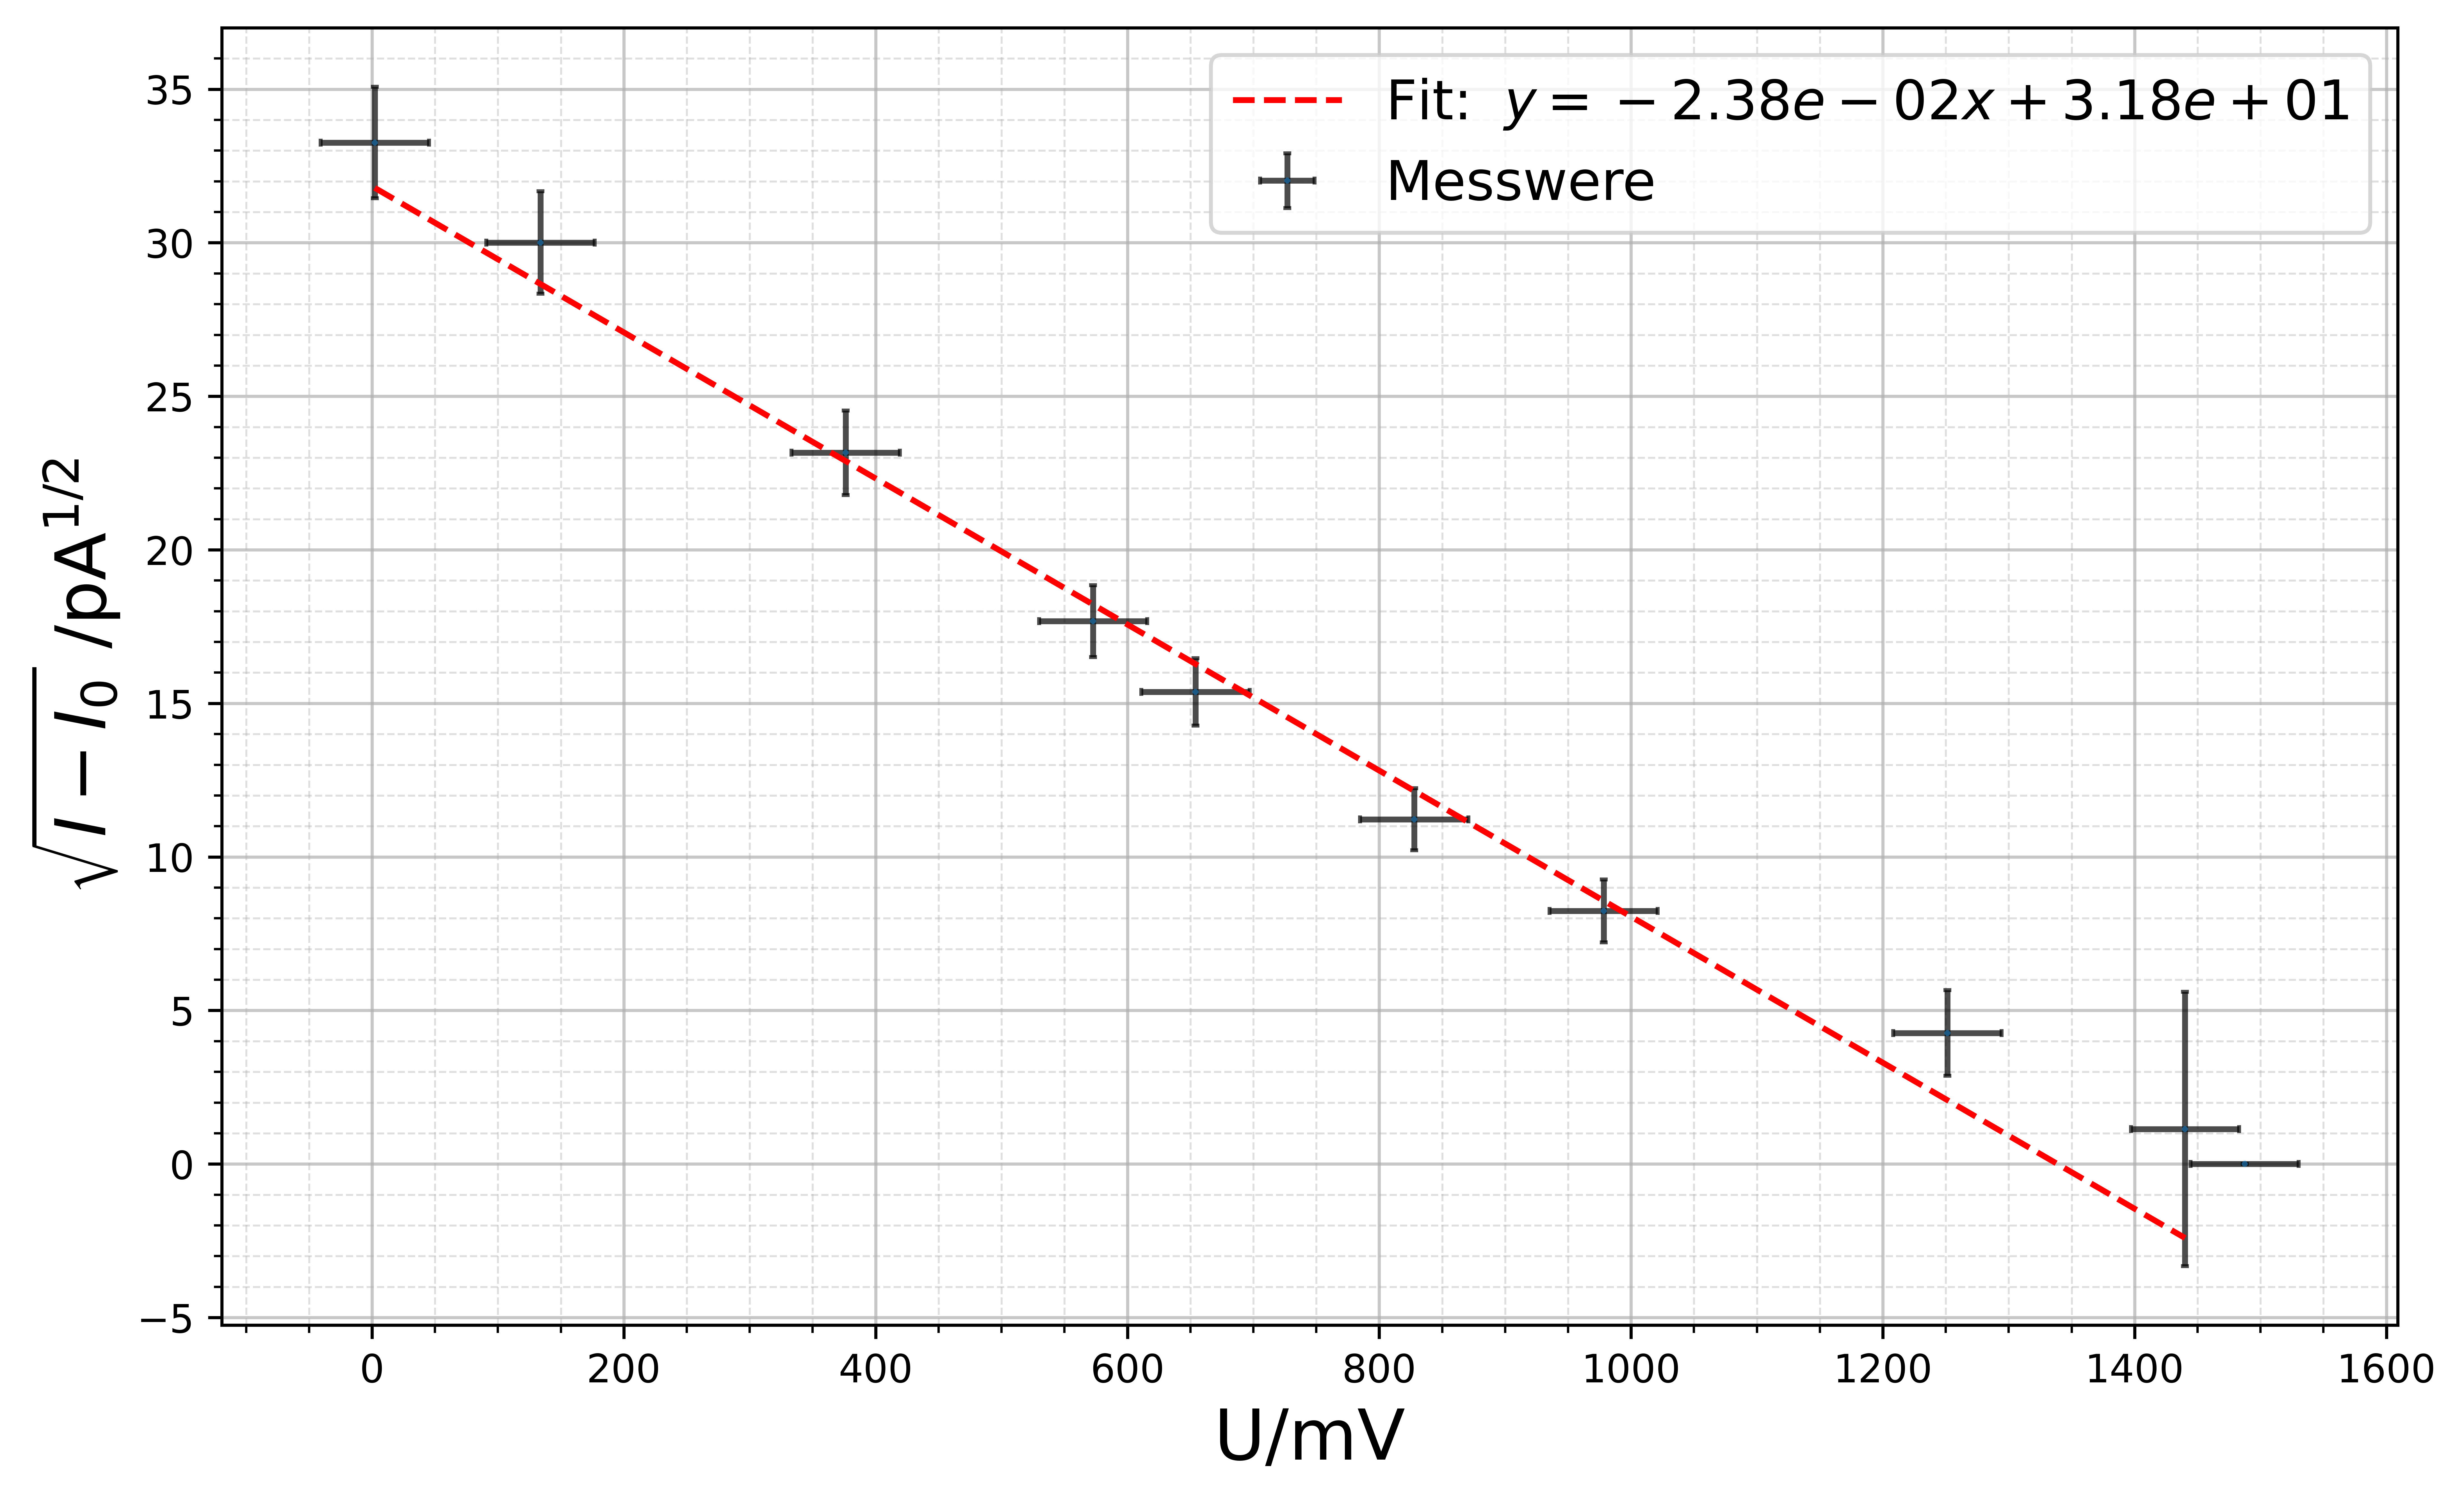
\includegraphics[width=0.95\linewidth]{figs/463_1.png}
    \captionof{figure}{%
      Messung 1 bei $\lambda=\SI{463}{\nm}$. 
      Die Werte und Unsicherheiten sind in \cref{tab:463_first}.%
    }
    \label{fig:463_first}
  \end{minipage}\hfill
  \begin{minipage}[t]{\linewidth}
    \centering
    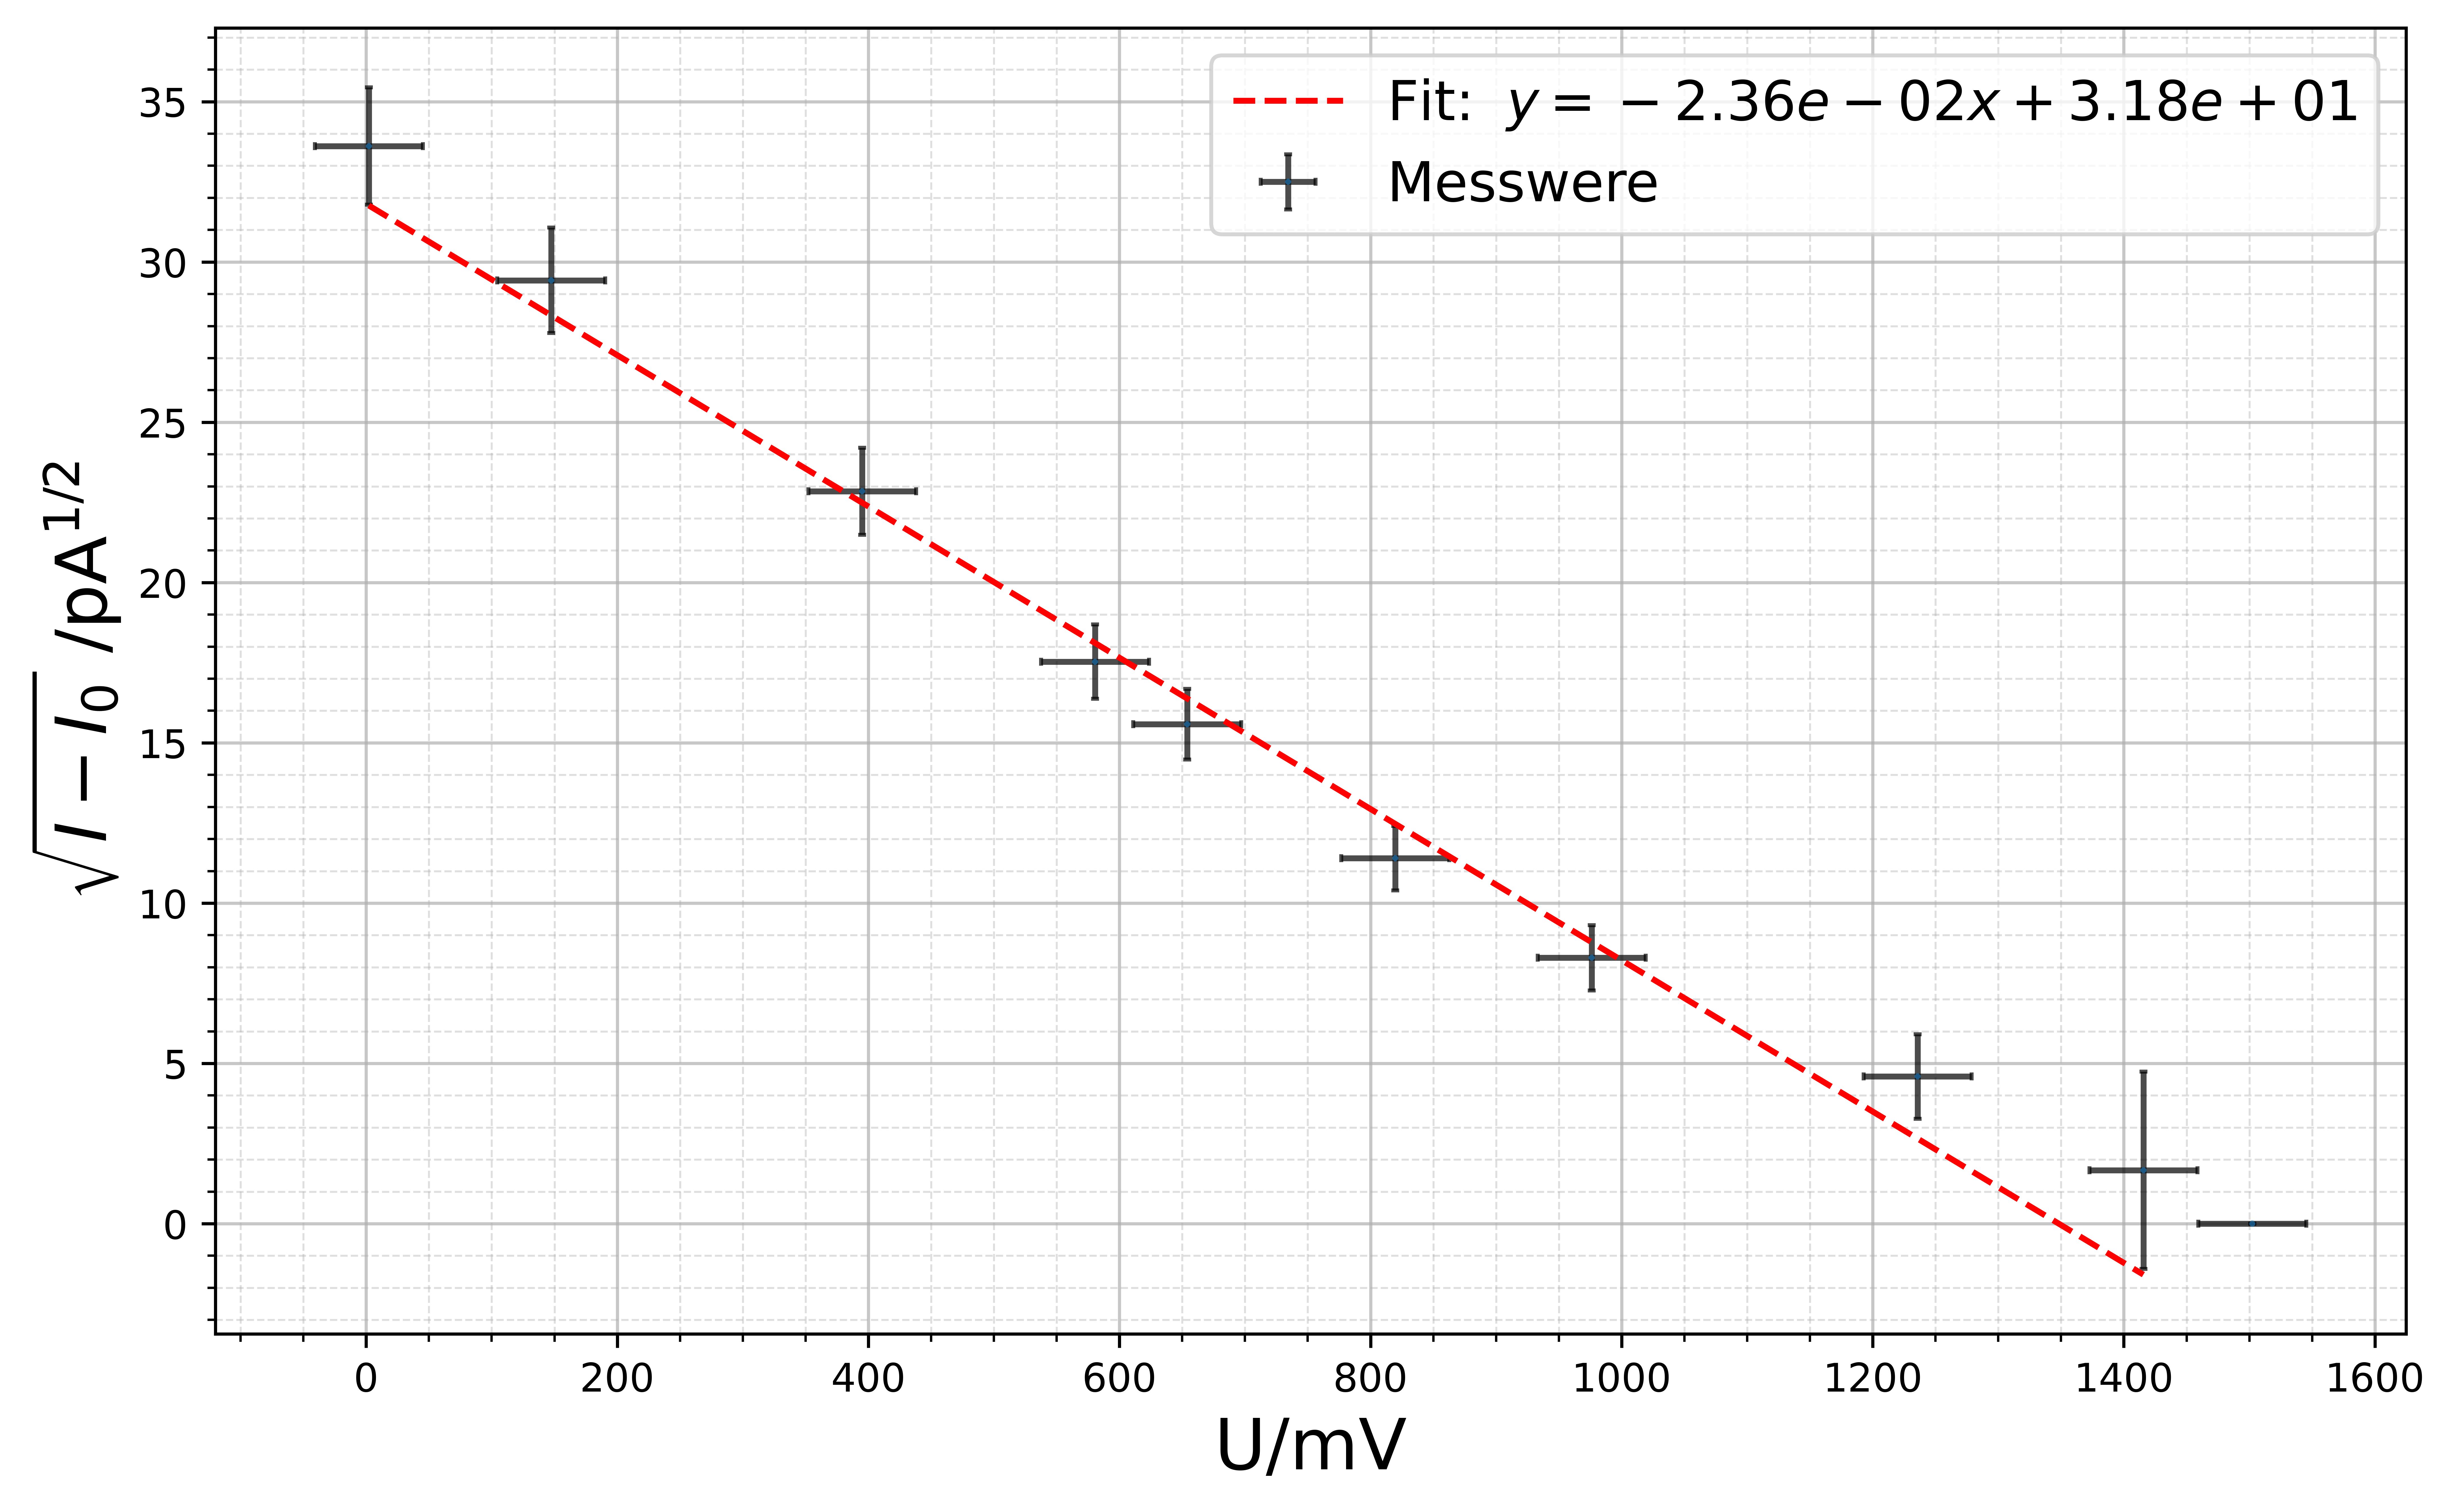
\includegraphics[width=0.95\linewidth]{figs/463_2.png}
    \captionof{figure}{%
      Messung 2 bei $\lambda=\SI{463}{\nm}$. 
      Die Werte und Unsicherheiten sind in \cref{tab:463_second}.%
    }
    \label{fig:463_second}
  \end{minipage}
\end{figure}


\begin{figure}[H]
  \centering
  \begin{minipage}[t]{\linewidth}
    \centering
    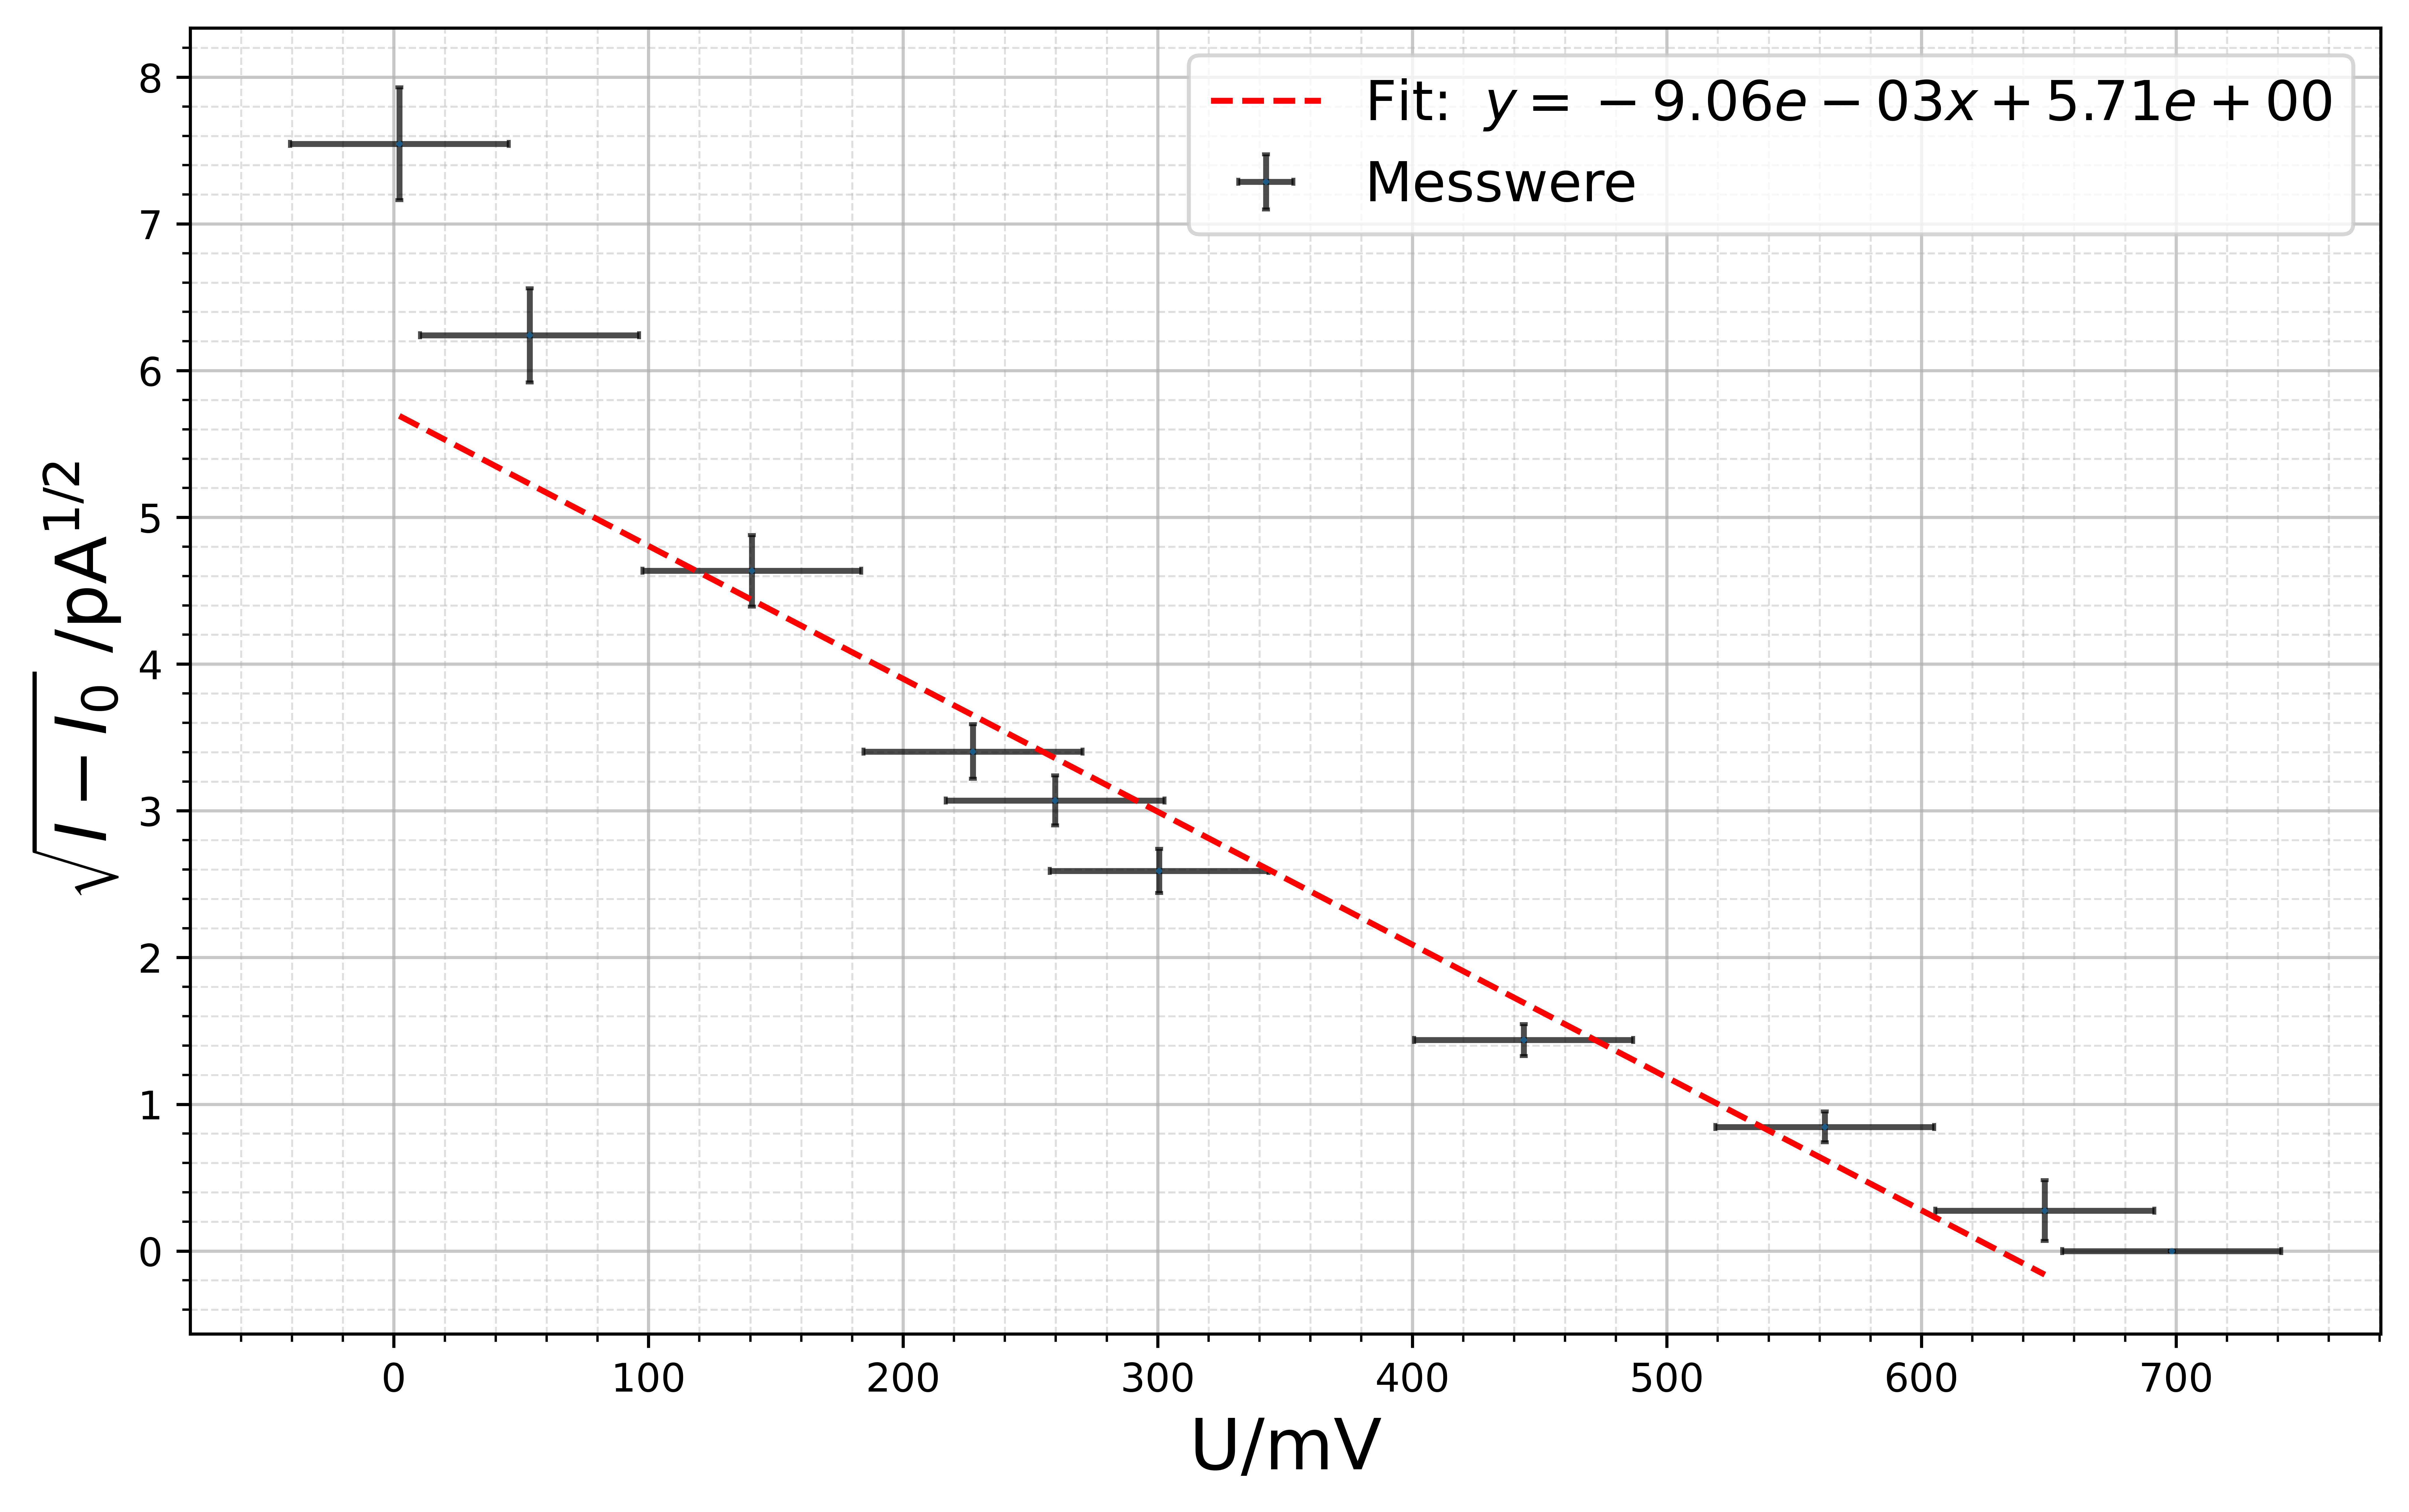
\includegraphics[width=0.95\linewidth]{figs/546_1.png}
    \captionof{figure}{%
      Messung 1 bei $\lambda=\SI{546}{\nm}$. 
      Die Werte und Unsicherheiten sind in \cref{tab:546_first}.%
    }
    \label{fig:546_first}
  \end{minipage}\hfill
  \begin{minipage}[t]{\linewidth}
    \centering
    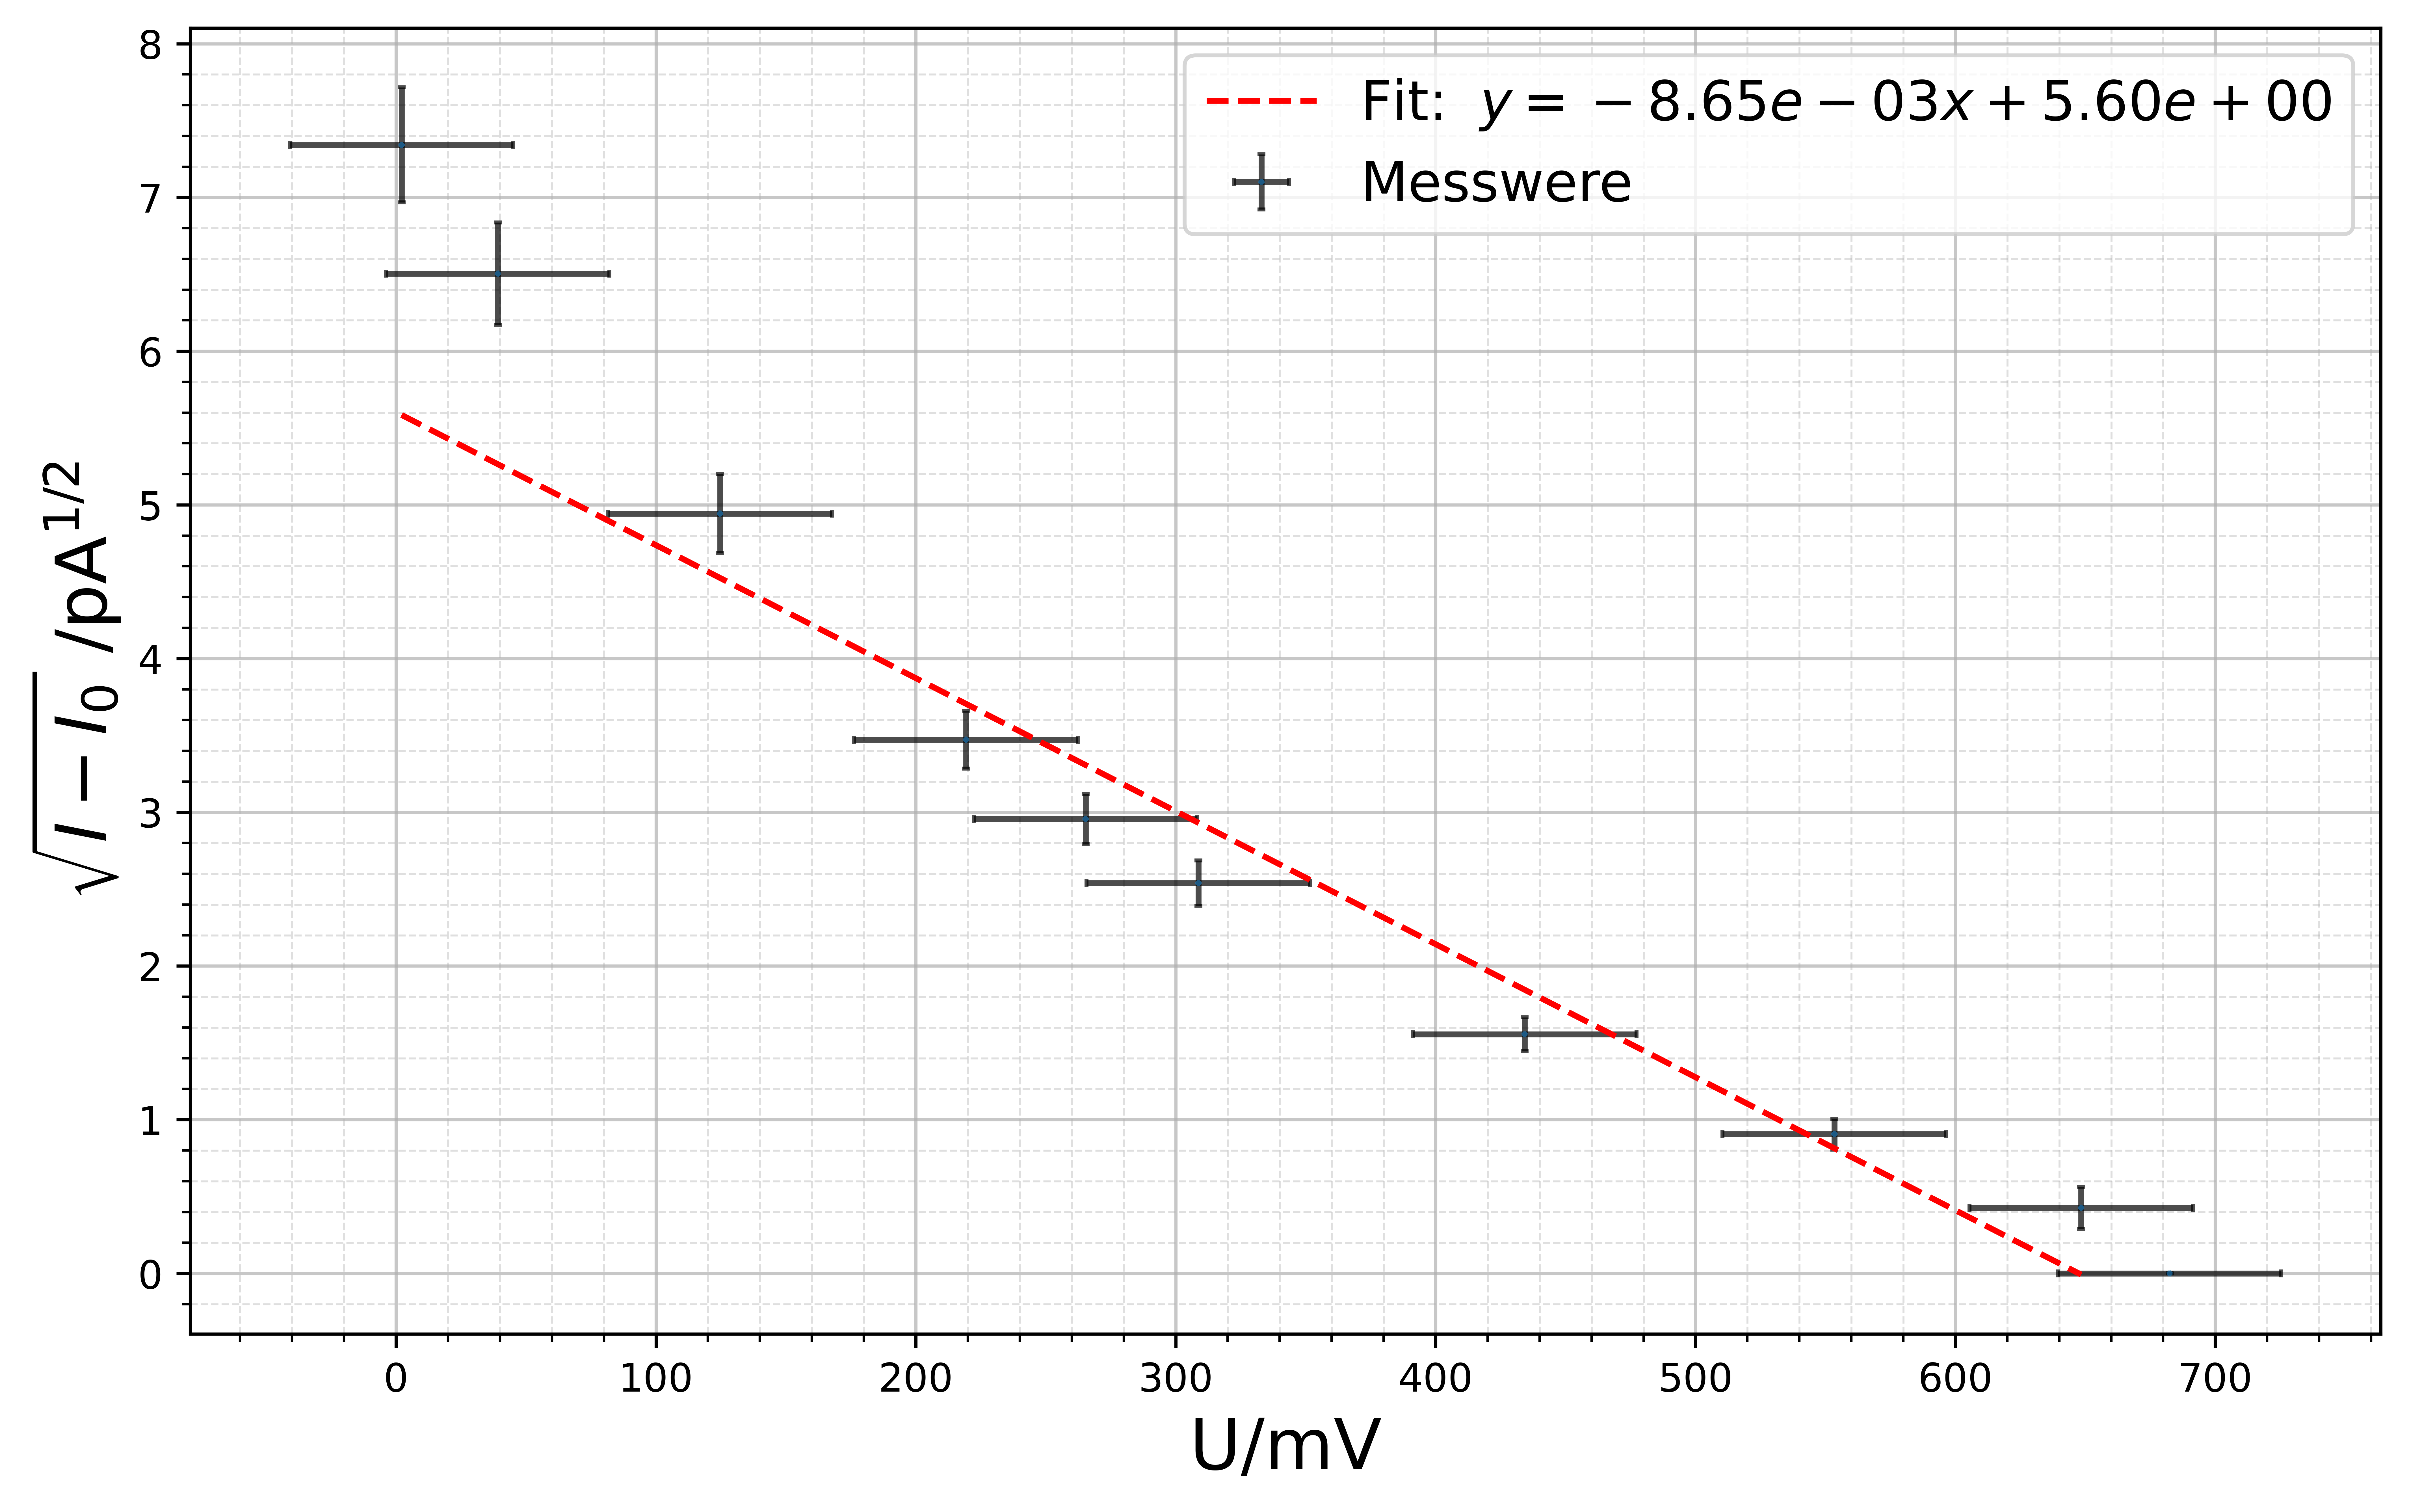
\includegraphics[width=0.95\linewidth]{figs/546_2.png}
    \captionof{figure}{%
      Messung 2 bei $\lambda=\SI{546}{\nm}$. 
      Die Werte und Unsicherheiten sind in \cref{tab:546_second}.%
    }
    \label{fig:546_second}
  \end{minipage}
\end{figure}

\begin{figure}[H]
  \centering
  \begin{minipage}[t]{\linewidth}
    \centering
    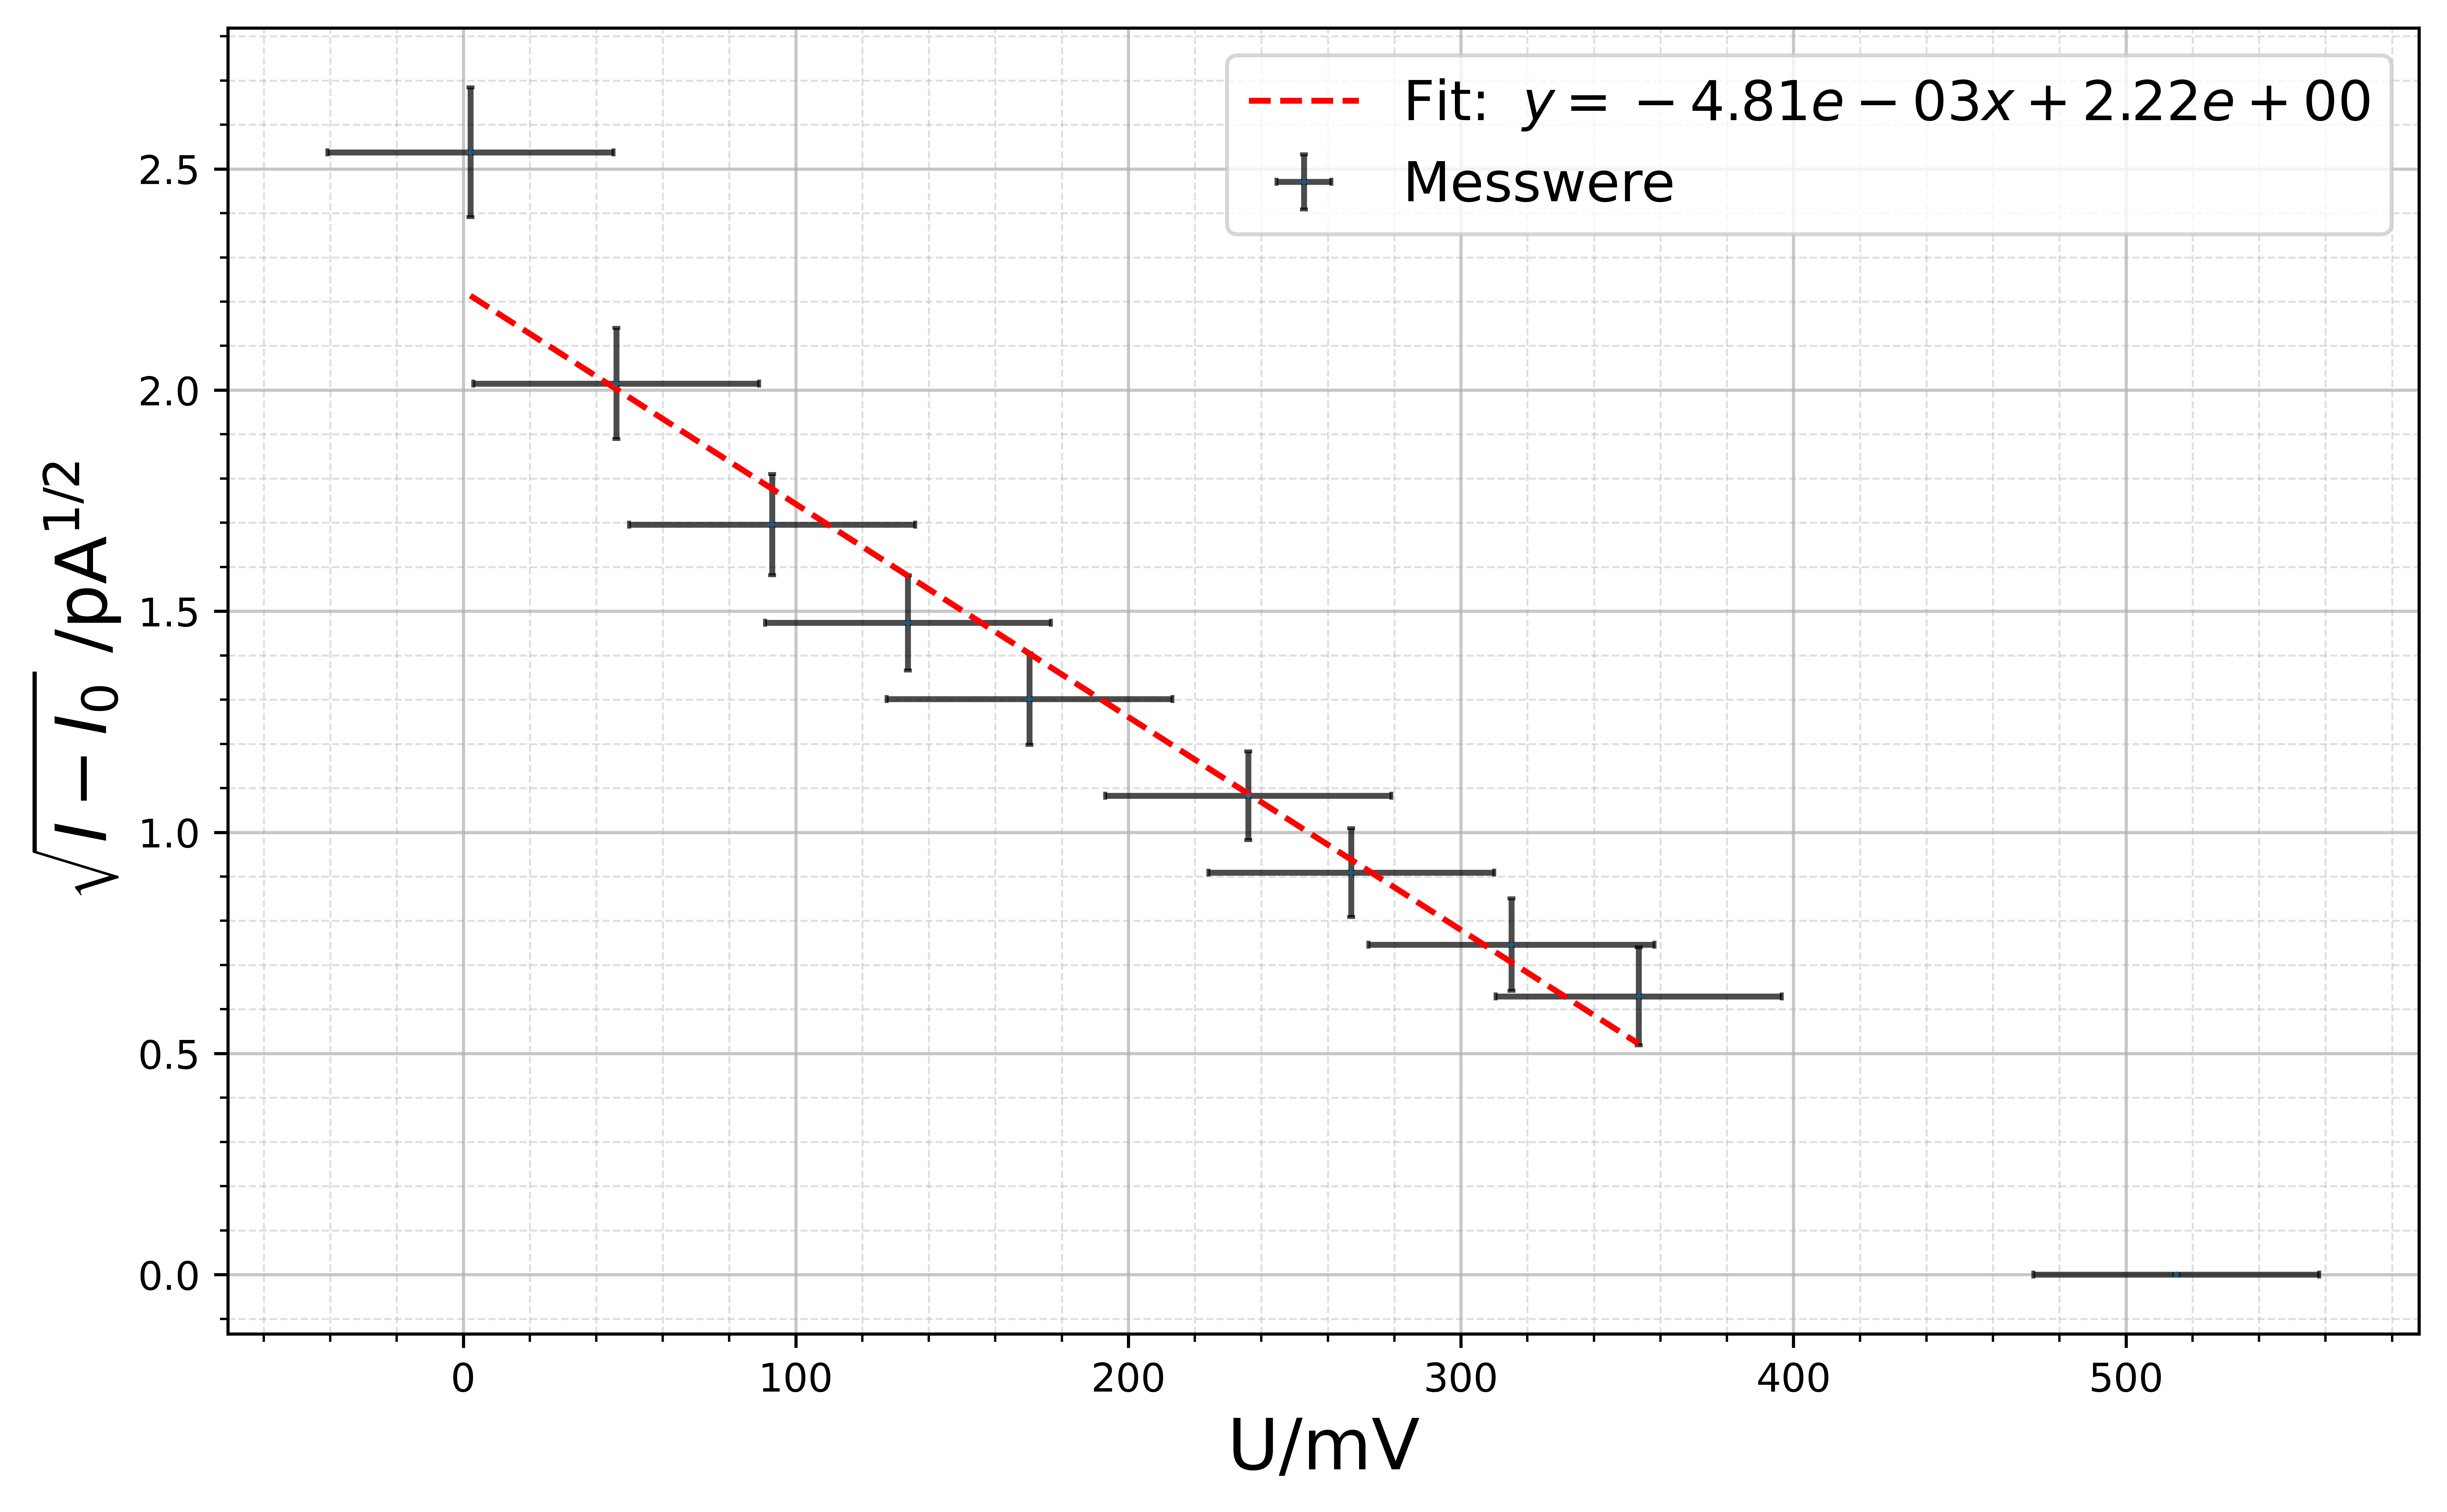
\includegraphics[width=0.95\linewidth]{figs/578_1.png}
    \captionof{figure}{%
      Messung 1 bei $\lambda=\SI{578}{\nm}$. 
      Die Werte und Unsicherheiten sind in \cref{tab:578_first}.%
    }
    \label{fig:578_first}
  \end{minipage}\hfill
  \begin{minipage}[t]{\linewidth}
    \centering
    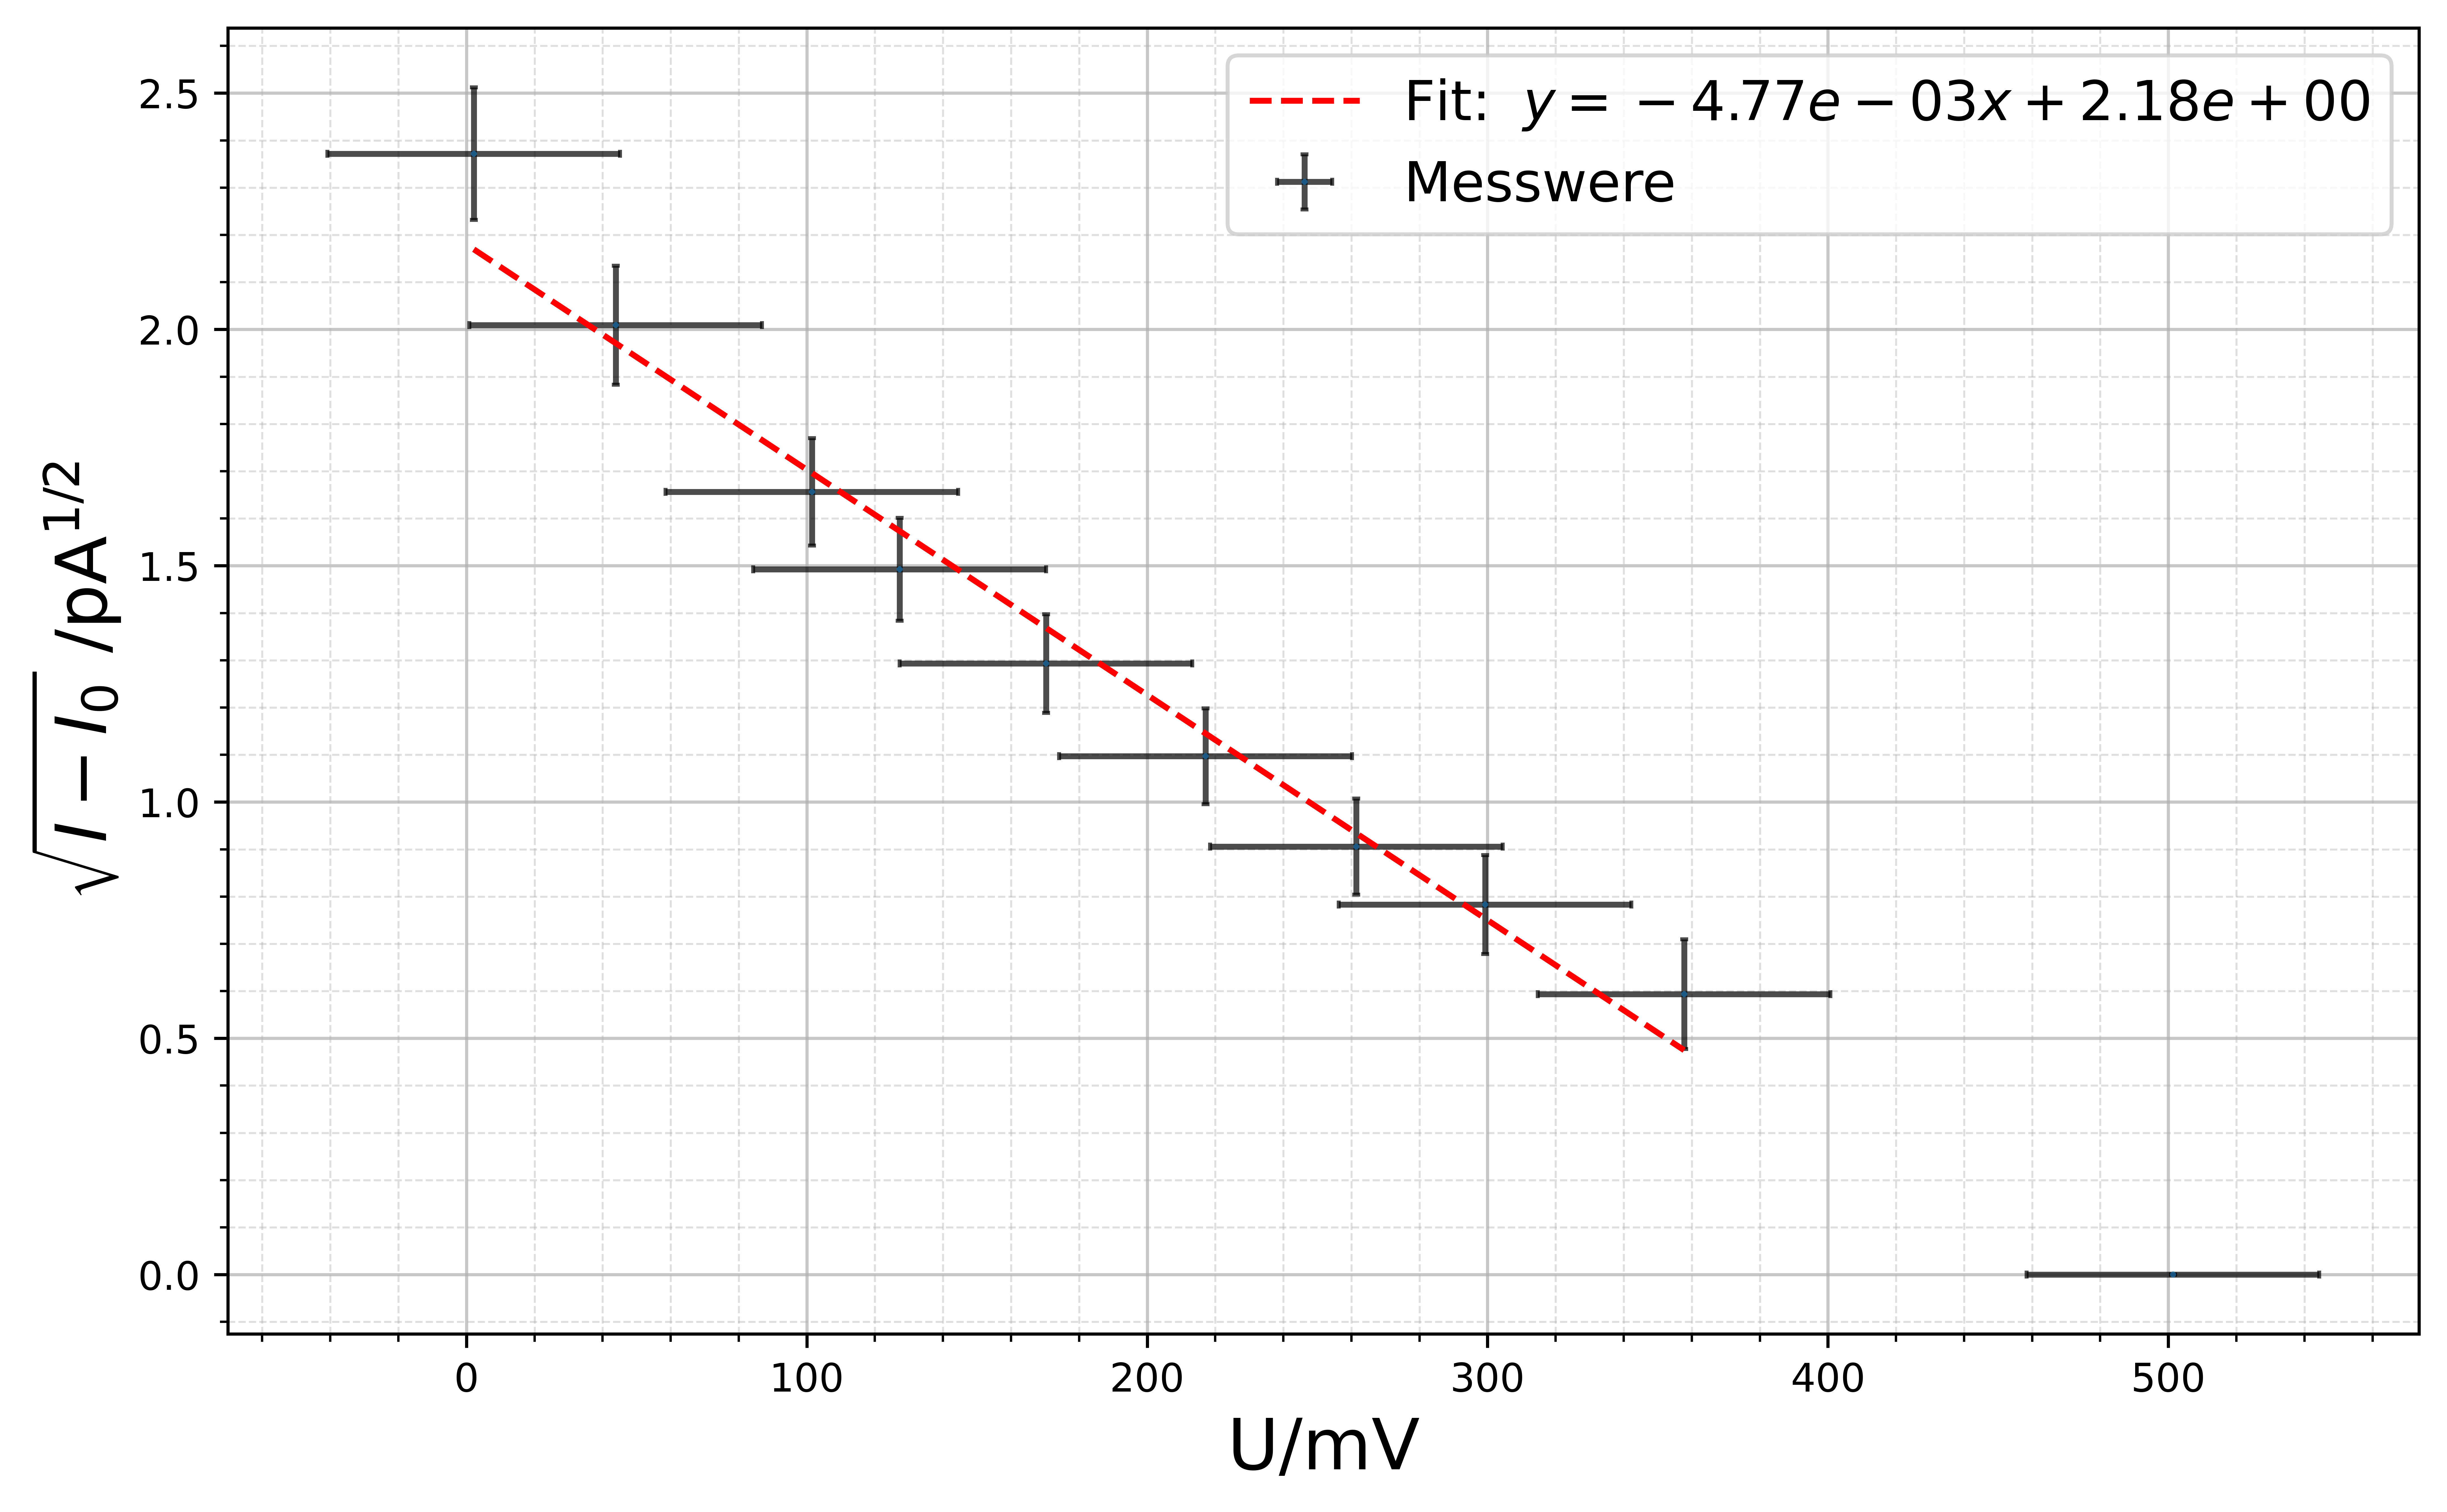
\includegraphics[width=0.95\linewidth]{figs/578_2.png}
    \captionof{figure}{%
      Messung 2 bei $\lambda=\SI{578}{\nm}$. 
      Die Werte und Unsicherheiten sind in \cref{tab:578_second}.%
    }
    \label{fig:578_second}
  \end{minipage}
\end{figure}

\subsection*{Balmer Serie}

\section{Tabellen}
\subsection*{Photoeffekt}
%=======================================================================================================================================================================================================
\begin{table}[H]
\centering
\resizebox{\columnwidth}{!}{
\begin{tabular}{|c|c|c|c|c|c|c|c|}
\hline
\multicolumn{4}{|c|}{$\lambda = \SI{365}{\nm}$}
  & \multicolumn{4}{c|}{$\lambda = \SI{405}{\nm}$} \\ \hline
\multicolumn{2}{|c|}{Messung 1} & \multicolumn{2}{c|}{Messung 2}
  & \multicolumn{2}{c|}{Messung 1} & \multicolumn{2}{c|}{Messung 2} \\ \hline
$U_G {[\si{mV}]}$   & $U_{ph} {[\si{mV}]}$  & $U_G {[\si{mV}]}$  & $U_{ph} {[\si{mV}]}$ & $U_G {[\si{mV}]}$    & $U_{ph} {[\si{mV}]}$ & $U_G {[\si{mV}]}$  & $U_{ph} {[\si{mV}]}$ \\ \hline
0,5             & 2380,0            & 0,5           & 2382,0           & 0,5             & 900,0            & 0,5           & 914,0            \\ \hline
30,5            & 2070,0            & 35,6          & 2065,0           & 41,5            & 722,0            & 36,0            & 740,0            \\ \hline
84,2            & 1630,0            & 84,6          & 1624,0           & 49,4            & 680,0            & 53,9          & 665,0            \\ \hline
121,0             & 1325,0            & 120,5         & 1334,0           & 105,4           & 450,0            & 102,0           & 464,0            \\ \hline
152,9           & 1071,0            & 156,3         & 1061,0           & 149,6           & 293,8          & 152,9         & 286,9,0          \\ \hline
160,7           & 1025,0            & 170,3         & 951,0            & 167,7           & 245,0            & 165,6         & 250,5          \\ \hline
182,4           & 883,0             & 180,8         & 892,0            & 174,5           & 226,9          & 178,2         & 215,6          \\ \hline
190,7           & 823,0             & 194,8         & 795,0            & 201,7           & 161,2          & 200,3         & 164,8          \\ \hline
217,9           & 655,0             & 219,4         & 653,0            & 213,7           & 139,5          & 217,5         & 230,0            \\ \hline
270,0             & 396,0             & 271,1         & 392,0            & 247,4           & 86,1           & 254,1         & 78,8           \\ \hline
287,0             & 333,3           & 287,4         & 325,0            & 267,7           & 63,5           & 273,2         & 58,2           \\ \hline
355,7           & 152,7           & 359,2         & 148,8          & 289,6           & 45,8           & 293,0           & 24,8           \\ \hline
396,3           & 79,9            & 397,2         & 95,6           & 301,9           & 38,8           & 304,7         & 36,5           \\ \hline
452,0             & 32,9            & 455,0           & 29,2           & 352,9           & 14,8           & 345,3         & 17,6           \\ \hline
472,0             & 14,1            & 477,0          & 11,7           & 378,1           & 5,1            & 384,8         & 3,2            \\ \hline
517,0             & 1,1             & 516,0           & 1,4            & 410,0             & 1,1            & 405,0           & 1,1            \\ \hline
\end{tabular}%
}
\caption{Messwerte der Photospannung $U_{ph}$ bei Gegenspannung $U_G$ für $\lambda$ = $\SI{365}{\nm}$ und $\lambda$ = $\SI{405}{\nm}$, wobei $\Delta U_{ph} = 0.1 \cdot U_{ph} + 10\,\si{\milli\volt}, \quad
 \Delta U_{G} = 10 \si{\milli\volt}$}
\label{tab:365and405}
\end{table}
%=======================================================================================================================================================================================================

\begin{table}[H]
\centering
\resizebox{0.5\columnwidth}{!}{%
  \begin{tabular}{|c|c|c|c|}
    \hline
    \multicolumn{4}{|c|}{$\lambda = \SI{463}{\nm}$} \\ \hline
    \multicolumn{2}{|c|}{Messung 1} & \multicolumn{2}{c|}{Messung 2} \\ \hline
    $U_G {[\si{mV}]}$ & $U_{ph} {[\si{mV}]}$ & $U_G {[\si{mV}]}$ & $U_{ph} {[\si{mV}]}$ \\ \hline
    0,5   & 1107,0   & 0,5   & 1130,0   \\ \hline
    31,1  & 901,0    & 34,3  & 866,0    \\ \hline
    87,5  & 537,0    & 91,9  & 522,0    \\ \hline
    133,2 & 313,1    & 135,0 & 307,4    \\ \hline
    152,1 & 236,9    & 152,1 & 242,8    \\ \hline
    192,5 & 126,6    & 190,6 & 130,0    \\ \hline
    227,5 & 68,5     & 227,0 & 68,8     \\ \hline
    291,0 & 18,8     & 287,4 & 21,1     \\ \hline
    334,9 & 1,9      & 329,2 & 2,8      \\ \hline
    345,9 & 0,6      & 349,4 & 0,0      \\ \hline
  \end{tabular}%
}
\caption{Messwerte der Photospannung $U_{ph}$ bei Gegenspannung $U_G$ für $\lambda = \SI{463}{\nm}$, mit $\Delta U_{ph} = 0.1 \cdot U_{ph} + \SI{10}{\milli\volt}$ und $\Delta U_{G} = \SI{10}{\milli\volt}$.}
\label{tab:463nm}
\end{table}
%=======================================================================================================================================================================================================
\begin{table}[H]
\centering
\resizebox{\columnwidth}{!}{%
  \begin{tabular}{|c|c|c|c|c|c|c|c|}
    \hline
    \multicolumn{4}{|c|}{$\lambda = \SI{546}{\nm}$}
      & \multicolumn{4}{c|}{$\lambda = \SI{578}{\nm}$} \\ \hline
    \multicolumn{2}{|c|}{Messung 1} & \multicolumn{2}{c|}{Messung 2}
      & \multicolumn{2}{c|}{Messung 1} & \multicolumn{2}{c|}{Messung 2} \\ \hline
    $U_G {[\si{mV}]}$ & $U_{ph} {[\si{mV}]}$ & $U_G {[\si{mV}]}$ & $U_{ph} {[\si{mV}]}$
      & $U_G {[\si{mV}]}$ & $U_{ph} {[\si{mV}]}$ & $U_G {[\si{mV}]}$ & $U_{ph} {[\si{mV}]}$ \\ \hline
    0,5   & 5700,0   & 0,5   & 5390,0
      & 0,5   & 644,0    & 0,5   & 565,0    \\ \hline
    32,7  & 2155,0   & 29,0  & 2444,0
      & 10,7  & 406,0    & 10,2  & 406,0    \\ \hline
    12,4  & 3900,0   & 9,1   & 4230,0
      & 21,6  & 287,5    & 23,6  & 276,8    \\ \hline
    52,9  & 1165,0   & 51,0  & 1206,0
      & 31,1  & 217,2    & 29,6  & 225,1    \\ \hline
    69,9  & 677,0    & 61,7  & 874,0
      & 39,6  & 169,3    & 39,6  & 169,6    \\ \hline
    60,4  & 949,0    & 71,8  & 645,0
      & 54,9  & 117,2    & 50,5  & 122,7    \\ \hline
    103,2 & 212,9    & 101,0 & 242,1
      & 62,1  & 82,6     & 60,8  & 84,4     \\ \hline
    130,7 & 77,7     & 128,7 & 82,2
      & 73,3  & 55,7     & 69,6  & 63,7     \\ \hline
    150,8 & 13,8     & 150,8 & 18,3
      & 82,2  & 39,6     & 83,2  & 37,6     \\ \hline
    162,4 & 6,2      & 158,7 & 0,1
      & 119,8 & 0,0      & 116,6 & 2,4      \\ \hline
  \end{tabular}%
}
\caption{Messwerte der Photospannung $U_{ph}$ bei Gegenspannung $U_G$ für $\lambda = \SI{546}{\nm}$ und $\lambda = \SI{578}{\nm}$, wobei $\Delta U_{ph} = 0.1 \cdot U_{ph} + \SI{10}{\milli\volt}$ und $\Delta U_{G} = \SI{10}{\milli\volt}$.}
\label{tab:546and578}
\end{table}
%=======================================================================================================================================================================================================
\begin{table}[H]
\centering
\resizebox{0.5\columnwidth}{!} \\ \hline
    $U_G {[\si{mV}]}$ & $U_{ph} {[\si{mV}]}$ & $U_G {[\si{mV}]}$ & $U_{ph} {[\si{mV}]}$ \\ \hline
    0,4    & 9200,0 & 0,5   & 4040,0 \\ \hline
    100,2  & 5760,0 & 106,6 & 2417,0 \\ \hline
    200,8  & 2939,0 & 203,3 & 1296,0 \\ \hline
    259,3  & 1806,0 & 235,6 &  974,0 \\ \hline
    299,3  & 1172,0 & 255,8 &  806,0 \\ \hline
    330,4  &  823,0 & 279,8 &  630,0 \\ \hline
    364,5  &  549,0 & 303,6 &  491,0 \\ \hline
    402,0  &  337,6 & 350,8 &  282,4 \\ \hline
    453,0  &  111,6 & 404,0 &  147,8 \\ \hline
    504,0  &   12,2 & 450,0 &   58,8 \\ \hline
    1020,0 &    1,5 & 510,0 &   10,0 \\ \hline
  \end{tabular}%
}
\caption{Messwerte der Photospannung $U_{ph}$ bei Gegenspannung $U_G$ für $\lambda = \SI{365}{\nm}$ (Maximalwerte und 50\%-Punkt), wobei $\Delta U_{ph} = 0.1 \cdot U_{ph} + \SI{10}{\milli\volt}$ und $\Delta U_{G} = \SI{10}{\milli\volt}$.}
\label{tab:365_max_50}
\end{table}
%=======================================================================================================================================================================================================
\begin{table}[H]
\centering
\resizebox{0.75\columnwidth}{!}{%
\begin{tabular}{|c|c|c|c|c|c|}
\hline
$U$ [\si{\milli\volt}] & $\Delta U$ [\si{\milli\volt}] 
  & $I$ [\si{\pico\ampere}] & $\Delta I$ [\si{\pico\ampere}] 
  & $\sqrt{I - I_0}$ [\si{\sqrt{\pico\ampere}}] 
  & $\Delta\sqrt{I - I_0}$ [\si{\sqrt{\pico\ampere}}] \\ \hline
   2.15 &  43.00 & 2380.00 & 248.00 &  48.77 & 2.54 \\ \hline
 131.15 &  43.00 & 2070.00 & 217.00 &  45.49 & 2.39 \\ \hline
 362.06 &  43.00 & 1630.00 & 173.00 &  40.36 & 2.14 \\ \hline
 520.30 &  43.00 & 1325.00 & 142.50 & 36.39 & 1.96 \\ \hline
 657.47 &  43.00 & 1071.00 & 117.10 & 32.71 & 1.79 \\ \hline
 691.01 &  43.00 & 1025.00 & 112.50 & 32.00 & 1.76 \\ \hline
 784.32 &  43.00 &  883.00 &  98.30 & 29.70 & 1.66 \\ \hline
 820.01 &  43.00 &  823.00 &  92.30 & 28.67 & 1.61 \\ \hline
 936.97 &  43.00 &  655.00 &  75.50 & 25.57 & 1.48 \\ \hline
1161.00 &  43.00 &  396.00 &  49.60 & 19.87 & 1.25 \\ \hline
1234.10 &  43.00 &  333.30 &  43.33 & 18.23 & 1.19 \\ \hline
1529.51 &  43.00 &  152.70 &  25.27 & 12.31 & 1.03 \\ \hline
1704.09 &  43.00 &   79.90 &  17.99 &  8.88 & 1.01 \\ \hline
1943.60 &  43.00 &   32.90 &  13.29 &  5.64 & 1.18 \\ \hline
2029.60 &  43.00 &   14.10 &  11.41 &  3.61 & 1.58 \\ \hline
2223.10 &  43.00 &    1.10 &  10.11 &  0.00 & 0.00 \\ \hline
\end{tabular}%
}
\caption{Gemessenen Werte für die erste Messung bei $\lambda=\SI{365}{\nano\metre}$.  
Die Sättigungsspannung liegt bei $U_G= \SI{517.00}{\milli\volt}$, daraus folgt  
$I_0 = \SI{1.10 \pm 10.11}{\pico\ampere}$.}
\label{tab:365_first}
\end{table}

\begin{table}[H]
\centering
\resizebox{0.75\columnwidth}{!}{%
\begin{tabular}{|c|c|}
\hline
\textbf{Parameter} & \textbf{Wert} \\ \hline
Steigung $m$ [\si{\sqrt{\pico\ampere}/\milli\volt}]
  & $\num{-2.22e-2} \pm \num{5.58e-4}$ \\ \hline
Achsenabschnitt $b$ [\si{\sqrt{\pico\ampere}}]
  & $\num{4.70e1} \pm \num{7.48e-1}$ \\ \hline
$\mathrm{\chi}^2$
  & $\num{8.28}$ \\ \hline
Freiheitsgrade (dof)
  & 13 \\ \hline
$\mathrm{\chi}^2 / \mathrm{dof}$
  & $\num{0.637}$ \\ \hline
Abbrems­spannung $U_0$ [\si{\milli\volt}]
  & $\num{2117.12 \pm 62.98}$ \\ \hline
\end{tabular}%
}
\caption{Ergebnisse des gewichteten linearen $\mathrm{\chi}^2$-Fits zur Bestimmung der Abbrems­spannung für die erste Messung bei $\lambda=\SI{365}{\nano\metre}$. Die hier gezeigten Werte stammen aus Tabelle \ref{tab:365_first}.}
\label{tab:365_first_chi2}
\end{table}

%=======================================================================================================================================================================================================

\begin{table}[H]
\centering
\resizebox{0.75\columnwidth}{!}{%
\begin{tabular}{|c|c|c|c|c|c|}
\hline
$U$ [\si{\milli\volt}] & $\Delta U$ [\si{\milli\volt}] 
  & $I$ [\si{\pico\ampere}] & $\Delta I$ [\si{\pico\ampere}] 
  & $\sqrt{I - I_0}$ [\si{\sqrt{\pico\ampere}}] 
  & $\Delta\sqrt{I - I_0}$ [\si{\sqrt{\pico\ampere}}] \\ \hline
   2.15 &  43.00 & 2382.00 & 248.20 &  48.79 &  2.54 \\ \hline
 153.08 &  43.00 & 2065.00 & 216.50 &  45.43 &  2.38 \\ \hline
 363.78 &  43.00 & 1624.00 & 172.40 &  40.28 &  2.14 \\ \hline
 518.15 &  43.00 & 1334.00 & 143.40 &  36.50 &  1.96 \\ \hline
 672.09 &  43.00 & 1061.00 & 116.10 &  32.55 &  1.78 \\ \hline
 732.29 &  43.00 &  951.00 & 105.10 &  30.82 &  1.71 \\ \hline
 777.44 &  43.00 &  892.00 &  99.20 &  29.84 &  1.66 \\ \hline
 837.64 &  43.00 &  795.00 &  89.50 &  28.17 &  1.59 \\ \hline
 943.42 &  43.00 &  653.00 &  75.30 &  25.53 &  1.47 \\ \hline
1165.73 &  43.00 &  392.00 &  49.20 &  19.76 &  1.24 \\ \hline
1235.82 &  43.00 &  325.00 &  42.50 &  17.99 &  1.18 \\ \hline
1544.56 &  43.00 &  148.80 &  24.88 &  12.14 &  1.02 \\ \hline
1707.96 &  43.00 &   95.60 &  19.56 &   9.71 &  1.01 \\ \hline
1956.50 &  43.00 &   29.20 &  12.92 &   5.27 &  1.23 \\ \hline
2051.10 &  43.00 &   11.70 &  11.17 &   3.21 &  1.74 \\ \hline
2218.80 &  43.00 &    1.40 &  10.14 &   0.00 &  0.00 \\ \hline
\end{tabular}%
}
\caption{Gemessenen Werte für die zweite Messung bei $\lambda=\SI{365}{\nano\metre}$.  
Die Sättigungsspannung liegt bei $U_G=\SI{516.00}{\milli\volt}$, daraus folgt  
$I_0 = \SI[separate-uncertainty=true]{1.40 \pm 10.14}{\pico\ampere}$.}
\label{tab:365_second}
\end{table}

\begin{table}[H]
\centering
\resizebox{0.75\columnwidth}{!}{%
\begin{tabular}{|c|c|}
\hline
\textbf{Parameter} & \textbf{Wert} \\ \hline
Steigung $m$ [\si{\sqrt{\pico\ampere}/\milli\volt}] 
  & $\num{-2.20e-2} \pm \num{5.73e-4}$ \\ \hline
Achsenabschnitt $b$ [\si{\sqrt{\pico\ampere}}] 
  & $\num{4.69e1} \pm \num{7.63e-1}$ \\ \hline
$\mathrm{\chi}^2$ 
  & $\num{8.45}$ \\ \hline
Freiheitsgrade (dof) 
  & 13 \\ \hline
$\mathrm{\chi}^2 / \mathrm{dof}$ 
  & $\num{0.650}$ \\ \hline
Abbrems­spannung $U_0$ [\si{\milli\volt}] 
  & $\num{2131.82 \pm 65.47}$ \\ \hline
\end{tabular}%
}
\caption{Ergebnisse des gewichteten linearen $\mathrm{\chi}^2$-Fits zur Bestimmung der Abbrems­spannung für die zweite Messung bei $\lambda=\SI{365}{\nano\metre}$. Die hier gezeigten Werte stammen aus Tabelle \ref{tab:365_second}.}
\label{tab:365_second_chi2}
\end{table}


%=======================================================================================================================================================================================================
\begin{table}[H]
\centering
\resizebox{0.75\columnwidth}{!}{%
\begin{tabular}{|c|c|c|c|c|c|}
\hline
$U$ [\si{\milli\volt}] & $\Delta U$ [\si{\milli\volt}] 
  & $I$ [\si{\pico\ampere}] & $\Delta I$ [\si{\pico\ampere}] 
  & $\sqrt{I - I_0}$ [\si{\sqrt{\pico\ampere}}] 
  & $\Delta\sqrt{I - I_0}$ [\si{\sqrt{\pico\ampere}}] \\ \hline
   2.15 &  43.00 & 4040.00 & 414.00 &  63.48 & 3.26 \\ \hline
 458.38 &  43.00 & 2417.00 & 251.70 &  49.06 & 2.57 \\ \hline
 874.19 &  43.00 & 1296.00 & 139.60 &  35.86 & 1.95 \\ \hline
1013.08 &  43.00 &  974.00 & 107.40 &  31.05 & 1.73 \\ \hline
1099.94 &  43.00 &  806.00 &  90.60 &  28.21 & 1.61 \\ \hline
1203.14 &  43.00 &  630.00 &  73.00 &  24.90 & 1.47 \\ \hline
1305.48 &  43.00 &  491.00 &  59.10 &  21.93 & 1.35 \\ \hline
1508.44 &  43.00 &  282.40 &  38.24 &  16.50 & 1.16 \\ \hline
1737.20 &  43.00 &  147.80 &  24.78 &  11.74 & 1.06 \\ \hline
1935.00 &  43.00 &   58.80 &  15.88 &   6.99 & 1.14 \\ \hline
2193.00 &  43.00 &   10.00 &  11.00 &   0.00 & 0.00 \\ \hline
\end{tabular}%
}
\caption{Gemessenen Werte für die Messung bei 50 \% Intensität und $\lambda=\SI{365}{\nano\metre}$.  
Die Sättigungsspannung liegt bei $U_G=\SI{510.00}{\milli\volt}$, daraus folgt  
$I_0 = \SI[separate-uncertainty=true]{10.00 \pm 11.00}{\pico\ampere}$.}
\label{tab:365_50pct}
\end{table}

\begin{table}[H]
\centering
\resizebox{0.75\columnwidth}{!}{%
\begin{tabular}{|c|c|}
\hline
\textbf{Parameter} & \textbf{Wert} \\ \hline
Steigung $m$ [\si{\sqrt{\pico\ampere}/\milli\volt}] 
  & $\num{-2.79e-2} \pm \num{9.92e-4}$ \\ \hline
Achsenabschnitt $b$ [\si{\sqrt{\pico\ampere}}] 
  & $\num{5.96e1} \pm \num{1.45e0}$ \\ \hline
$\mathrm{\chi}^2$ 
  & $\num{6.55}$ \\ \hline
Freiheitsgrade (dof) 
  & 8 \\ \hline
$\mathrm{\chi}^2 / \mathrm{dof}$ 
  & $\num{0.819}$ \\ \hline
Abbrems­spannung $U_0$ [\si{\milli\volt}] 
  & $\num{2136.20 \pm 92.03}$ \\ \hline
\end{tabular}%
}
\caption{Ergebnisse des gewichteten linearen $\mathrm{\chi}^2$-Fits zur Bestimmung der Abbrems­spannung für die Messung bei $\lambda=\SI{365}{\nano\metre}$ mit 50\% Intensität. Die hier gezeigten Werte stammen aus Tabelle \ref{tab:365_50pct}.}
\label{tab:365_50_chi2}
\end{table}

%=======================================================================================================================================================================================================
\begin{table}[H]
\centering
\resizebox{0.75\columnwidth}{!}{%
\begin{tabular}{|c|c|c|c|c|c|}
\hline
$U$ [\si{\milli\volt}] & $\Delta U$ [\si{\milli\volt}] 
  & $I$ [\si{\pico\ampere}] & $\Delta I$ [\si{\pico\ampere}] 
  & $\sqrt{I - I_0}$ [\si{\sqrt{\pico\ampere}}] 
  & $\Delta\sqrt{I - I_0}$ [\si{\sqrt{\pico\ampere}}] \\ \hline
   1.72 &  43.00 & 9200.00 &  930.00 &  95.91 & 4.85 \\ \hline
 430.86 &  43.00 & 5760.00 &  586.00 &  75.88 & 3.86 \\ \hline
 863.44 &  43.00 & 2939.00 &  303.90 &  54.20 & 2.80 \\ \hline
1114.99 &  43.00 & 1806.00 &  190.60 &  42.48 & 2.24 \\ \hline
1286.99 &  43.00 & 1172.00 &  127.20 &  34.21 & 1.86 \\ \hline
1420.72 &  43.00 &  823.00 &   92.30 &  28.66 & 1.61 \\ \hline
1567.35 &  43.00 &  549.00 &   64.90 &  23.40 & 1.39 \\ \hline
1728.60 &  43.00 &  337.60 &   43.76 &  18.33 & 1.19 \\ \hline
1947.90 &  43.00 &  111.60 &   21.16 &  10.49 & 1.01 \\ \hline
2167.20 &  43.00 &   12.20 &   11.22 &   3.27 & 1.72 \\ \hline
4386.00 &  43.00 &    1.50 &   10.15 &   0.00 & 0.00 \\ \hline
\end{tabular}%
}
\caption{Gemessenen Werte für die Messung bei maximaler Intensität und $\lambda=\SI{365}{\nano\metre}$.  
Die Sättigungsspannung liegt bei $U_G=\SI{1020.00}{\milli\volt}$, daraus folgt  
$I_0 = \SI[separate-uncertainty=true]{1.50 \pm 10.15}{\pico\ampere}$.}
\label{tab:365_max}
\end{table}

\begin{table}[H]
\centering
\resizebox{0.75\columnwidth}{!}{%
\begin{tabular}{|c|c|}
\hline
\textbf{Parameter} & \textbf{Wert} \\ \hline
Steigung $m$ [\si{\sqrt{\pico\ampere}/\milli\volt}] 
  & $\num{-4.00e-2} \pm \num{1.57e-3}$ \\ \hline
Achsenabschnitt $b$ [\si{\sqrt{\pico\ampere}}] 
  & $\num{8.76e1} \pm \num{2.64e0}$ \\ \hline
$\mathrm{\chi}^2$ 
  & $\num{11.74}$ \\ \hline
Freiheitsgrade (dof) 
  & 8 \\ \hline
$\mathrm{\chi}^2 / \mathrm{dof}$ 
  & $\num{1.467}$ \\ \hline
Abbrems­spannung $U_0$ [\si{\milli\volt}] 
  & $\num{2190.00 \pm 108.37}$ \\ \hline
\end{tabular}%
}
\caption{Ergebnisse des gewichteten linearen $\mathrm{\chi}^2$-Fits zur Bestimmung der Abbrems­spannung für die Messung bei $\lambda=\SI{365}{\nano\metre}$ mit maximaler Intensität. Die hier gezeigten Werte stammen aus Tabelle \ref{tab:365_max}.}
\label{tab:365_max_chi2}
\end{table}

%=======================================================================================================================================================================================================
\begin{table}[H]
\centering
\resizebox{0.75\columnwidth}{!}{%
\begin{tabular}{|c|c|c|c|c|c|}
\hline
$U$ [\si{\milli\volt}] & $\Delta U$ [\si{\milli\volt}] 
  & $I$ [\si{\pico\ampere}] & $\Delta I$ [\si{\pico\ampere}] 
  & $\sqrt{I - I_0}$ [\si{\sqrt{\pico\ampere}}] 
  & $\Delta\sqrt{I - I_0}$ [\si{\sqrt{\pico\ampere}}] \\ \hline
   2.15 &  43.00 &  900.00 & 100.00 &  29.98 & 1.67 \\ \hline
 178.45 &  43.00 &  722.00 &  82.20 &  26.85 & 1.53 \\ \hline
 212.42 &  43.00 &  680.00 &  78.00 &  26.06 & 1.50 \\ \hline
 453.22 &  43.00 &  450.00 &  55.00 &  21.19 & 1.30 \\ \hline
 643.28 &  43.00 &  293.80 &  39.38 &  17.11 & 1.15 \\ \hline
 721.11 &  43.00 &  245.00 &  34.50 &  15.62 & 1.10 \\ \hline
 750.35 &  43.00 &  226.90 &  32.69 &  15.03 & 1.09 \\ \hline
 867.31 &  43.00 &  161.20 &  26.12 &  12.65 & 1.03 \\ \hline
 918.91 &  43.00 &  139.50 &  23.95 &  11.76 & 1.02 \\ \hline
1063.82 &  43.00 &   86.10 &  18.61 &   9.22 & 1.01 \\ \hline
1151.11 &  43.00 &   63.50 &  16.35 &   7.90 & 1.03 \\ \hline
1245.28 &  43.00 &   45.80 &  14.58 &   6.69 & 1.09 \\ \hline
1298.17 &  43.00 &   38.80 &  13.88 &   6.14 & 1.13 \\ \hline
1517.47 &  43.00 &   14.80 &  11.48 &   3.70 & 1.55 \\ \hline
1625.83 &  43.00 &    5.10 &  10.51 &   2.00 & 2.63 \\ \hline
1763.00 &  43.00 &    1.10 &  10.11 &   0.00 & 0.00 \\ \hline
\end{tabular}%
}
\caption{Gemessenen Werte für die erste Messung bei $\lambda=\SI{405}{\nano\metre}$.  
Die Sättigungsspannung liegt bei $U_G=\SI{410.00}{\milli\volt}$, daraus folgt  
$I_0 = \SI[separate-uncertainty=true]{1.10 \pm 10.11}{\pico\ampere}$.}
\label{tab:405_first}
\end{table}

\begin{table}[H]
\centering
\resizebox{0.75\columnwidth}{!}{%
\begin{tabular}{|c|c|}
\hline
\textbf{Parameter} & \textbf{Wert} \\ \hline
Steigung $m$ [\si{\sqrt{\pico\ampere}/\milli\volt}] 
  & $\num{-1.81e-2} \pm \num{5.50e-4}$ \\ \hline
Achsenabschnitt $b$ [\si{\sqrt{\pico\ampere}}] 
  & $\num{2.90e1} \pm \num{5.21e-1}$ \\ \hline
$\mathrm{\chi}^2$ 
  & $\num{5.80}$ \\ \hline
Freiheitsgrade (dof) 
  & 13 \\ \hline
$\mathrm{\chi}^2 / \mathrm{dof}$ 
  & $\num{0.446}$ \\ \hline
Abbrems­spannung $U_0$ [\si{\milli\volt}] 
  & $\num{1602.21 \pm 56.56}$ \\ \hline
\end{tabular}%
}
\caption{Ergebnisse des gewichteten linearen $\mathrm{\chi}^2$-Fits zur Bestimmung der Abbrems­spannung für die erste Messung bei $\lambda=\SI{405}{\nano\metre}$. Die hier gezeigten Werte stammen aus Tabelle \ref{tab:405_first}.}
\label{tab:405_first_chi2}
\end{table}

%=======================================================================================================================================================================================================
\begin{table}[H]
\centering
\resizebox{0.75\columnwidth}{!}{%
  \begin{tabular}{|c|c|c|c|c|c|}
    \hline
    $U$ [\si{\milli\volt}] & $\Delta U$ [\si{\milli\volt}]
      & $I$ [\si{\pico\ampere}] & $\Delta I$ [\si{\pico\ampere}]
      & $\sqrt{I - I_0}$ [\si{\sqrt{\pico\ampere}}]
      & $\Delta\sqrt{I - I_0}$ [\si{\sqrt{\pico\ampere}}] \\ \hline
       2.15 &  43.00 &  914.00 & 101.40 &  30.21 & 1.68 \\ \hline
 154.80 &  43.00 &  740.00 &  84.00 &  27.18 & 1.55 \\ \hline
 231.77 &  43.00 &  665.00 &  76.50 &  25.77 & 1.48 \\ \hline
 438.60 &  43.00 &  464.00 &  56.40 &  21.52 & 1.31 \\ \hline
 657.47 &  43.00 &  286.90 &  38.69 &  16.91 & 1.14 \\ \hline
 712.08 &  43.00 &  250.50 &  35.05 &  15.79 & 1.11 \\ \hline
 766.26 &  43.00 &  215.60 &  31.56 &  14.65 & 1.08 \\ \hline
 861.29 &  43.00 &  164.80 &  26.48 &  12.79 & 1.03 \\ \hline
 935.25 &  43.00 &  230.00 &  33.00 &  15.13 & 1.09 \\ \hline
1092.63 &  43.00 &   78.80 &  17.88 &   8.81 & 1.01 \\ \hline
1174.76 &  43.00 &   58.20 &  15.82 &   7.56 & 1.05 \\ \hline
1259.90 &  43.00 &   24.80 &  12.48 &   4.87 & 1.28 \\ \hline
1310.21 &  43.00 &   36.50 &  13.65 &   5.95 & 1.15 \\ \hline
1484.79 &  43.00 &   17.60 &  11.76 &   4.06 & 1.45 \\ \hline
1654.64 &  43.00 &    3.20 &  10.32 &   1.45 & 3.56 \\ \hline
1741.50 &  43.00 &    1.10 &  10.11 &   0.00 & 0.00 \\ \hline
  \end{tabular}%
}
\caption{Gemessenen Werte für die zweite Messung bei 
  $\lambda=\SI{405}{\nano\metre}$.  
  Die Sättigungsspannung liegt bei $U_G=\SI{405.00}{\milli\volt}$, daraus folgt  
  $I_0 = \SI[separate-uncertainty=true]{1.10 \pm 10.11}{\pico\ampere}$.}
\label{tab:405_second}
\end{table}

\begin{table}[H]
\centering
\resizebox{0.75\columnwidth}{!}{%
\begin{tabular}{|c|c|}
\hline
\textbf{Parameter} & \textbf{Wert} \\ \hline
Steigung $m$ [\si{\sqrt{\pico\ampere}/\milli\volt}] 
  & $\num{-1.83e-2} \pm \num{8.30e-4}$ \\ \hline
Achsenabschnitt $b$ [\si{\sqrt{\pico\ampere}}] 
  & $\num{2.95e1} \pm \num{7.84e-1}$ \\ \hline
$\mathrm{\chi}^2$ 
  & $\num{12.92}$ \\ \hline
Freiheitsgrade (dof) 
  & 13 \\ \hline
$\mathrm{\chi}^2 / \mathrm{dof}$ 
  & $\num{0.994}$ \\ \hline
Abbrems­spannung $U_0$ [\si{\milli\volt}] 
  & $\num{1612.02 \pm 84.74}$ \\ \hline
\end{tabular}%
}
\caption{Ergebnisse des gewichteten linearen $\mathrm{\chi}^2$-Fits zur Bestimmung der Abbrems­spannung für die zweite Messung bei $\lambda=\SI{405}{\nano\metre}$. Die hier gezeigten Werte stammen aus Tabelle \ref{tab:405_second}.}
\label{tab:405_second_chi2}
\end{table}

%=======================================================================================================================================================================================================
\begin{table}[H]
\centering
\resizebox{0.75\columnwidth}{!}{%
\begin{tabular}{|c|c|c|c|c|c|}
\hline
$U$ [\si{\milli\volt}] & $\Delta U$ [\si{\milli\volt}] 
  & $I$ [\si{\pico\ampere}] & $\Delta I$ [\si{\pico\ampere}] 
  & $\sqrt{I - I_0}$ [\si{\sqrt{\pico\ampere}}] 
  & $\Delta\sqrt{I - I_0}$ [\si{\sqrt{\pico\ampere}}] \\ \hline
   2.15 &  43.00 & 1107.00 & 120.70 &  33.26 & 1.81 \\ \hline
 133.73 &  43.00 &  901.00 & 100.10 &  30.01 & 1.67 \\ \hline
 376.25 &  43.00 &  537.00 &  63.70 &  23.16 & 1.38 \\ \hline
 572.76 &  43.00 &  313.10 &  41.31 &  17.68 & 1.17 \\ \hline
 654.03 &  43.00 &  236.90 &  33.69 &  15.37 & 1.10 \\ \hline
 827.75 &  43.00 &  126.60 &  22.66 &  11.22 & 1.01 \\ \hline
 978.25 &  43.00 &   68.50 &  16.85 &   8.24 & 1.02 \\ \hline
1251.30 &  43.00 &   18.80 &  11.88 &   4.27 & 1.39 \\ \hline
1440.07 &  43.00 &    1.90 &  10.19 &   1.14 & 4.47 \\ \hline
1487.37 &  43.00 &    0.60 &  10.06 &   0.00 & 0.00 \\ \hline
\end{tabular}%
}
\caption{Gemessenen Werte für die erste Messung bei $\lambda=\SI{463}{\nano\metre}$.  
Die Sättigungsspannung liegt bei $U_G=\SI{1487.37}{\milli\volt}$, daraus folgt  
$I_0 = \SI[separate-uncertainty=true]{0.60 \pm 10.06}{\pico\ampere}$.}
\label{tab:463_first}
\end{table}


\begin{table}[H]
\centering
\resizebox{0.75\columnwidth}{!}{%
\begin{tabular}{|c|c|}
\hline
\textbf{Parameter} & \textbf{Wert} \\ \hline
Steigung $m$ [\si{\sqrt{\pico\ampere}/\milli\volt}] 
  & $\num{-2.38e-2} \pm \num{1.22e-3}$ \\ \hline
Achsenabschnitt $b$ [\si{\sqrt{\pico\ampere}}] 
  & $\num{3.18e1} \pm \num{9.47e-1}$ \\ \hline
$\mathrm{\chi}^2$ 
  & $\num{6.31}$ \\ \hline
Freiheitsgrade (dof) 
  & 7 \\ \hline
$\mathrm{\chi}^2 / \mathrm{dof}$ 
  & $\num{0.901}$ \\ \hline
Abbrems­spannung $U_0$ [\si{\milli\volt}] 
  & $\num{1336.13 \pm 79.21}$ \\ \hline
\end{tabular}%
}
\caption{Ergebnisse des gewichteten linearen $\mathrm{\chi}^2$-Fits zur Bestimmung der Abbrems­spannung für die erste Messung bei $\lambda=\SI{463}{\nano\metre}$. Die hier gezeigten Werte stammen aus Tabelle \ref{tab:463_first}.}
\label{tab:463_first_chi2}
\end{table}

%=======================================================================================================================================================================================================
\begin{table}[H]
\centering
\resizebox{0.75\columnwidth}{!}{%
\begin{tabular}{|c|c|c|c|c|c|}
\hline
$U$ [\si{\milli\volt}] & $\Delta U$ [\si{\milli\volt}] 
  & $I$ [\si{\pico\ampere}] & $\Delta I$ [\si{\pico\ampere}] 
  & $\sqrt{I - I_0}$ [\si{\sqrt{\pico\ampere}}] 
  & $\Delta\sqrt{I - I_0}$ [\si{\sqrt{\pico\ampere}}] \\ \hline
   2.15 &  43.00 & 1130.00 & 123.00 &  33.62 & 1.83 \\ \hline
 147.49 &  43.00 &  866.00 &  96.60 &  29.43 & 1.64 \\ \hline
 395.17 &  43.00 &  522.00 &  62.20 &  22.85 & 1.36 \\ \hline
 580.50 &  43.00 &  307.40 &  40.74 &  17.53 & 1.16 \\ \hline
 654.03 &  43.00 &  242.80 &  34.28 &  15.58 & 1.10 \\ \hline
 819.58 &  43.00 &  130.00 &  23.00 &  11.40 & 1.01 \\ \hline
 976.10 &  43.00 &   68.80 &  16.88 &   8.29 & 1.02 \\ \hline
1235.82 &  43.00 &   21.10 &  12.11 &   4.59 & 1.32 \\ \hline
1415.56 &  43.00 &    2.80 &  10.28 &   1.67 & 3.08 \\ \hline
1502.42 &  43.00 &    0.01 &  10.00 &   0.00 & 0.00 \\ \hline
\end{tabular}%
}
\caption{Gemessenen Werte für die zweite Messung bei $\lambda=\SI{463}{\nano\metre}$.  
Die Sättigungsspannung liegt bei $U_G=\SI{1502.42}{\milli\volt}$, daraus folgt  
$I_0 = \SI[separate-uncertainty=true]{0.01 \pm 10.00}{\pico\ampere}$.}
\label{tab:463_second}
\end{table}

\begin{table}[H]
\centering
\resizebox{0.75\columnwidth}{!}{%
\begin{tabular}{|c|c|}
\hline
\textbf{Parameter} & \textbf{Wert} \\ \hline
Steigung $m$ [\si{\sqrt{\pico\ampere}/\milli\volt}] 
  & $\num{-2.36e-2} \pm \num{1.26e-3}$ \\ \hline
Achsenabschnitt $b$ [\si{\sqrt{\pico\ampere}}] 
  & $\num{3.18e1} \pm \num{9.94e-1}$ \\ \hline
$\mathrm{\chi}^2$ 
  & $\num{6.97}$ \\ \hline
Freiheitsgrade (dof) 
  & 7 \\ \hline
$\mathrm{\chi}^2 / \mathrm{dof}$ 
  & $\num{0.995}$ \\ \hline
Abbrems­spannung $U_0$ [\si{\milli\volt}] 
  & $\num{1347.46 \pm 83.36}$ \\ \hline
\end{tabular}%
}
\caption{Ergebnisse des gewichteten linearen $\mathrm{\chi}^2$-Fits zur Bestimmung der Abbrems­spannung für die zweite Messung bei $\lambda=\SI{463}{\nano\metre}$. Die hier gezeigten Werte stammen aus Tabelle \ref{tab:463_second}.}
\label{tab:463_second_chi2}
\end{table}

%=======================================================================================================================================================================================================
\begin{table}[H]
\centering
\resizebox{0.75\columnwidth}{!}{%
\begin{tabular}{|c|c|c|c|c|c|}
\hline
$U$ [\si{\milli\volt}] & $\Delta U$ [\si{\milli\volt}] 
  & $I$ [\si{\pico\ampere}] & $\Delta I$ [\si{\pico\ampere}] 
  & $\sqrt{I - I_0}$ [\si{\sqrt{\pico\ampere}}] 
  & $\Delta\sqrt{I - I_0}$ [\si{\sqrt{\pico\ampere}}] \\ \hline
   2.15 &  43.00 &   57.00 &   5.80 &   7.55 & 0.38 \\ \hline
 140.61 &  43.00 &   21.55 &   2.25 &   4.64 & 0.24 \\ \hline
  53.32 &  43.00 &   39.00 &   4.00 &   6.24 & 0.32 \\ \hline
 227.47 &  43.00 &   11.65 &   1.26 &   3.40 & 0.19 \\ \hline
 300.57 &  43.00 &    6.77 &   0.78 &   2.59 & 0.15 \\ \hline
 259.72 &  43.00 &    9.49 &   1.05 &   3.07 & 0.17 \\ \hline
 443.76 &  43.00 &    2.13 &   0.31 &   1.44 & 0.11 \\ \hline
 562.01 &  43.00 &    0.78 &   0.18 &   0.85 & 0.11 \\ \hline
 648.44 &  43.00 &    0.14 &   0.11 &   0.28 & 0.21 \\ \hline
 698.32 &  43.00 &    0.06 &   0.11 &   0.00 & 0.00 \\ \hline
\end{tabular}%
}
\caption{Gemessenen Werte für die erste Messung bei $\lambda=\SI{546}{\nano\metre}$.  
Die Sättigungsspannung liegt bei $U_G=\SI{698.32}{\milli\volt}$, daraus folgt  
$I_0 = \SI[separate-uncertainty=true]{0.06 \pm 0.11}{\pico\ampere}$.}
\label{tab:546_first}
\end{table}

\begin{table}[H]
\centering
\resizebox{0.75\columnwidth}{!}{%
\begin{tabular}{|c|c|}
\hline
\textbf{Parameter} & \textbf{Wert} \\ \hline
Steigung $m$ [\si{\sqrt{\pico\ampere}/\milli\volt}] 
  & $\num{-9.06e-3} \pm \num{9.59e-4}$ \\ \hline
Achsenabschnitt $b$ [\si{\sqrt{\pico\ampere}}] 
  & $\num{5.71e0} \pm \num{4.14e-1}$ \\ \hline
$\mathrm{\chi}^2$ 
  & $\num{60.11}$ \\ \hline
Freiheitsgrade (dof) 
  & 7 \\ \hline
$\mathrm{\chi}^2 / \mathrm{dof}$ 
  & $\num{8.587}$ \\ \hline
Abbrems­spannung $U_0$ [\si{\milli\volt}] 
  & $\num{630.24 \pm 80.86}$ \\ \hline
\end{tabular}%
}
\caption{Ergebnisse des gewichteten linearen $\mathrm{\chi}^2$-Fits zur Bestimmung der Abbrems­spannung für die erste Messung bei $\lambda=\SI{546}{\nano\metre}$. Die hier gezeigten Werte stammen aus Tabelle \ref{tab:546_first}.}
\label{tab:546_first_chi2}
\end{table}


%=======================================================================================================================================================================================================
\begin{table}[H]
\centering
\resizebox{0.75\columnwidth}{!}{%
\begin{tabular}{|c|c|c|c|c|c|}
\hline
$U$ [\si{\milli\volt}] & $\Delta U$ [\si{\milli\volt}] 
  & $I$ [\si{\pico\ampere}] & $\Delta I$ [\si{\pico\ampere}] 
  & $\sqrt{I - I_0}$ [\si{\sqrt{\pico\ampere}}] 
  & $\Delta\sqrt{I - I_0}$ [\si{\sqrt{\pico\ampere}}] \\ \hline
   2.15 &  43.00 &   53.90 &   5.49 &   7.34 & 0.37 \\ \hline
 124.70 &  43.00 &   24.44 &   2.54 &   4.94 & 0.26 \\ \hline
  39.13 &  43.00 &   42.30 &   4.33 &   6.50 & 0.33 \\ \hline
 219.30 &  43.00 &   12.06 &   1.31 &   3.47 & 0.19 \\ \hline
 265.31 &  43.00 &    8.74 &   0.97 &   2.96 & 0.16 \\ \hline
 308.74 &  43.00 &    6.45 &   0.74 &   2.54 & 0.15 \\ \hline
 434.30 &  43.00 &    2.42 &   0.34 &   1.56 & 0.11 \\ \hline
 553.41 &  43.00 &    0.82 &   0.18 &   0.91 & 0.10 \\ \hline
 648.44 &  43.00 &    0.18 &   0.12 &   0.43 & 0.14 \\ \hline
 682.41 &  43.00 &    0.00 &   0.10 &   0.00 & 0.00 \\ \hline
\end{tabular}%
}
\caption{Gemessenen Werte für die zweite Messung bei $\lambda=\SI{546}{\nano\metre}$.  
Die Sättigungsspannung liegt bei $U_G=\SI{682.41}{\milli\volt}$, daraus folgt  
$I_0 = \SI[separate-uncertainty=true]{0.00 \pm 0.10}{\pico\ampere}$.}
\label{tab:546_second}
\end{table}

\begin{table}[H]
\centering
\resizebox{0.75\columnwidth}{!}{%
\begin{tabular}{|c|c|}
\hline
\textbf{Parameter} & \textbf{Wert} \\ \hline
Steigung $m$ [\si{\sqrt{\pico\ampere}/\milli\volt}] 
  & $\num{-8.65e-3} \pm \num{9.51e-4}$ \\ \hline
Achsenabschnitt $b$ [\si{\sqrt{\pico\ampere}}] 
  & $\num{5.60e0} \pm \num{4.28e-1}$ \\ \hline
$\mathrm{\chi}^2$ 
  & $\num{69.41}$ \\ \hline
Freiheitsgrade (dof) 
  & 7 \\ \hline
$\mathrm{\chi}^2 / \mathrm{dof}$ 
  & $\num{9.915}$ \\ \hline
Abbrems­spannung $U_0$ [\si{\milli\volt}] 
  & $\num{647.40 \pm 86.69}$ \\ \hline
\end{tabular}%
}
\caption{Ergebnisse des gewichteten linearen $\mathrm{\chi}^2$-Fits zur Bestimmung der Abbrems­spannung für die zweite Messung bei $\lambda=\SI{546}{\nano\metre}$. Die hier gezeigten Werte stammen aus Tabelle \ref{tab:546_second}.}
\label{tab:546_second_chi2}
\end{table}


%=======================================================================================================================================================================================================
\begin{table}[H]
\centering
\resizebox{0.75\columnwidth}{!}{%
\begin{tabular}{|c|c|c|c|c|c|}
\hline
$U$ [\si{\milli\volt}] & $\Delta U$ [\si{\milli\volt}] 
  & $I$ [\si{\pico\ampere}] & $\Delta I$ [\si{\pico\ampere}] 
  & $\sqrt{I - I_0}$ [\si{\sqrt{\pico\ampere}}] 
  & $\Delta\sqrt{I - I_0}$ [\si{\sqrt{\pico\ampere}}] \\ \hline
   2.15 &  43.00 &   6.44 &   0.74 &   2.54 & 0.15 \\ \hline
  46.01 &  43.00 &   4.06 &   0.51 &   2.01 & 0.13 \\ \hline
  92.88 &  43.00 &   2.88 &   0.39 &   1.70 & 0.11 \\ \hline
 133.73 &  43.00 &   2.17 &   0.32 &   1.47 & 0.11 \\ \hline
 170.28 &  43.00 &   1.69 &   0.27 &   1.30 & 0.10 \\ \hline
 236.07 &  43.00 &   1.17 &   0.22 &   1.08 & 0.10 \\ \hline
 267.03 &  43.00 &   0.83 &   0.18 &   0.91 & 0.10 \\ \hline
 315.19 &  43.00 &   0.56 &   0.16 &   0.75 & 0.10 \\ \hline
 353.46 &  43.00 &   0.40 &   0.14 &   0.63 & 0.11 \\ \hline
 515.14 &  43.00 &   0.00 &   0.10 &   0.00 & 0.00 \\ \hline
\end{tabular}%
}
\caption{Gemessenen Werte für die erste Messung bei $\lambda=\SI{578}{\nano\metre}$.  
Die Sättigungsspannung liegt bei $U_G=\SI{515.14}{\milli\volt}$, daraus folgt  
$I_0 = \SI[separate-uncertainty=true]{0.00 \pm 0.10}{\pico\ampere}$.}
\label{tab:578_first}
\end{table}


\begin{table}[H]
\centering
\resizebox{0.75\columnwidth}{!}{%
\begin{tabular}{|c|c|}
\hline
\textbf{Parameter} & \textbf{Wert} \\ \hline
Steigung $m$ [\si{\sqrt{\pico\ampere}/\milli\volt}] 
  & $\num{-4.81e-3} \pm \num{3.82e-4}$ \\ \hline
Achsenabschnitt $b$ [\si{\sqrt{\pico\ampere}}] 
  & $\num{2.22e0} \pm \num{8.54e-2}$ \\ \hline
$\mathrm{\chi}^2$ 
  & $\num{8.54}$ \\ \hline
Freiheitsgrade (dof) 
  & 7 \\ \hline
$\mathrm{\chi}^2 / \mathrm{dof}$ 
  & $\num{1.219}$ \\ \hline
Abbrems­spannung $U_0$ [\si{\milli\volt}] 
  & $\num{461.54 \pm 40.73}$ \\ \hline
\end{tabular}%
}
\caption{Ergebnisse des gewichteten linearen $\mathrm{\chi}^2$-Fits zur Bestimmung der Abbremsspannung für die erste Messung bei $\lambda=\SI{578}{\nano\metre}$. Die hier gezeigten Werte stammen aus Tabelle \ref{tab:578_first}.}
\label{tab:578_first_chi2}
\end{table}


%=======================================================================================================================================================================================================
\begin{table}[H]
\centering
\resizebox{0.75\columnwidth}{!}{%
\begin{tabular}{|c|c|c|c|c|c|}
\hline
$U$ [\si{\milli\volt}] & $\Delta U$ [\si{\milli\volt}] 
  & $I$ [\si{\pico\ampere}] & $\Delta I$ [\si{\pico\ampere}] 
  & $\sqrt{I - I_0}$ [\si{\sqrt{\pico\ampere}}] 
  & $\Delta\sqrt{I - I_0}$ [\si{\sqrt{\pico\ampere}}] \\ \hline
   2.15 &  43.00 &   5.65 &   0.67 &   2.37 & 0.14 \\ \hline
  43.86 &  43.00 &   4.06 &   0.51 &   2.01 & 0.13 \\ \hline
 101.48 &  43.00 &   2.77 &   0.38 &   1.66 & 0.11 \\ \hline
 127.28 &  43.00 &   2.25 &   0.33 &   1.49 & 0.11 \\ \hline
 170.28 &  43.00 &   1.70 &   0.27 &   1.29 & 0.10 \\ \hline
 217.15 &  43.00 &   1.23 &   0.22 &   1.10 & 0.10 \\ \hline
 261.44 &  43.00 &   0.84 &   0.18 &   0.91 & 0.10 \\ \hline
 299.28 &  43.00 &   0.64 &   0.16 &   0.78 & 0.10 \\ \hline
 357.76 &  43.00 &   0.38 &   0.14 &   0.59 & 0.12 \\ \hline
 501.38 &  43.00 &   0.02 &   0.10 &   0.00 & 0.00 \\ \hline
\end{tabular}%
}
\caption{Gemessenen Werte für die zweite Messung bei $\lambda=\SI{578}{\nano\metre}$.  
Die Sättigungsspannung liegt bei $U_G=\SI{501.38}{\milli\volt}$, daraus folgt  
$I_0 = \SI[separate-uncertainty=true]{0.02 \pm 0.10}{\pico\ampere}$.}
\label{tab:578_second}
\end{table}


\begin{table}[H]
\centering
\resizebox{0.6\columnwidth}{!}{%
\begin{tabular}{|c|c|}
\hline
\textbf{Parameter} & \textbf{Wert} \\ \hline
Steigung $m$ [\si{\sqrt{\pico\ampere}/\milli\volt}] 
  & $\num{-4.77e-3} \pm \num{2.95e-4}$ \\ \hline
Achsenabschnitt $b$ [\si{\sqrt{\pico\ampere}}] 
  & $\num{2.18e0} \pm \num{6.37e-2}$ \\ \hline
$\mathrm{\chi}^2$ 
  & $\num{4.80}$ \\ \hline
Freiheitsgrade (dof) 
  & 7 \\ \hline
$\mathrm{\chi}^2 / \mathrm{dof}$ 
  & $\num{0.685}$ \\ \hline
Abbrems­spannung $U_0$ [\si{\milli\volt}] 
  & $\num{457.02 \pm 31.26}$ \\ \hline
\end{tabular}%
}
\caption{Ergebnisse des gewichteten linearen $\mathrm{\chi}^2$-Fits zur Bestimmung der Abbrems­spannung. Die hier gezeigten Werte stammen aus Tabelle \ref{tab:578_second}.}
\label{tab:578_second_chi2}
\end{table}






















%=======================================================================================================================================================================================================
\subsection*{Balmer-Serie}
\begin{table}[H]
\centering
\resizebox{\columnwidth}{!}{%
  \begin{tabular}{|c|c|c|c|c|c|c|}
    \hline
    \multicolumn{5}{|c|}{Spektrallinie Hg} \\ \hline
   % \multicolumn{8}{|c|}{1.\ Ordnung} \\ \hline
    $\omega_B$ [\si{\degree}] & $\Delta\omega_B$ [\si{\degree}] 
  & $\omega_G$ [\si{\degree}] & $\Delta\omega_G$ [\si{\degree}] 
  & Farbe  \\ \hline
    145,0 & 0,5 &     48,0  & 0,5 & violett   \\ \hline
    145,0 & 0,5 &     49,0  & 0,5 & violett      \\ \hline
    145,0 & 0,5 &         49,5  & 0,5 & violett      \\ \hline
    145,0 & 0,5 &      50,5  & 0,5 & violett/blau  \\ \hline
    145,0 & 0,5 &      51,0  & 0,5 & violett/blau   \\ \hline
    145,0 & 0,5 &      51,0  & 0,5 & blau          \\ \hline
    145,0 & 0,5 &     55,5  & 0,5 & türkis       \\ \hline
    145,0 & 0,5 &    61,0  & 0,5 & grün         \\ \hline
    145,0 & 0,5 &      64,0  & 0,5 & gelb          \\ \hline
    145,0 & 0,5 &     64,5  & 0,5 & gelb           \\ \hline
    145,0 & 0,5 &    69,0  & 0,5 & rot           \\ \hline
    135,0 & 0,5 &     68,0  & 0,5 & grün           \\ \hline
    135,0 & 0,5 &    71,0  & 0,5 & gelb          \\ \hline
    135,0 & 0,5 &    71,5  & 0,5 & gelb           \\ \hline
    155,0 & 0,5 &      61,0  & 0,5 & rot            \\ \hline
    155,0 & 0,5 &      61,5  & 0,5 & rot            \\ \hline
    155,0 & 0,5 &     62,5  & 0,5 & rot            \\ \hline
  \end{tabular}%
}
\caption{Spektrallinien der Hg-Dampflampe 1.\ Ordnung, gemessen an den Winkelpositionen und beobachteter Farbe. Hierbei ist $d$ die Dicke der Spektrallinien (in Strichpunkten), 
$\omega_B$ der Winkel der optischen Bank und $\omega_G$ der Winkel des Gitters. } 
\label{tab:Hg_lines}
\end{table}
%=======================================================================================================================================================================================================
\begin{table}[H]
\centering
\resizebox{\columnwidth}{!}{%
  \begin{tabular}{|c|c|c|c|c|c|c|}
    \hline
    \multicolumn{7}{|c|}{Spektrallinie H/Deuterium} \\ \hline
    %\multicolumn{8}{|c|}{1.\ Ordnung} \\ \hline
    $\omega_B$ [\si{\degree}] & $\Delta\omega_B$ [\si{\degree}]
   & $\omega_G$ [\si{\degree}] & $\Delta\omega_G$ [\si{\degree}]
  & Farbe  & $d$ [Skt] & $\Delta d$ [Skt] \\ \hline
    145,0 & 0,5  & 51,0 & 0,5 & violett & 0,5 & 0,1 \\ \hline
    145,0 & 0,5  & 55,5 & 0,5 & türkis  & 1 & 0,1 \\ \hline
    155,0 & 0,5  & 61,5 & 0,5 & rot     & 1,5 & 1\\ \hline
  \end{tabular}%
}
\caption{Spektrallinien der H/Deuterium-Lampe in erster Ordnung. Hierbei ist $d$ die Dicke der Spektrallinien (in Strichpunkten), $\omega_B$ der Winkel der Blende und $\omega_G$ der Beugungswinkel.}
\label{tab:H_D_lines}
\end{table}

\begin{table}[H]
  \centering
  \caption{Fitparameter für die Gauß-Peaks der Balmer-Serie.}
  \label{tab:Peaks}
  \begin{tabular}{|c|c|c|c|c|}
    \hline
    \multicolumn{5}{|c|}{Fitparameter für die Balmer-Serie} \\ \hline
    Parameter    & $H_\alpha$               & $H_\beta$                & $H_\gamma$               & Vermutetes $H_\delta$     \\ \hline
    $I_1$        & $9{,}691 \pm 0{,}050$     & $44{,}905 \pm 0{,}081$    & $2{,}937 \pm 0{,}063$     & $3{,}099 \pm 0{,}035$      \\ \hline
    $\mu_1$      & $-0{,}047 \pm 0{,}001$    & $-0{,}108 \pm 0{,}000$    & $-0{,}096 \pm 0{,}001$    & $-0{,}074 \pm 0{,}001$     \\ \hline
    $\sigma_1$   & $0{,}052 \pm 0{,}000$     & $0{,}038 \pm 0{,}000$     & $0{,}050 \pm 0{,}001$     & $0{,}049 \pm 0{,}001$      \\ \hline
    $I_2$        & $0{,}905 \pm 0{,}059$     & $2{,}050 \pm 0{,}068$     & $20{,}686 \pm 0{,}066$    & $1{,}000 \pm 0{,}108$      \\ \hline
    $\mu_2$      & $-0{,}214 \pm 0{,}003$    & $-0{,}155 \pm 0{,}003$    & $0{,}272 \pm 0{,}000$     & $-1{,}768 \pm 0{,}085$     \\ \hline
    $\sigma_2$   & $0{,}036 \pm 0{,}003$     & $0{,}139 \pm 0{,}003$     & $0{,}046 \pm 0{,}000$     & $3{,}050 \pm 0{,}300$      \\ \hline
    Offset       & $2{,}868 \pm 0{,}006$     & $0{,}666 \pm 0{,}006$     & $3{,}192 \pm 0{,}007$     & $1{,}999 \pm 0{,}110$      \\ \hline
  \end{tabular}
\end{table}
 

\appendix
\printbibliography{}
%\listoffigures\addcontentsline{toc}{chapter}{Abbildungsverzeichnis}
%\listoftables\addcontentsline{toc}{chapter}{Tabellenverzeichnis}

\end{document}
% rest of your document...